\documentclass[11pt, a4paper]{book}
\usepackage[svgnames,table]{xcolor} % For color names
\usepackage{fontspec} % font selecting commands
\usepackage{tcolorbox} % For colored boxes
\usepackage{graphicx} % For pictures
\usepackage[export]{adjustbox}
\usepackage{polyglossia} % Babel alternative in XeLaTex
\usepackage{fancyhdr} % For page headers
\usepackage[top=2.5cm, bottom=2.5cm, left=2cm, right=3cm]{geometry} % To control page margins
\usepackage{listings} % For source code
\usepackage[colorlinks=true,
            urlcolor=blue,
            unicode=true,
            pdftitle={تعلّم البرمجة بلغة الـC},
            pdfauthor={عدن بلواضح,حمزة عباد,أحمد زبوشي}
            pdfdisplaydoctitle=true]{hyperref} % For hyperlinks and PDF metadata
\usepackage{float}
\usepackage{tabu,booktabs}
\usepackage{bidi}
% Language settings
\setmainlanguage[locale=algeria]{arabic}
\setotherlanguage{english}
\addto\captionsarabic{ % Without this, changes won't take effect, because of Polyglossia
  \renewcommand{\partname}{الجزء}
  \renewcommand{\chaptername}{الفصل}
}
% Font settings
\defaultfontfeatures{Ligatures=TeX}
\newfontfamily\arabicfont[Script=Arabic, Scale=1.2]{Amiri} % An arabic font
\newfontfamily\englishfont[Script=Latin]{Arial} % Font used for latin text in the document
\newfontfamily\arabicfonttt{Courier New} % Monospace font, for displaying codes
% Boxes definitions
\tcbset{boxrule=0mm, arc=2pt}
\newtcolorbox{question}{colback=blue!70!green!10, colframe=blue!80!green!5, fontupper=\itshape} % Used for question boxes
\newtcolorbox{critical}{colback=red!20, colframe=red!50} % Used for critical warning boxes
\newtcolorbox{warning}{colback=yellow!20, colframe=yellow!50} % Used for warning boxes
\newtcolorbox{information}{colback=blue!5!green!20, colframe=blue!10!green} % Used for information boxes
\newcommand\InlineCode[1]{\fcolorbox{LightGray}{Snow}{\ttfamily \LR{#1}}}
% Titles settings (Make them orange)
\makeatletter
\let\oldchapter\chapter
\newcommand{\@chapterstar}[1]{\cleardoublepage\phantomsection\addcontentsline{toc}{chapter}{#1}{\color{green!30!blue!80}\oldchapter*{#1}}}
\newcommand{\@chapternostar}[1]{{\color{green!30!blue!80}\oldchapter{#1}}}
\renewcommand{\chapter}{\@ifstar{\@chapterstar}{\@chapternostar}}
\let\oldpart\part
\newcommand{\@partstar}[1]{\cleardoublepage\phantomsection\addcontentsline{toc}{part}{#1}{\color{orange}\oldpart*{#1}}}
\newcommand{\@partnostar}[1]{{\color{orange}\oldpart{#1}}}
\renewcommand{\part}{\setcounter{chapter}{0}\@ifstar{\@partstar}{\@partnostar}}
\let\oldsection\section
\newcommand{\@sectionstar}[1]{\phantomsection\addcontentsline{toc}{section}{#1}{\color{orange}\oldsection*{#1}}\sectionmark{#1}}
\newcommand{\@sectionnostar}[1]{{\color{orange}\oldsection{#1}}}
\renewcommand\section{\@ifstar{\@sectionstar}{\@sectionnostar}}
\makeatother
% Pictures settings
\graphicspath{{Pictures/}} % Folder of pictures
\newcommand\Picture[2][]{ % This command automatically centers the picture and fits its size to the page. It supports captions too.
  \begin{center}
    \includegraphics[max size={0.8\textwidth}{0.5\textheight}]{#2}\\
    #1
  \end{center}
}
% Paragraphs settings
\setlength{\parskip}{4mm plus 2mm minus 2mm} % Spacing between paragraphs (+/-)
% Page header and footer settings
\setlength{\headheight}{15pt}
\pagestyle{fancy}
\renewcommand{\chaptermark}[1]{ \markboth{{\chaptername~\thechapter\ #1}}{} }
\renewcommand{\sectionmark}[1]{ \markright{#1} }
\fancyhead{}
\fancyhead[OL]{\rightmark}
\fancyhead[ER]{\leftmark}
\setlength{\footskip}{1.5cm}
% Fixing the issues of the numbering
\renewcommand{\thepart}{\Alph{part}}
\renewcommand{\thechapter}{\Alph{part}.\arabic{chapter}}
\renewcommand{\thesection}{\Alph{part}.\arabic{section}.\arabic{chapter}}
\renewcommand{\thesubsection}{\Alph{part}.\arabic{subsection}.\arabic{section}.\arabic{chapter}}
\renewcommand{\thesubsubsection}{\Alph{part}.\arabic{subsubsection}.\arabic{subsection}.\arabic{section}.\arabic{chapter}}
\setcounter{secnumdepth}{1}
% Global settings for code and console
\lstset{frame=single, basicstyle=\ttfamily, breaklines=true, showlines, aboveskip=\parskip}
% C source code
\lstdefinestyle{C}{language=C, showstringspaces=false, numbers=left,
        keywordstyle=\bfseries\color{Cyan}, commentstyle=\itshape\color{Gray},
        numberstyle=\color{Gray}, stringstyle=\color{Crimson},
        directivestyle=\color{DarkOrange},
        deletekeywords={return,if,else,switch,for,while,do,const,static,sizeof},
        morekeywords=[2]{return,if,else,switch,for,while,do,const,static,sizeof}, keywordstyle=[2]\bfseries\color{Magenta},
        morekeywords=[3]{printf,scanf,fprintf,fscanf,fputc,fgetc,fputs,fgets,fopen,fclose,fseek,ftell,rewind},
        keywordstyle=[3]\color{Cyan},
}
\lstnewenvironment{Csource}{\lstset{style=C}\setLTR}{\unsetLTR}
% Console
\lstnewenvironment{Console}{\setLTR}{\unsetLTR}
% Table settings
\setlength{\tabulinesep}{2pt}
\setlength{\arrayrulewidth}{2pt}
\taburulecolor{White}
\newenvironment{Table}[1]{ % Accepts 1 parameter which is the number of columns
\taburowcolors[2] 2{LightGray!40 .. LightGray!80}
\begin{center}
  \begin{tabu}{*{#1}{|r}|}
    \toprule
    \rowfont{\bfseries\color{White}}
    \rowcolor{OrangeRed}
    \everyrow{\hline}
}{
  \end{tabu}
\end{center}
}
\newenvironment{Table*}[1]{
\taburowcolors[1] 2{LightGray!40 .. LightGray!80}
\begin{center}
  \begin{tabu}{*{#1}{|r}|}
    \toprule
    \everyrow{\hline}
}{
  \end{tabu}
\end{center}
}

\title{تعلّم البرمجة بلغة الـC}
\begin{document}
  \chapter*{تقديم}
إن التحرّر الفكري في بداية القرن العشرين أدّى إلى توسّع في البحوث العلمية التي شملت كل الميادين لاسيّما التكنولوجية منها كعلوم الحاسوب. هذه الأخيرة أعقبتها ثورة في لغات البرمجة التي تعتبر ركيزة أساسية تقوم عليها البرامج. من بين هذه اللغات نجد لغة الـ\textenglish{C}،
إذ تعتبر من أقوى لغات البرمجة و أكثرها شيوعاً، فهي مستلهمة من طرف لغتي
 \textenglish{B}
 و
 \textenglish{BCPL}
حيث تمّ تطويرها في عام 1972 من طرف
\textenglish{Ken Thompson}
و
 \textenglish{Dennis Ritchie}،
و في ظرف سنة واحدة توسّعت لتكون عِـماد نظام التشغيل
\textenglish{UNIX}
بنسبة
90\%
ثم تم توزيعها في العام المـُوالي رسمياً عبر الجامعات لتصبح بذلك لغة برمجة عالمية. و اشتهرت لغة الـ\textenglish{C}
 كونـُها لغة عالية المستوى، لها مُترجم سريع و فعّال. كما أنها لغة برمجية نقّالة، هذا يعني أن أي برنامج يحترم المعيار
\textenglish{AINSI}
يمكن أن يتمّ تشغيله على أيّة منصّة تحتوي على مترجم
\textenglish{C}
 دون أيّة تخصيصات.

يعتبر هذا الكتاب بوابة سهلة لكلّ مبتدئ لتعلّم لغة الـ\textenglish{C}
خطوة بخطوة بدءً من الأساسيات وصولاً إلى تطوير ألعاب ثنائية الأبعاد و التحكّم في هياكل البيانات الأكثر تعقيداً. الكتاب مرفق بجملة من التمارين و الأعمال التطبيقية المحلولة التي تساعد على هضم المفاهيم المكتسبة و تطبيقها على أيّ مشكل برمجي مهما كان نوعه. و لأن الكثير من لغات البرمجة تعتمد أساساً على الـ\textenglish{C}
كالـ\textenglish{Java}
و الـ\textenglish{C++}\chapter*{تقديم}
إن التحرّر الفكري في بداية القرن العشرين أدّى إلى توسّع في البحوث العلمية التي شملت كل الميادين لا سيّما التكنولوجية منها كعلوم الحاسوب. هذه الأخيرة أعقبتها ثورة في لغات البرمجة التي تعتبر ركيزة أساسية تقوم عليها البرامج. من بين هذه اللغات نجد لغة \textenglish{C}،
إذ تعتبر من أقوى لغات البرمجة وأكثرها شيوعًا، فهي مستلهمة من طرف لغتي
 \textenglish{B}
 و
 \textenglish{BCPL}
حيث تمّ تطويرها في عام 1972 من طرف
\textenglish{Ken Thompson}
و
 \textenglish{Dennis Ritchie}،
و في ظرف سنة واحدة توسّعت لتكون عِـماد نظام التشغيل
\textenglish{UNIX}
بنسبة
90\%
ثم تم توزيعها في العام المـُوالي رسميًا عبر الجامعات لتصبح بذلك لغة برمجة عالمية. واشتهرت لغة \textenglish{C}
 كونـُها لغة عالية المستوى، لها مُترجم سريع و فعّال. كما أنها لغة برمجية نقّالة، هذا يعني أن أي برنامج يحترم المعيار
\textenglish{AINSI}
يمكن أن يتمّ تشغيله على أيّة منصّة تحتوي على مترجم
\textenglish{C}
 دون أيّة تخصيصات.

يعتبر هذا الكتاب بوابة سهلة لكلّ مبتدئ لتعلّم لغة \textenglish{C}
خطوة بخطوة بدءً من الأساسيات وصولًا إلى تطوير ألعاب ثنائية الأبعاد والتحكّم في هياكل البيانات الأكثر تعقيدًا. الكتاب مرفق بجملة من التمارين والأعمال التطبيقية المحلولة التي تساعد على هضم المفاهيم المكتسبة وتطبيقها على أيّ مشكل برمجي مهما كان نوعه. ولأن الكثير من لغات البرمجة تعتمد أساسًا على \textenglish{C}
مثل \textenglish{Java}
و \textenglish{C++}
و \textenglish{C\#}
(لغات برمجية غرضية التوجّه) وحتى
\textenglish{PHP}
(لغة لبرمجة المواقع) فإن تعلّم لغة \textenglish{C}
 سيساعد على تعلّم أيّة لغة برمجية كانت. تبقى الإرادة وحبّ العمل والشغف المفاتيح الرئيسية للنجاح والوصول إلى الاحترافية.

\vfill

\hfill\parbox{0.3\textwidth}{\centering
عدن بلواضح

\vspace{1em}
الجزائر\\[0.5em]
في
24 ذو القعدة 1438\\[0.3em]
الموافق لـ17 أوت 2017
%\Hijritoday\\[0.3em]
%الموافق لـ\today

}


و الـ\textenglish{C\#}
(لغات برمجية غرضية التوجّه) و حتى
\textenglish{PHP}
(لغة لبرمجة المواقع) فإن تعلّم لغة الـ\textenglish{C}
 سيساعد على تعلّم أيّة لغة برمجية كانت. تبقى الإرادة و حبّ العمل و الشغف المفاتيح الرئيسية للنجاح و الوصول إلى الاحترافية.

\vfill

\hfill\parbox{0.3\textwidth}{\centering
عدن بلواضح

\vspace{1em}
الجزائر\\[0.5em]
في
24 ذو القعدة 1438\\[0.3em]
الموافق لـ17 أوت 2017
%\Hijritoday\\[0.3em]
%الموافق لـ\today

}


  \chapter*{مقدّمة}

\vspace{-0.6em}
تحبّ تعلّم البرمجة لكن لا تعرف من أين تبدأ ؟ هذه الدروس لتعليم لغة الـ\textenglish{C}
للمبتدئين قد جُعلت خصّيصاً من أجلك !

\vspace{-0.1em}
لغة الـ\textenglish{C}
هي لغة لا مفرّ منها، أُستلهمَت منها العديد من اللغات الأخرى. تمّ اختراعها في السبعينات و لا تزال مستعملة لحدّ الآن في البرمجة النظامية و عالم الروبوتات. تعتبر لغة الـ\textenglish{C}
لغة معقّدة، لكن إن استطعت تعلّمها ستكوّن لك قاعدة برمجية صلبة !

\vspace{-0.1em}
في هذه الدروس، ستبدأ باكتشاف مبدأ عمل الذاكرة، المتغيرات، الشروط و الحلقات. ثم ستقوم باستعمال كلّ ما تعلّمته في إنشاء واجهات رسومية بالاستعانة بالمكتبة
\textenglish{SDL}
 (ألعاب فيديو، تسجيلات صوتية \dots). أخيراً، ستتعلّم كيف تتعامل مع هياكل البيانات الأكثر شيوعاً من أجل تنظيم المعلومات في الذاكرة : قوائم متسلسلة، مكدّسات، طوابير، جداول تجزئة \dots

\vspace{-0.1em}
التحق بي في هذه الدروس من أجل اكتشاف البرمجة بلغة الـ\textenglish{C} !

\begin{figure}[H]
	\centering
	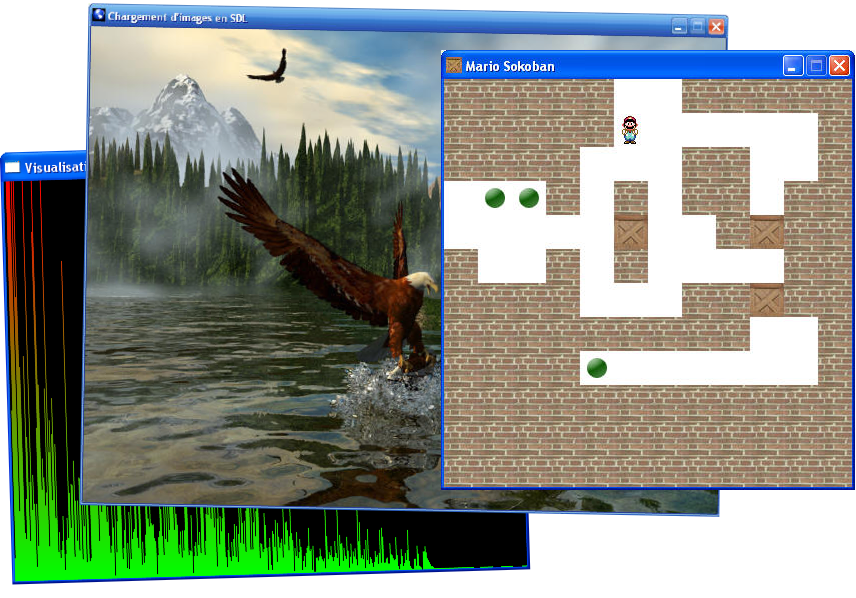
\includegraphics[height=0.4\textheight]{Introduction_original}\\
\small بعض الإنجازات الّتي سنقوم بها في هذا الكتاب
\end{figure}

\vfill
\hfill\parbox{0.3\textwidth}{\centering \textenglish{Mathieu Nebra}\\[0.2em]
مؤسس مشارك لموقع
\href{http://openclassrooms.com/}{\textenglish{OpenClassrooms}}
}

  \part{أساسيّات البرمجة بلغة الـ\textenglish{C}}
  \chapter{قلت برمجة ؟}
\section{ما هي البرمجة؟}
\begin{question}
  ما الذي تعنيه كلمة "بَرْمَجَ"؟
\end{question}

لن أتعبك وأعطيك أصل كلمة "بَرْمَجَ"، لكنني سأختصر كل شيء في جملة: البرمجة تعني إنشاء برامج حاسوب. وهذه البرامج التي تنشئها تأمر الجهاز بالقيام بتعليمات وأفعال معيّنة.
حاسوبك الخاص يحتوي على كثير من هذه البرامج وبمختلف أنواعها:

\begin{itemize}
  \item الآلة الحاسبة تعتبر برنامجاً.
  \item معالج النصوص يعتبر برنامجاً أيضاً.
  \item وكذلك برنامج المحادثة.
  \item ألعاب الفيديو هي برامج كذلك.
\end{itemize}

\Picture[\caption{نسخة عن لعبة \textenglish{MetalSlug} الشهيرة تم إنشاؤها من طرف العضو \href{http://www.siteduzero.com/membres-294-176405.html}{\textenglish{joe87}}}]{Chapter_I-1_MetalSlug}
باختصار البرامج موجودة في كل جهاز، وهي التي تعطي الحاسوب قدرته على إنجاز مختلف المهام التي تُخوَّل إليه. يمكنك أن تنشئ برنامج تشفير أو لعبة ثنائية / ثلاثية الأبعاد باستخدام لغة برمجة مثل \textenglish{C}.

ملاحظة: لم أقل أن إنشاء لعبة يتم برمشة عين، لقد قلت فقط بأنه شيء ممكن، لكن كن متأكداً، سوف يتطلب ذلك جهدا كبيراً!

وبما أننا في بداية الطريق، فإّننا لن نقوم بإنشاء لعبة ثلاثية الأبعاد! لكنّنا سنبدأ بكيفية عرض نص على الشاشة، طبعا ستقول ما علاقة هذا بإنشاء الألعاب؟ لكن ثِق بي، هذا الأمر ليس بسيطا كما يبدو!

بالطبع هذا ليس شيئا مُبهراَ، ولكن يجب علينا أن نبدأ من هنا؛ وشيئا فشيئا يمكنك أن تنشئ برامج معقّدة أكثر. فالهدف من هذا الدرس هو أن أعرفك على كل ما يتعلق بهذه اللغة.

\section{البرمجة، بأي لغة يا ترى؟}
حاسوبك هو آلة غريبة جداً، هذا أقل ما يمكن أن نقوله عنه. يمكننا أن نخاطبه فقط بالصفر والواحد، فمثلا إذا طلبنا منه حساب 3+5 فيمكن لهذا أن يعطينا نتيجة كالتالي (هذه ليست ترجمة دقيقة ولكنها تشبه ما يحدث بالفعل):\\
\InlineCode{0010110110010011010011110}

ما تَرَاه هنا يسمى اللغة الثنائية
(\textenglish{Binary language})
أو لغة الآلة
(\textenglish{Machine language})،
وحاسوبك لا يفهم سوى هذه اللغة، وكما تلاحظ، هذه اللغة غير مفهومة على الإطلاق!

مشكلتنا الآن:
\begin{question}
  كيف يمكننا التعامل مع حاسوب لا يفهم سوى اللغة الثنائية؟
\end{question}

حاسوبك لا يتحدث الإنجليزية، ولا العربية، ولا أي لغة غير هذه اللغة، ولكنها صعبة جدا لدرجة أن حتى أكبر خبراء الحاسوب لا يستخدمونها.
لهذا قام بعض مهندسي الحواسيب باختراع لغات يمكن أن تُتَرجَمَ إلى اللغة الثنائية، لكن الشيء الأصعب هو إنشاء البرامج الّتي تقوم بهذه الترجمة. ولحسن الحظ فقد قاموا بهذا العمل نيابة عنا. هذه البرامج تقوم بترجمة الأوامر الّتي تكتبها (مثلا: "أُحسب 3+5") إلى شيء يشبه هذا:
\InlineCode{0010110110010011010011110}.

هذا المخطط يلخص ما كنت أشرح:

\Picture{Chapter_I-1_Translation}

\section{قليل من المفردات}
حتّى الآن كنت أتحدّث إليك بكلمات بسيطة، لكن يجب أن تعلم أنه في المعلوماتية توجد مصطلحات علمية لكل ما ذكرت. طوال هذا الدرس، سوف تتعلم استخدام المفردات المناسبة. هذا سيفيدك كثيرا خصوصا عندما تتحدث مع مبرمجين آخرين، حيث أنك سوف تتفاهم معهم بكل سهولة.

نعود إلى الحديث عن المخطط السابق في المستطيل الأول قلت أن "برنامجك مكتوب بلغة مُبَسَّطة"، في الواقع هذا النوع من اللغات يُعرف باسم لغات البرمجة عالية المستوى (\textenglish{High-level programming languages}). هناك مستويات عديدة من لغات البرمجة، وكلما كان مستوى اللغة أعلى كانت أقرب إلى اللغة الحقيقية وكان استخدامها أسهل. إذن، اللغات عالية المستوى سهلة الاستخدام لكنها تتضمن بعض السلبيّات سوف نتعرّف عليها لاحقا.

توجد العديد من لغات البرمجة، وهي متفاوتة المستوى، منها:
\begin{itemize}
  \item \textenglish{C}
  \item \textenglish{C++}
  \item \textenglish{Java}
  \item \textenglish{Visual Basic}
  \item \textenglish{Delphi}
  \item و العديد غيرها
\end{itemize}

كما تلاحظ، لم أرتبها حسب مستوياتها، لذلك لا تعتقد أن اللغة الأولى في القائمة هي الأسهل أو العكس. عموما، لائحة اللغات الموجودة طويلة جدا لدرجة أنه لا يمكنني كتابتها كلها هنا.

مصطلح آخر يجب تذكّره هو
\underline{الشفرة المصدرية}
(\textenglish{Source code})،
 وهي ببساطة الشفرة الخاصة ببرنامجك الذي تكتبه بلغة عالية المستوى والذي يتم ترجمته فيما بعد إلى اللغة الثنائية.

 ثم يأتي دور البرنامج الذي يحوّل هذه اللغة عالية المستوى إلى اللغة الثنائية، هذا النوع من البرامج يعرف باسم
 \underline{المترجم}
  أو
  \underline{المصنّف}،
 والعملية الّتي يقوم بها تسمى
 \underline{الترجمة}
 أو
 \underline{التصنيف}.

\begin{information}
  يوجد لكل لغة عالية المستوى مترجم خاص، وهذا شيء منطقي، فاللغات مختلفة فيما بينها، فلا يمكننا ترجمة لغة
\textenglish{C}
بنفس الطريقة الّتي نترجم بها
\textenglish{Delphi}
مثلا.
  بعض اللغات مثل
\textenglish{C}
تملك العديد من المترجمات، فمنها من هو مكتوب من طرف
\textenglish{Microsoft}
، و منها من
\textenglish{GNU}
، إلخ… سوف نتعرّف على كل هذا في الدرس القادم.
  لحسن الحظ، هذه المترجمات متطابقة تقريبا (رغم وجود اختلافات طفيفة بينها سوف نتعرف عليها لاحقا).
\end{information}

أخيرا، البرنامج الثنائي المنشئ بواسطة المترجم يسمى الملف
\underline{القابل للتنفيذ}
أو
\underline{التنفيذي}
(\textenglish{Executable}).
 لهذا السبب تملك البرامج
 (على الأقل برامج
 \textenglish{Windows})
 الامتداد
\textenglish{.exe}
 والذي هو اختصار كلمة
 \textenglish{EXEcutable}.

 نعود إلى مخططنا السابق، وهذه المرة سنستخدم المصطلحات الصحيحة:

 \Picture{Chapter_I-1_Compilation}

 \section{لماذا نختار تعلّم \textenglish{C}؟}
 كما قلت سابقا، يوجد كثير من اللغات عالية المستوى، فلماذا ينبغي علينا أن نبدأ بإحداها على وجه الخصوص؟ سؤال عظيم!

على أية حال يجب علينا أن نختار بأي لغة سنبدأ البرمجة عاجلا أم آجلا، وبالتالي لديك الخيار في البدء بـ:
\begin{itemize}
  \item \textbf{لغة ذات مستوى عالي جدّا}:
 وتكون سهلة جدّا أوعامة، نذكر من بينها
 \textenglish{Python}، \textenglish{Ruby}، \textenglish{Visual Basic}،
 وغيرها. هذه اللغات تسمح بكتابة برامج بشكل أسرع. عامّة تحتاج لأن تُرفق معها ملفات مُسَاعِدة لكي تعمل (كَمُفَسِّرٍ مثلا).
  \item \textbf{لغة ذات مستوى منخفض قليلا}:
هي أكثر صعوبة نوعا ما، ولكن مع لغة مثل
\textenglish{C}
 سوف تتعلم كثيرا عن البرمجة وحول طريقة عمل حاسوبك. ستكون بعد ذلك قادراً على تعلّم لغة برمجة أخرى إن أردت وبكل يُسْرٍ.
\end{itemize}

من ناحية أخرى،
\textenglish{C}
لغة برمجة واسعة الإنتشار، أُستخدمت في برمجة العديد من البرامج التي تعرفها. حتى أنها كثيرا ما تدرّس في الدراسات العليا في مجال المعلوماتية.
هذه هي الأسباب الّتي جعلتني أتحمّس لتعليمك لغة
\textenglish{C}
بالتحديد. لم أقل أنّه يجب عليك أن تبدأ بها، لكنّي قلت إنه خيار جيّد لكي أقدّم لك معرفة صلبة في هذا الدرس.

\begin{information}
  بعض لغات البرمجة موجّهة أكثر للشبكة العنكبوتية
 (\textenglish{Web})
 مثل
 \textenglish{PHP}
 أكثر منها من إنشاء البرامج المعلوماتية.
\end{information}

سوف أفترض في هذا الكتاب أنّ هذه هي لغة برمجتك الأولى وأنّه لم يسبق لكم أن برمجت من قبل. فإن كنت قد برمجت قليلا من قبل فلا مضرّة في أن تعيد من الصفر.

\begin{question}
  ما هو الفرق بين
  \textenglish{C}
  و
  \textenglish{C++}
  ؟
\end{question}

هاتان اللغتان قريبتان جدّا من بعضهما، وكلاهما مستخدمتان بكثرة. ولكي تعرف كيف نشأتا يجب عليك أن تدرس التاريخ قليلا:
\begin{itemize}
  \item في البداية، عندما كانت الحواسيب تَزِنُ أطنانا وتشغل مكانا قَدْرُهُ حجم منزلك، تمّ إختراع لغة برمجة تسمّى
\textenglish{Algol}.
  \item بعدها تطوّرت الأمور أكثر واختُرعَت لغة برمجة جديدة عُرِفَتْ باسْمِ
\textenglish{CPL}
 والّتي تطوّرت فيما بعد إلى لغة
\textenglish{BCPL}
 ثم أخذت إسم اللغة
\textenglish{B}.
  \item مع مضيّ الزمن توصّل الخبراء إلى ابتكار اللغة
\textenglish{C}
 وقد تمّ إدخال بعض التعديلات عليها إلّا أنها لا تزال من أحد اللغات الأكثر استخداما اليوم.
  \item وبعد زمن، أراد الخبراء أن يضيفوا بعض الأشياء إلى
\textenglish{C}
، يمكن اعتبارها نوعا من التحسينات. والنتيجة كانت بما يعرف بلغة
\textenglish{C++}
، وهي لغة
\textenglish{C}
 مع إضافات تمكّننا من البرمجة بطريقة مختلفة.
\end{itemize}

\begin{information}
  الـ
\textenglish{C++}
ليست أحسن من الـ
\textenglish{C}
، هي فقط تمكننا من البرمجة بطريقة مختلفة وتساعد المبرمج على تنظيم شفرة برنامجه. رغم ذلك هي تشبه الـ
\textenglish{C}
كثيرا. وإن كنت تنوي تعلّم الـ
\textenglish{C++}
فيما بعد فَسَوْفَ تجد ذلك سهلا.
\end{information}

ولو اعتُبرت
\textenglish{C++}
 تطويرا لـ
\textenglish{C}
 فإن هذا لا يعني أنه يجب استخدام
\textenglish{C++}
 فقط لإنشاء البرامج. لغة
\textenglish{C}
 ليست لغة عجوزا منسيّة، بالعكس هي مستخدمة بكثرة اليوم. بل إنها أساس أنظمة التشغيل الكبيرة مثل
\textenglish{Unix }
(ومنه
\textenglish{GNU/Linux}
 و
\textenglish{Mac OS}) و
\textenglish{Windows}.

\section{هل البرمجة صعبة؟}
هذا سؤال يعذّب روح كل من يريد تعلّم البرمجة! هل يجب أن تكون أستاذ رياضيات كبير درس 10 سنوات من التعليم العالي حتّى تبدأ البرمجة؟

الجواب هو لا بالطبع. كل ما تحتاج إليه هو معرفة العمليات الأربع الأساسية:
\begin{itemize}
  \item الجمع
  \item الطرح
  \item الضرب
  \item القسمة
\end{itemize}
هذا ليس مخيفا! سوف أشرح لك في درس لاحق كيف يقوم الحاسوب بهذه العمليات الأساسية في برامجك.

باختصار، لا توجد صعوبات غير قابلة للحلّ. في الواقع، هذا يعتمد على طبيعة برنامجك، فإذا كنت تريد إنشاء برنامج تشفير فيجب عليك معرفة بعض الأشياء في الرياضيات، وإن كان برنامجك يقوم بالرسم ثلاثي الأبعاد فيجب أن تكون لديك بعض المعرفة بالهندسة الفضائية.

كل حالة تعامل بطريقة خاصّة. ولكن لتعلّم لغة
\textenglish{C}
 نفسها لا تحتاج إلى أيّة معارف قبليّة.

\begin{question}
  إذن أين هو الفخ؟ وأين تكمن الصعوبة؟
\end{question}

يجب أن تعرف كيف يعمل الحاسوب، لتفهم ما الّذي نقوم به في C. من هذا المنطلق، كن متيقّنا أنّي سأعلّمك كلّ هذا شيئا فشيئا.

اعلم أن للمبرمج صفات أيضا مثل:
\begin{itemize}
  \item الصبر: البرنامج لا يعمل عادة من أوّل محاولة، يجب أن تكون مثابراً.
  \item حسّ المنطق: صحيح أنّك لست بحاجة إلى أن يكون لديك مستوى جيّد في الرياضيّات، لكنّ هذا لا يمنع من التفكير وتحليل المشكلات بالمنطق.
  \item الهدوء: فيجب عليك ألّا تضرب حاسوبك بالمطرقة، فهذا لن يجعل برنامجك يعمل!
\end{itemize}

  \chapter{الحصول على الأدوات اللازمة}

بعد تجاوزنا لفصل تمهيدي مليئ بالثرثرة سوف نبدأ بالدخول في صلب الموضوع. سوف نجيب عن السؤال التالي : "ما هي البرامج التي نحتاج إليها للبدء في البرمجة ؟".

لا يوجد شيء صعب في هذا الفصل، سوف نأخذ وقتنا للتأقلم على هذه البرامج الجديدة.

اغتنم الفرصة ! في الفصل التالي سنبدأ حقّا في البرمجة و لن يكون هناك وقت للقيلولة !

\section{الأدوات اللازمة للمبرمج}

إذن ما هي الأدوات التي نحتاج إليها ؟
إذا تابعت الفصل السابق جيّدا، فستعرف واحدا على الأقل !

هل تعلم عمّا أتحدّث ؟ حقّا لا ؟

حسنا، نحن نتحدّث عن
\textbf{المترجم}
الذي يمكّن من ترجمة لغة الـ\textenglish{C}
إلى اللغة الثنائيّة !

كما قلت لك في الفصل الأوّل، يوجد العديد من المترجمات للغة الـ\textenglish{C}.
سنرى أن اختيار المترجم ليس أمرا معقّدا في حالتنا هذه.

ما الذي نحتاج إليه أيضا ؟ لن أتركك تخمّن كثيرا و سأعطيك القائمة :

\begin{itemize}
  \item \textbf{محرّر نصوص }
(\textenglish{Text Editor})
لكتابة الشفرة المصدرية الخاصّة بالبرنامح. نظريّا برنامج تحرير نصوص بسيط مثل
\textenglish{Notepad}
على
\textenglish{Windows}
أو
\textenglish{vi}
على
\textenglish{Unix}
يكفي، لكن من الأحسن استخدام محرّر نصوص ذكيّ يقوم بتلوين الشفرة المصدرية لكي يسهّل عليك العمل.
  \item \textbf{مترجم}
  لتحويل الشفرة المصدرية إلى ملف ثنائي.
  \item \textbf{المنقّح}
(\textenglish{Debugger})
لمساعدك على كشف الأخطاء في برنامجك. لسوء الحظ، لم نتمكّن بعد من ابتكار "المصحّح" الّذي يصحّح أخطائك لوحده. لكن، إن أحسنت استخدام المنقّح، يمكنك ببساطة إيجاد الأخطاء.
\end{itemize}

وجود مكتشف الأخطاء لا يعنى أن تتصرف بتهوّر و تسرع في كتابة برنامج مليء بالأخطاء، بل تريّث و كن هادئاً.

من الآن لدينا خياران :

\begin{itemize}
  \item إمّا أن نحصل على البرامج الثلاثة متفرّقة و هذه هي الطريقة الأكثر تعقيدا، و لكنّها تعمل. على
\textenglish{GNU/Linux}
تحديدا، عدد كبير من المبرمجين يفضّلون استخدام كلّ برنامج على حدة. لن أشرح هذه الطريقة هنا، بل سأتحدّث عن الطريقة الأسهل.
  \item أو أن تحصل على برنامج "ثلاثة في واحد" يتضمّن محرّر النصوص و المترجم و المنقّح. هذا النوع من البرامج يعرف باسم "بيئات التطوير المتكاملة"
(\textenglish{Integrated Development Environments})
و تسمّى اختصارا
\textenglish{IDE}.
\end{itemize}

يوجد العديد من بيئات التطوير. بداية، قد تواجه صعوبة في اختيار البيئة الملائمة لك. الشيء الأكيد هو : أي بيئة مهما كانت ستحقق لك العمل المطلوب.

\subsection{اختيار البيئة الخاصة بك}

بدا لي أنه من الأفضل أن أريك بعضا من البيئات الشهيرة و المجانيّة في نفس الوقت. شخصيّا، أنا أستخدمها جميعا و أختار في كل يوم  واحدا منها.

\begin{itemize}
  \item أحد هذه البيئات الّتي أفضّلها هو
\textbf{\textenglish{Code::Blocks}}.
هو مجّاني و يعمل على أغلب أنظمة التشغيل. أنصح كلّ مبتدئ أن يختاره للبدء (و في ما بعد أيضا إذا شعرت أنّه يلائمك جيّدا !).

يعمل على أنظمة التشغيل
\textenglish{Windows}،
\textenglish{Mac OS}
و
\textenglish{GNU/Linux}.
  \item الأكثر شهرة على
\textenglish{Windows}
هو الّذي أنشأته
\textenglish{Microsoft}،
إنّه
\textbf{\textenglish{Visual C++}}.
هو برنامج مدفوع (و باهظ الثمن) لكن لحسن الحظّ توجد نسخة مجانية منه تسمّى
\textbf{\textenglish{Visual Studio Express}}
(أنا أستخدم النسخة القديمة
\textbf{\textenglish{Visual C++ Express}}
في هذا الكتاب). و هي ممتازة جدّا (بينها و بين النسخة المدفوعة فوارق طفيفة). إنه برنامج كامل و يملك منقّحا قويّا.

يعمل على
\textenglish{Windows}
فقط.
  \item على
\textenglish{Mac OS X}
يمكنك استخدام
\textbf{\textenglish{Xcode}}
الّذي يفترض أن يكون متوفّرا على قرص تثبيت النظام. يناسب كثيرا مبرمجي
\textenglish{Mac}.

يعمل على
\textenglish{Mac OS X}
فقط.
\end{itemize}

\begin{information}
  ملاحظة لمستخدمي
  \textenglish{GNU/Linux} :
  يوجد العديد من البيئات لهذا النظام، و لكن المبرمجين المحترفين قد يفضّلون تجاوز البيئات و القيام بالترجمة "يدويّا"، و هو شيء أصعب قليلا. نحن سنبدأ باستخدام بيئات تطويرية. لذلك أنصحك بثبيت
  \textenglish{Code::Blocks}
  إن كنت على
  \textenglish{GNU/Linux}
  لكي تتمكن من متابعة شروحاتي.
\end{information}

\begin{question}
من هي البيئة الأفضل من بين كلّ بيئات التطوير هذه؟
\end{question}

كل واحدة من هذه البيئات تمكنك من البرمجة و متابعة بقيّة الكتاب من دون أيّة مشاكل. بعضها كامل أكثر من ناحية المميزات، و أخرى سهلة الإستخدام أكثر، ولكن في كلّ الأحوال البرامج الّتي تنشؤها تكون ذاتها أيّا كانت البيئة التي اِخْتَرْتها. فهذا الخيار ليس بالأهمّية الّتي تعتقدها.

في هذا الكتاب سوف أستخدم
\textenglish{Code::Blocks}.
فإن أردت الحصول على نفس لقطات الشاشة خاصّتي، خصوصا لكي لا تضيع في البداية، أنصحك بِدَايَةً بتثبيت
\textenglish{Code::Blocks}.

\section{\textenglish{Code::Blocks} (\textenglish{Windows, Mac OS X, GNU/Linux})}

\textenglish{Code::Blocks}
هي بيئة تطوير متكاملة حرّة و مجانيّة، متوفّرة للـ\textenglish{Windows}،
\textenglish{Mac}
و
\textenglish{GNU/Linux}.

حاليّا
\textenglish{Code::Blocks}
متوفّر بالإنجليزيّة فقط. لكن هذا ليس أمرا يدعوك إلى تجنّب استخدامه ! فنحن قلّما نحتاج إلى العمل بقوائم واجهته، فلغة
\textenglish{C}
هي الّتي تهمّنا.

كن على علم أنه عندما تبرمج سوف تقابل عادة توثيقا بالإنجليزية. هذا سبب آخر يدفعك للتدرّب على استخدام هذه اللغة.

\subsection{تنزيل \textenglish{Code::Blocks}}

توجّه إلى صفحة تنزيل
\textenglish{Code::Blocks}

\url{http://www.codeblocks.org/downloads/binaries}

ثمّ نزّل الملف الذي يناسب نظامك :

\begin{itemize}
  \item إذا كنت تستخدم
\textenglish{Windows}،
اذهب إلى القسم
"\textenglish{Windows}"
في أسفل الصفحة. نزّل البرنامج الّذي يحوي
\InlineCode{mingw}
في اسمه (مثلا :
\InlineCode{codeblocks-10.05mingw-setup.exe}).
النسخة الأخرى لا تحوي مترجما، لن تتمكن في حال استخدمتها من ترجمة برامجك !
  \item إذا كنت تستخدم
\textenglish{GNU/Linux}،
اختر الحزمة الّتي تناسب توزيعتك.

  \item إذا كنت تستخدم
\textenglish{Mac}،
اختر الملف الأحدث في القائمة، مثلا :
\InlineCode{codeblocks-10.05-p2-mac.zip}.

\end{itemize}

\begin{critical}
أقول و أكرّر : إذا كنت تستخدم
\textenglish{Windows}
فيجب عليك تنزيل النسخة الّتي يتضمَن اسمها كلمة
\textenglish{mingw}
لأنّه إذا اخترت النسخة الخاطئة فلن تتمكّن من ترجمة برامجك فيما بعد !
\end{critical}

التثبيت بسيط و سريع.  أترك جميع الخيارات كما هي و شغّل البرنامج. سوف تظهر لك نافذة شبيهة بهذه :

\begin{figure}[H]
	\centering
	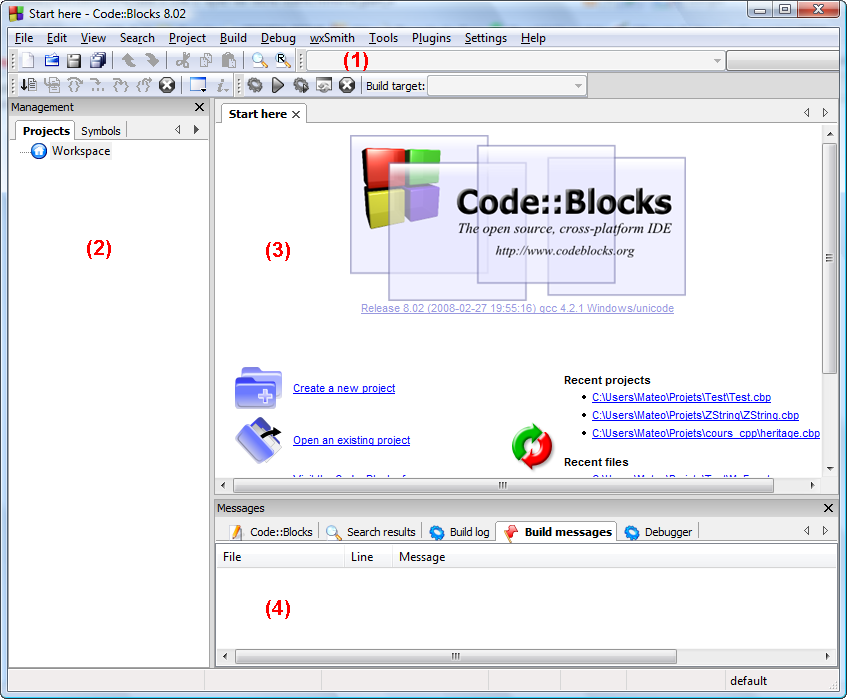
\includegraphics[width=\textwidth]{Chapter_I-2_CodeBlocks}
\end{figure}

نميّز أربعة أقسام رئيسية في واجهة البرنامج، و هي مرقّمة في الصورة :

\begin{enumerate}
  \item شريط الأدوات
(\textenglish{Toolbar}) :
يحتوي على كثير من الأزرار و لكنّنا سوف نستخدم بعضها فقط باستمرار، سأعود للحديث عن هذا فيما بعد.
  \item قائمة ملفات المشروع : توجد بيسار النافذة، تحتوي على كلّ الملفات المصدريّة المتعلقة بالبرنامج الذي تعمل عليه. تكون فارغة في البداية لأننا لم ننشئ أي ملف لحد الآن. سوف نبدأ بملأها خلال خمس دقائق من الآن بتقدّمك في هذا الفصل.
  \item المنطقة الرئيسية : هنا المساحة التي تكتب فيها الشفرة المصدرية الخاصة ببرنامجك بلغة الـ\textenglish{C}.
  \item منطقة الإشعار : و يدعوها البعض "منطقة الموت"، هنا تُعْرَضُ أخطاء الترجمة إذا كانت شفرة البرنامج تحوي خطأً ما. هذا الشيء يحدث كثيرا !
\end{enumerate}

ما يهمّنا الآن هو قسم محدد من شريط الأدوات. تجد فيه الأزرار التالية (بهذا الترتيب) :
\InlineCode{Compile}،
\InlineCode{Execute}،
\InlineCode{Compile \& Execute}،
\InlineCode{Recompile everything}
تذكّرهم جيّدا لأننا سنستخدمهم بانتظام.

\begin{figure}[H]
	\centering
	
\includegraphics{Chapter_I-2_Compile-toolbar}
\end{figure}

و هذا شرح عمل كلّ واحد من هذه الأزرار :

\begin{itemize}
  \item \textbf{\textenglish{Compile}} :
كل ملفّات الشفرة المصدرية الّتي كتبتها يتم ارسالها إلى المترجم الّذي يقوم بإنشاء الملف التنفيذي في حالة عدم وجود أخطاء. أمّا في حالة العثور على أخطاء (و هذا سيحدث عاجلا أم آجلا~!) فلن يتمّ إنشاؤه بل يعرض رسائل خطأ في منطقة الإشعار.
  \item \textbf{\textenglish{Execute}} :
يقوم بتشغيل آخر ملف تنفيذي تمّت ترجمته. يعني أنك ستستخدم هذا الزر لاختبار برامجك الّتي أنشأتها. طبعا يجب عليك ترجمة البرنامج قبل تشغيله. يمكننا أيضا استخدام الزرّ الثالث.
  \item \textbf{\textenglish{Compile \& Execute}} :
لا يجب أن تكون عبقريا لكي تعرف أنّه ليس إلا مجموع الزرّين السابقين. في الواقع هذا هو الزرّ الّذي ستستخدمه أكثر. في حالة ما إذا حدثت أخطاء في الترجمة لن يتمّ تشغيل البرنامج بل ستُعرض قائمة جميلة من الأخطاء التي يجب عليك تصحيحها أوّلا !
  \item \textbf{\textenglish{Recompile everything}} :
 عندما نستخدم
\textbf{\textenglish{Compile}}
يقوم
\textenglish{Code::Blocks}
في الحقيقة بترجمة الملفات الّتي عدّلتها فقط. أحيانا -فقط أحيانا- قد تحتاج إلى إعادة ترجمة جميع الملفّات. سنتحدّث لاحقا عن فائدة هذا الزر و أيضا عن كيفية عمل الترجمة بمزيد من التفصيل. حاليا لكي لا تختلط الأمور عليك يمكنك أن تعتبر أنّه غير مهمّ.
\end{itemize}

\begin{information}
أنصحك باستخدام اختصارات لوحة المفاتيح بدلا من الضغط على الأزرار، لأنّه شيء نكرّره كثيرا. تذكّر خصوصا أنّه يمكنك الضغط على
\InlineCode{F9}
بدل الزر
\InlineCode{Compile \& Execute}.
\end{information}

\subsection{إنشاء مشروع جديد}

لإنشاء مشروع جديد إذهب إلى قائمة
\InlineCode{File}
ثمّ
\InlineCode{New}
ثمّ
\InlineCode{Project}.
من النافذة الّتي تظهر اختر
\InlineCode{Console application}.

\begin{figure}[H]
	\centering
	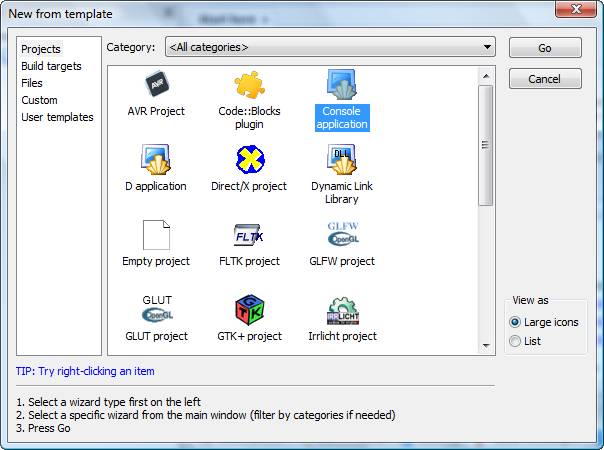
\includegraphics[width=0.8\textwidth]{Chapter_I-2_CodeBlocks-New-project}
\end{figure}

\begin{information}
كما تَرَى،
\textenglish{Code::Blocks}
يقترح عليك إنشاء عدد معتبر من أنواع البرامج الّتي تستخدم مكتبات
(\textenglish{Libraries})
معروفة مثل
\textenglish{SDL}
للـ\textenglish{2D}
و
\textenglish{OpenGL}
للـ\textenglish{3D}
و
\textenglish{Qt}
و
\textenglish{wxWidgets}
لإنشاء النوافذ الرسوميّة. حاليّا، هذه الأيقونات ليست سوى للزينة لأنّ المكتبات السابقة غير مثبّتة على حاسوبك لهذا لا يمكنك أن تجعلها تعمل. سوف نعود لهذه الأنواع الأخرى لاحقا. في هذه الأثناء لا يمكننا سوى أن نستخدم الـ\textenglish{Console}
لأنّك لا تملك بعد المستوى اللازم لانشاء أنواع أخرى من البرامج.
\end{information}

أنقر على
\InlineCode{Go}
لانشاء المشروع الجديد. ثم أنقر على
\InlineCode{Next}
فالصفحة الأولى ليس مهمّة. بعدها سيأتيك اختيار بين لغتي الـ\textenglish{C}
أو الـ\textenglish{C++}،
اختر الـ\textenglish{C}.

\begin{figure}[H]
	\centering
	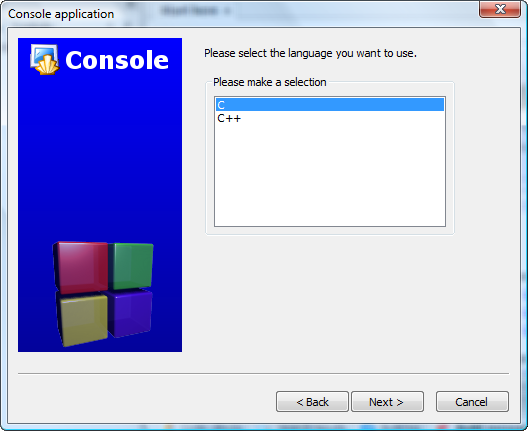
\includegraphics[width=0.8\textwidth]{Chapter_I-2_CodeBlocks-C}
\end{figure}

سيُطْلَبُ منك الآن إدخال اسم المشروع، و كذلك مسار المجلّد الذي تختاره لحفظ الملفّات فيه.

\begin{figure}[H]
	\centering
	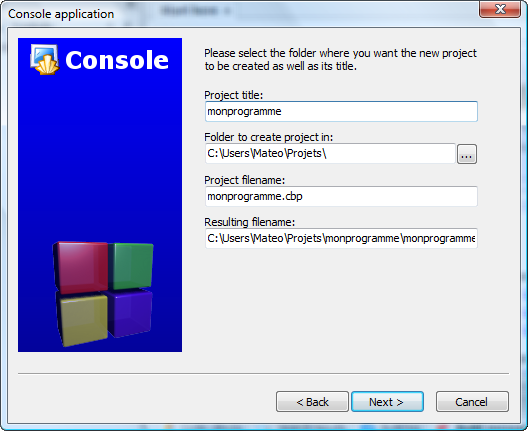
\includegraphics[width=0.8\textwidth]{Chapter_I-2_CodeBlocks_project-path}
\end{figure}

آخر خطوة تُطلب منك هي ، كيف ينبغي أن يترجم البرنامج، يمكنك ترك الخيارات على حالها، لن يكون لهذا أي تأثير على ما سنقوم به الآن (تأكّد أن إحدى الخانتين
"\textenglish{Release}"
أو
"\textenglish{Debug}"
تكون محدّدة على الأقل).

\begin{figure}[H]
	\centering
	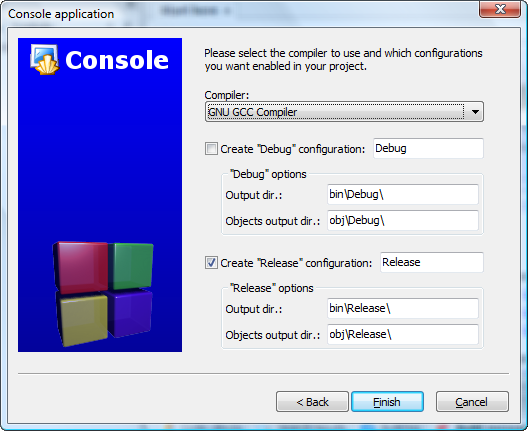
\includegraphics[width=0.8\textwidth]{Chapter_I-2_CodeBlocks_Compiler}
\end{figure}

إضغط على
\InlineCode{Finish}،
إنتهى !\\
لقد قام
\textenglish{Code::Blocks}
بإنشاء المشروع الأوّل و ملئه ببعض الشفرة المصدرية.

في الخانة الخاصة بالمشاريع على اليسار، قم بتوسيعها بالضغط على
'\InlineCode{+}'
لكي تظهر قائمة الملفات في المشروع. سيكون لديك على الأقل ملف يسمّى
\InlineCode{main.c}.
هذا هو كلّ شيء !

\section{\textenglish{Visual C++} (\textenglish{Windows} فقط)}

بعض التذكيرات حول
\textenglish{Visual C++} :

\begin{itemize}
  \item إنها البيئة التطويرية الخاصة بـ\textenglish{Microsoft}.
  \item برنامج مدفوع في الأصل، لكن توجد نسخة مجّانية منه تسمّى \textenglish{Visual C++ Express}.
  \item تمكّن من البرمجة باستخدام كلتا اللغتين
\textenglish{C}
و
\textenglish{C++}
(و ليس فقط
\textenglish{C++}
كما يوحي الاسم).
\end{itemize}

طبعا ستقوم بتحميل النسخة المجانية
\textenglish{Visual C++ Express}
(احذر، هو غير متوافق مع
\textenglish{Windows 7}
إلّا بداية من النسخة 2010) :

\begin{figure}[H]
	\centering
	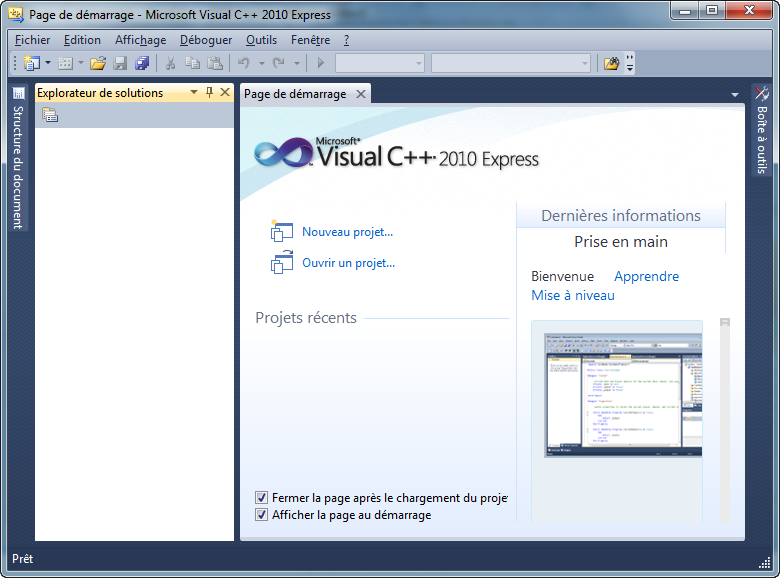
\includegraphics[width=\textwidth]{Chapter_I-2_Visual-Cpp}
\end{figure}

\begin{question}
ما الفرق بين هذه النسخة و النسخة "الحقيقيّة" ؟
\end{question}

لا تحتوي على محرّر موارد يسمح لك برسم الصور، الأيقونات أو النوافذ. هذا لا يهمّنا لأنّنا لن نحتاج إلى هذه الوظائف في هذا الكتاب. وجود هذه الوظائف أمر مستحسن لكنّه ليس لازما.

للتنزيل، زر موقع
\textenglish{Visual C++}.

\url{https://msdn.microsoft.com/fr-fr/express/aa975050.aspx}

و اختر تنزيل
\textenglish{Community 2015}
و اختر لغتك المفضّلة.

\subsection{التثبيت}

التثبيت سهل. سوف يقوم البرنامج بتحميل آخر نسخة من الأنترنت تلقائيا.\\
أنصحك بترك الخيارات كما هي.

بعد ذلك سيطلب منك التسجيل في غضون 30 يوما. لا تقلق، إنه سريع و مجاني لكن يجب القيام بذلك.

اضغط على الرابط المُعطى لك، ستدخل موقع
\textenglish{Microsoft}.
سجّل دخولك باستخدام
\textenglish{Windows Live ID}
(المكافئ لحساب
\textenglish{Hotmail}
أو
\textenglish{MSN})
أو قم بإنشاء واحد إذا لم يكن لديك، ثم أجب بعد ذلك على الأسئلة.

سيتم إعطاؤك في النهاية مفتاح تفعيل. انسخ هذا المفتاح في القائمة
\InlineCode{?}
ثم
"تسجيل المنتج".

\subsection{إنشاء مشروع جديد}

لإنشاء مشروع جديد، إذهب إلى قائمة
"ملف"
(\InlineCode{File})
ثمّ
"جديد"
(\InlineCode{New})
ثم
"مشروع"
(\InlineCode{Project}).
اختر
\InlineCode{Win32}
في العمود الأيسر ثمّ
\InlineCode{Win32 Console Application}.
ثمّ أدْخِل اسم مشروعك.

\begin{figure}[H]
	\centering
	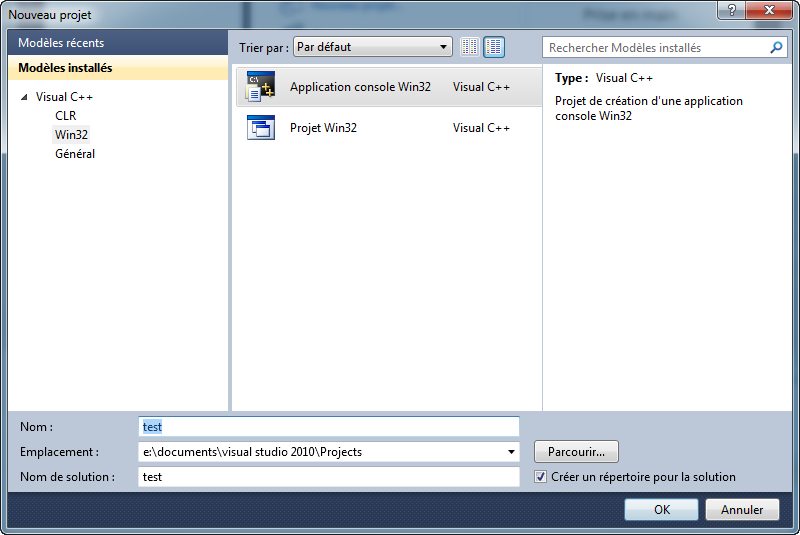
\includegraphics[width=0.8\textwidth]{Chapter_I-2_Visual-Cpp-New-project}
\end{figure}

وافق، ستظهر لك نافذة جديدة.

\begin{figure}[H]
	\centering
	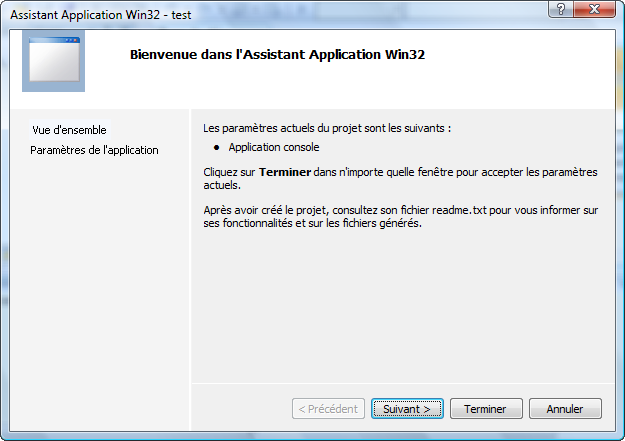
\includegraphics[width=0.8\textwidth]{Chapter_I-2_Visual-Cpp-Welcome}
\end{figure}

هذه النافذة لا تحوي أيّ شيء مهمّ، تابع فقط.

\begin{figure}[H]
	\centering
	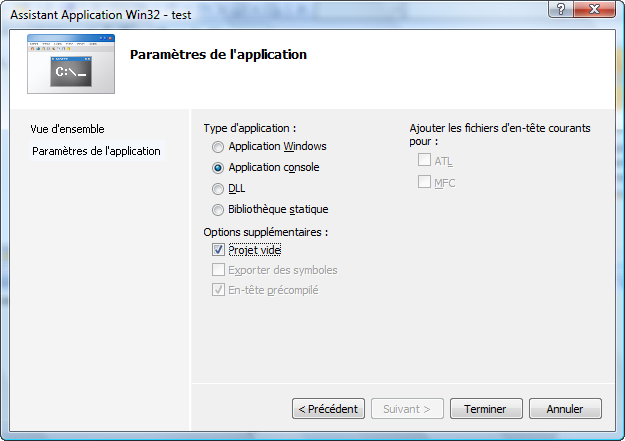
\includegraphics[width=0.8\textwidth]{Chapter_I-2_Visual-Cpp-Parameters}
\end{figure}

اختر
\InlineCode{Console application}
و تأكّد من إنشاء مشروع فارغ عن طريق تحديد
\InlineCode{Empty project}،
ثم اضغط على
"إنهاء"
(\InlineCode{Finish}).

\subsection{إضافة ملف مصدري جديد}

مشروعك فارغ لحدّ الآن. لإضافة ملف مصدري، اضغط باليمين على
"الملفات المصدرية"
(\InlineCode{Source files})
الموجود على اليسار، ثمّ اختر
"إضافة"
(\InlineCode{Add})
ثمّ
"عنصر جديد"
(\InlineCode{New element}).

\begin{figure}[H]
	\centering
	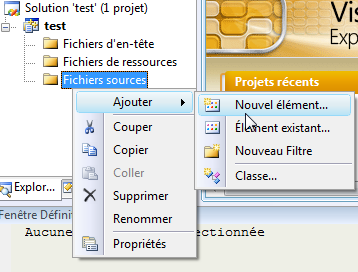
\includegraphics[width=0.5\textwidth]{Chapter_I-2_Visual-Cpp-New-source}
\end{figure}

اختر
\InlineCode{Visual C++}
على اليسار ثمّ
\InlineCode{C++ File}
(أعلمُ أنّنا لا ندرس
\textenglish{C++}
و لكن ليس لهذا أهميّة هنا). أدْخِل اسم الملف :
\InlineCode{main.c}

\begin{figure}[H]
	\centering
	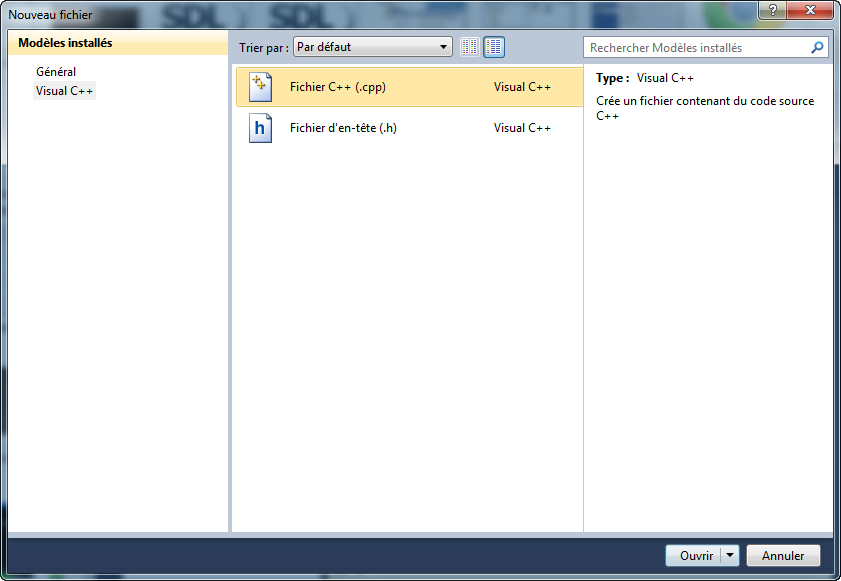
\includegraphics[width=0.8\textwidth]{Chapter_I-2_Visual-Cpp-New-file}
\end{figure}


ثم اضغط على
"إضافة"
(\InlineCode{Add}).
سيتم إنشاء ملفّ فارغ. أنصحك بحفظه بسرعة باسم
\InlineCode{main.c}.

انتهى، يمكنك الآن أن تبدأ في كتابة الشفرة.

\subsection{النافذة الرئيسيّة}

لنرى ما هي أهمّ أقسام النافذة الرئيسيّة في
\textenglish{Visual C++ Express}.

\begin{figure}[H]
	\centering
	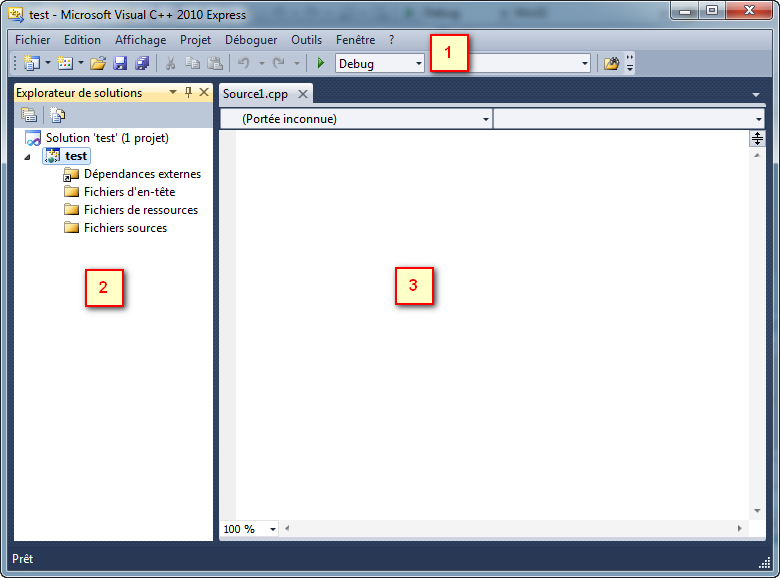
\includegraphics[width=\textwidth]{Chapter_I-2_Visual-Cpp-main}
\end{figure}

هذه النافذة تشبه مثيلتها في
\textenglish{Code::Blocks}.
و لكن رغم ذلك سوف نعيد رؤية معنى كلّ جزء.

\begin{enumerate}
  \item شريط الأدوات : فيه أزرار اعتيادية. لكن كما ترى لا يوجد أيّ زرّ للترجمة. يمكنك إضافته عن طريق النقر باليمين على هذا الشريط و اختيار
"تنقيح"
(\InlineCode{Debug})
و
"توليد"
(\InlineCode{Generate})
من القائمة.

كلّ هذه الأزرار لديها ما يكافئها في القوائم
\InlineCode{Debug}
و
\InlineCode{Generate}.
استخدام
\InlineCode{Generate}
ينشئ الملف التنفيذي (أي أنها تعني الترجمة). إذا استخدمت
\InlineCode{Debug / Execute}
فسوف يقترح عليك الترجمة قبل التشغيل. إختصارات لوحة المفاتيح :
\InlineCode{F7}
لتوليد المشروع و
\InlineCode{F5}
لتشغيله.
  \item هذه المساحة جدّ مهمّة، إذ أنها تحتوي على الملفات الخاصة بمشروعك. أنقر على
"مستكشف الحلول"
(\InlineCode{Solution explorer})
في الأسفل إن لم يكن فُعِل من قبل. سوف ترى أنّه قد تمّ إنشاء مجلّدات لفصل أنواع الملفّات المختلفة (مصدريّة، رأسيّة و موارد). سنتعرف لاحقا على مختلف أنواع الملفات التي تكوّن المشروع.
  \item المساحة الرئيسية : التي نعدّل فيها الملفّات المصدريّة.
\end{enumerate}

أكملنا جولتنا في
\textenglish{Visual C++}.
يمكنك إلقاء نظرة على
الخيارات
إن أردت لكن لا تأخذ من وقتك ثلاث ساعات هناك ! لأنه يوجد كثير منها.

\section{\textenglish{Xcode} (\textenglish{Mac OS X} فقط)}

هناك الكثير من البيئات التطويرية المتوافقة مع
\textenglish{Mac}
على غرار
\textenglish{Code::Blocks}
طبعا.\\
سأقدم لك البيئة الأكثر شهرة في الماك و هي
\textenglish{Xcode}.

\subsection{\textenglish{Xcode}،
 أين أنت ؟}

أغلب مستخدمي
\textenglish{Mac OS X}
ليسوا مبرمجين. لقد فهمت
\textenglish{Apple}
هذا، لذلك لم تثبّته افتراضيا مع النظام.\\
لحسن الحظ، لكلّ من يريد أن يبرمج، كلّ شيء جاهز.
\textenglish{Xcode}
متوفّر على
\textenglish{MacAppStore}.
ابدأ بأخذه من هناك.

أنصحك أيضا بإلقاء نظرة على الموقع الخاص بالمطوّرين لـ\textenglish{Apple}.

\url{https://developer.apple.com/}

سوف تجد هناك كمّا هائلا من من المعلومات المهمّة للتطوير على
\textenglish{Mac}.
يمكنك منه تحميل العديد من البرامج للتطوير.\\
لا تتردّد في التسجيل في
\textenglish{ADC} (\textenglish{Apple Development Connection})،
إنه مجاني و يساعدك على تتبع كل ما هو جديد.

\subsection{تشغيل \textenglish{Xcode}}

أوّل شيء يمكننا فعله هو إنشاء مشروع جديد، فلنبدأ بهذا. إذهب إلى
"ملف "
(\InlineCode{File})
ثمّ
"مشروع جديد"
(\InlineCode{New Project}).
ستفتح لك نافذة اختيار المشروع.

\begin{figure}[H]
	\centering
	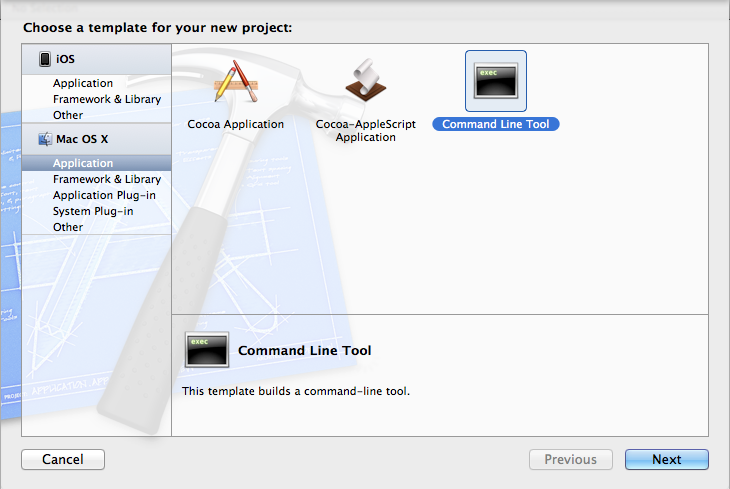
\includegraphics[width=0.8\textwidth]{Chapter_I-2_Xcode-New-project}
\end{figure}

اختر
\InlineCode{Application}
من اليسار ثمّ
\InlineCode{Command Line Tool}.
اضغط بعدها على
\InlineCode{Next}.
سوف يُطلب منكم بعدها حفظ مشروعك (كلّ مشروع يجب أن يحفظ منذ البداية) و اسمه. ضعه في المجلّد الّذي تريد.

بمجرّد إنشائه، سيتّم عرض مشروعك على شكل مجلّد يحتوي على العديد من الملفّات في الـ\InlineCode{Finder}.
الملف الّذي يملك الامتداد
\InlineCode{.xcodeproj}
يوافق ملف المشروع. إنه الملف الذي عليك اختياره في المرة القادمة لفتح مشروعك.

\subsection{نافذة التطوير}

في
\textenglish{Xcode}،
عندما تختار
\InlineCode{main.c}
تظهر لك نافذة شبيهة بهذه :

\begin{figure}[H]
	\centering
	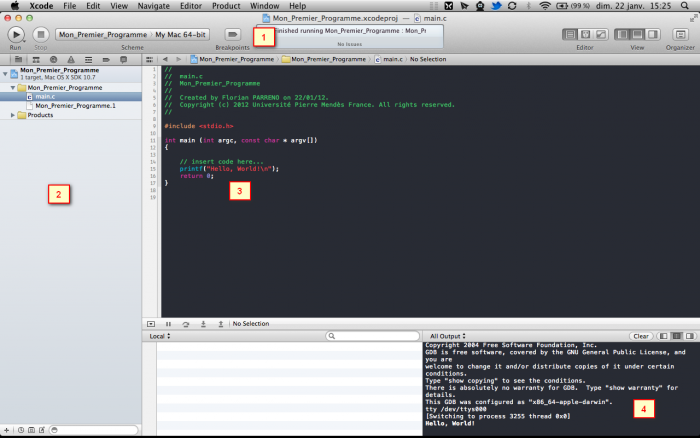
\includegraphics[width=\textwidth]{Chapter_I-2_Xcode-main}
\end{figure}

الواجهة مقسمة إلى أربعة أقسام، مرقمة هنا من 1 إلى 4 :

\begin{enumerate}
  \item الجزء الأوّل هو شريط الأزرار في الأعلى. أهمّ زرّ فيه هو
"تشغيل"
(\InlineCode{Run})
وظيفته تشغيل البرنامج.
  \item الجزء اليسار مخصص للتمثيل الشُجيري لمشروعك الخاص. بعض الأقسام تحتوي على الأخطاء، التحذيرات، إلخ. يقوم
\InlineCode{Xcode}
تلقائيّا بنقلك إلى القسم المهم. و هو الذي يحمل اسم المشروع.
  \item الجزء الثالث تتغيّر وظيفته حسب ما قمت بتحديده في الجزء الأيسر. و هنا يعرض محتوى الملف
\InlineCode{main.c}.
  \item أخيرا، الجزء الرابع يُظهر نتائج تشغيل البرنامج على الشاشة عندما تقوم بتشغيل البرنامج.
\end{enumerate}

\subsection{إضافة ملفّ جديد}

في البداية، لن تملك سوى ملف مصدري واحد و هو
\InlineCode{main.c}،
و لكن لاحقا عندما نتقدم في الدروس سأطلب منك إنشاء ملفات مصدريّة بنفسك، عندما تصبح برامجنا أكبر.

لإنشاء ملفّ جديد، اذهب إلى قائمة
\InlineCode{File}
ثمّ
\InlineCode{New File}.
سيطلب منك إدخال نوع الملف الذي تريد إنشاءه. توجّه إلى قائمة
\InlineCode{Mac OS X}
و اختر
\InlineCode{C and C++}
ثمّ
\InlineCode{C File}.
لاحظ هذه الصورة.

\begin{figure}[H]
	\centering
	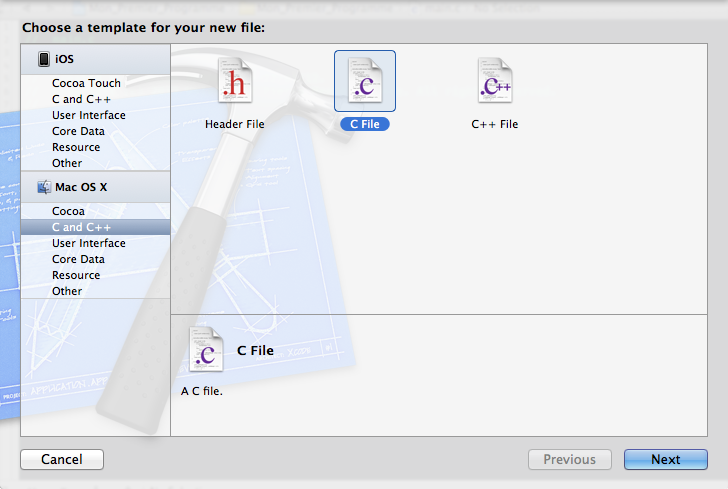
\includegraphics[width=0.8\textwidth]{Chapter_I-2_Xcode-C}
\end{figure}

يجب عليك إعطاء اسم لملفّك الجديد. امتداده يجب أن يبقى
\InlineCode{.c}.
أحيانا -كما سنرى لاحقا- يجب عليك أيضا إنشاء ملفّات بامتداد
\InlineCode{.h}.
الخانة
\InlineCode{Also create file.h}
مخصّصة لهذا الغرض. حاليّا هذا الخيار لا يهمّنا.

انقر بعدها على
\InlineCode{Finish}.
انتهى ! أصبح في مشروعك ملفٌ آخر غير الملف
\InlineCode{main.c}،
هنيئا لك فقد أصبحت الآن جاهزاً للبرمجة على الـ\InlineCode{Mac}.

\section*{ملخّص}

\begin{itemize}
  \item المبرمجون يحتاجون إلى ثلاثة أدوات : محرّر نصوص، مترجم و منقّح.
  \item من الممكن تثبيت هذه الأدوات منفصلة، لكنّه من المعتاد البوم الحصول على حُزمةٍ ثلاثة-في-واحد نسميها بيئة التطوير المتكاملة.
  \item \textenglish{Code::Blocks}،
\textenglish{Visual C++}،
و
\textenglish{Xcode}
تعدّ من بين بيئات التطوير الأكثر شهرة.
\end{itemize}

  \chapter{برنامجك الأوّل}

لقد قمنا بتحضير كلّ شيء إلى حد الآن ويمكننا أن نبدأ قليلا من البرمجة. مع نهاية هذا الفصل ستكون قد نجحت في إنشاء أوّل برنامج لك.

لكي أصدقك القول، سيظهر البرنامج بالأبيض والأسود ولن يقوم بشيء سوى إلقاء التحيّة. يبدو عديم الفائدة، لكنّه برنامجك الأوّل وأؤكّد لك أنّك ستكون فخورا به.

\section{كونسول أو نافذة ؟}

لقد تحدثنا سابقا عن فكرة برامج الكونسول وبرامج النوافذ في الفصل السابق. البيئة التطويرية تطلب منا تحديد أي نوع من البرامج نريد أن ننشئها. ولقد قلنا إننا سننشئ برامج من نوع كونسول.

يوجد نوعان من البرامج، لا أكثر :

\begin{itemize}
  \item ،برامج بنوافذ
  \item برامج تعمل في الكونسول.
\end{itemize}

\subsection{البرامج الّتي تملك نوافذ}

هي البرامج التي نعرفها جميعا. هذا مثال على برنامج من نوع نافذة، مثل الرسام.

\begin{figure}[H]
	\centering
	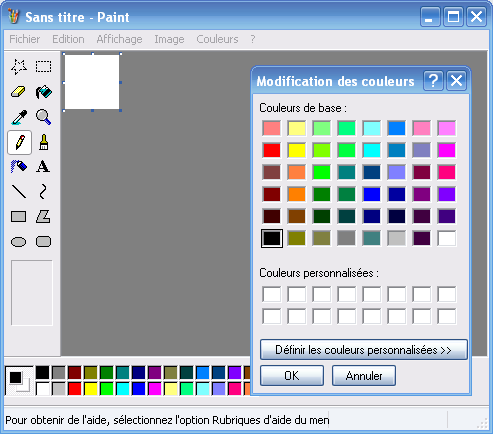
\includegraphics[width=0.6\textwidth]{Chapter_I-3_Paint}
\end{figure}

أعتقد أنّك تحب إنشاء برامج كهذه، لكنّ هذا ليس في مقدورك حاليا. في الواقع، إنشاء برامج بنوافذ هو أمر ممكن بلغة \textenglish{C}، لكنّ بالنسبة لمبتدئ، هذا أمر معقّد جدّا. كبداية، يستحسن إنشاء برامج الكونسول.

\begin{question}
  لكن ماذا يعنى برنامج
\textenglish{Console}
؟
\end{question}

\subsection{البرامج الّتي تعمل في الكونسول}

برامج الكونسول هي أول ما ظهر من برامج. في ذلك الوقت، شاشات الحواسيب لم تكن سوى بالأبيض والأسود، ولم تكن فعّالة لكي تتمكّن من رسم النوافذ كما هو الحال مع حواسيبنا حاليّا.

مرّ الزمن بسرعة وزادت شعبية الويندوز نظراً لبساطته إلى أن نسي كثير من الناس ما هي الكونسول.

لديّ خبر جيّد لك !
\textbf{الكونسول لم تمت بعد} !
 في الواقع،
\textenglish{GNU/Linux}
 قد أعاد الكونسول إلى الحياة. هذه صورة لكونسول على
\textenglish{GNU/Linux}.

\begin{figure}[H]
	\centering
	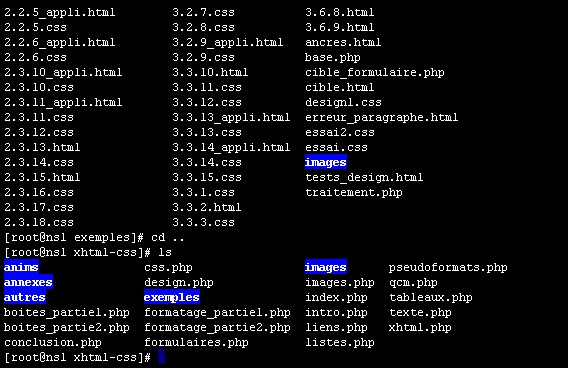
\includegraphics[width=0.6\textwidth]{Chapter_I-3_Console}
\end{figure}

مرعب ! صحيح ؟ لكن على الأقل عرفت ما هي الكونسول، وهذه بعض الملاحظات :

\begin{itemize}
  \item اليوم، يمكننا عرض الألوان في الكونسول. ليس كلّ شيء بالأبيض والأسود كما تتخيّل.
  \item الكونسول هو الأسهل من ناحية البرمجة بالنسبة للمبتدئين.
  \item أداة عالية الإمكانيّات إذا عرفنا كيف نستخدمه.
\end{itemize}

كما قلت لك، إنشاء برامج كونسول أمر سهل جدّا وملائم للمبتدئين (وهذا عكس برامج النوافذ). ليكن في علمك أيضا أنّ الكونسول قد تطوّرت وبإمكانها عرض الألوان، ولا شيء يمنعك من إضافة صورة خلفيّة لها.

\begin{question}
  وفي الويندوز ألا توجد
\textenglish{Console}
 ؟
\end{question}

بلى، لكنّها مخفيّة لو صح القول. يمكنك فتحها بالذهاب إلى "إبدأ"
(\InlineCode{Start})
 ثمّ "ملحقات"
(\InlineCode{Accessories})
 ثمّ "موجه الأوامر"
(\InlineCode{Command prompt})
 أو بالذهاب إلى "إبدأ" ثمّ "تشغيل"
(\InlineCode{Run})
 واكتب فيها
\InlineCode{cmd}
 واضغط على "موافق".

\begin{figure}[H]
	\centering
	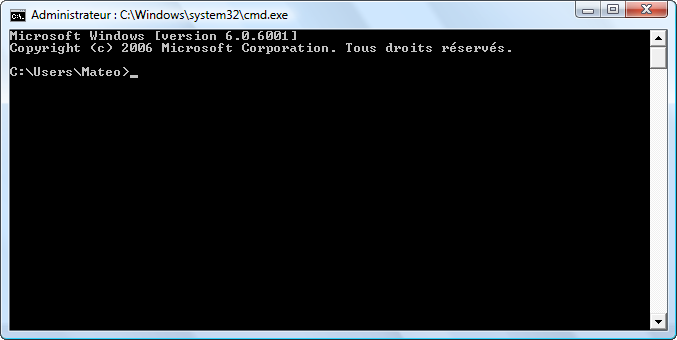
\includegraphics[width=0.6\textwidth]{Chapter_I-3_Console-Windows}
\end{figure}

إذا كنت تستخدم نظام ويندوز، فاعلم بأن أولى برامجك ستكون في نوافذ شبيهة بهذه. أنا لم أختر البداية هكذا لجعلك تشعر بالملل، بل لتعليمك الأساسيّات اللازمة لكي تتمكّن لاحقا من إنشاء النوافذ.

إذن فلتكن متيقّناً، بمجرّد أن تصل إلى المستوى اللازم لإنشاء النوافذ، سوف أعلّمك كيف تفعل ذلك.

\section{الحدّ الأدنى من الشفرة المصدرية}

من أجل أي برنامج، يجب كتابة قدر معيّن من الشفرة المصدرية. هذه الشفرة لا تقوم بشيء خاصّ لكنّها ضروريّة. هذه الشفرة التي سنكتشفها الآن ستكون أساس أغلب برامجك الّتي ستكتبها بلغة \textenglish{C}.

\subsection{أطلب من البيئة التطويرية الخاصة بك تزويدك بالحد الأدنى من الشفرة المصدرية}

لقد لاحظت أن طريقة إنشاء مشروع جديد تختلف من بيئة تطويرية إلى أخرى. إليك تذكيراً بسيطا : في برنامج
\textenglish{Code::Blocks}
 (الذي سنستخدمه في هذا الكتاب)، عليك التوجه نحو
\InlineCode{File}
 ثمّ
\InlineCode{New}
 ثمّ
\InlineCode{Project}
 ثم تختار
\InlineCode{Console Application}
 وبعدها اللغة
\textenglish{C}.
سيولّد لك الحد الأدنى من الشفرة المصدرية
 \textenglish{C}
 التي تحتاجها. ها هي :

\begin{Csource}
#include <stdio.h>
#include <stdlib.h>

int main()
{
    printf("Hello world!\n");
    return 0;
}

\end{Csource}

\begin{information}
لاحظ أنّه يوجد سطر فارغ في نهاية الشفرة. يفترض أن ينتهي كل ملف مكتوب بلغة
\textenglish{C}
هكذا. إن لم تفعل ذلك، فهذه ليست بمشكلة، لكن توقّع أن يعرض لك المترجم تحذيراً
(\textenglish{Warning}).
\end{information}

علماً أنّ السطر :
\begin{Csource}
int main()
\end{Csource}
\dots
بإمكانه أن يُكتب كالتالي :

\begin{Csource}
int main(int argc, char *argv[])
\end{Csource}

كلتا العبارتين تحملان نفس المعنى لكن الثانية، الأكثر تعقيدا، هي الأكثر شيوعا، لذلك فإنّنا سنستخدمها في الفصول القادمة.\\
إستخدامنا للشكل الأوّل أو الثاني لا يغيّر شيئا بالنسبة لنا. لذلك لا داعي لإضاعة الوقت هنا، خصوصاً أنّك لا تملك المستوى اللازم لفهم ما تعنيه.

إذا كنت تستخدم بيئة تطويرية أخرى فقم بنسخ هذه الشفرة المصدرية وألصقها في الملف \InlineCode{main.c} ليكون لديكم نفس الشفرة.

أخيرا، قم بحفظ عملك في المشروع. أعلم أننا لم نقم بشيء حتّى الآن لكن من الجيّد التعوّد على الحفظ في كلّ مرّة.

\subsection{تحليل أسطر الشفرة المصدرية السابقة}
قد تبدو لك الشفرة المصدرية السابقة أنّها كاللغة الصينيّة، أنا أتخيّل ذلك ! في الواقع هي تسمح بإنشاء برنامج كونسول يعرض نصّا على الشاشة. يجب تعلّم كيفيّة قراءة كلّ هذا.

فلنبدأ بأوّل سطرين :
\begin{Csource}
#include <stdio.h>
#include <stdlib.h>
\end{Csource}

هذان السطران يبدآن بعلامة
\InlineCode{\#}.
وهي أسطر خاصّة تُعرف باسم
\textbf{توجيهات المعالج القبلي}
(\textenglish{Preprocessor directives}). اسم معقّد، أليس كذلك ؟ هذه الأسطر تتمّ قراءتها من طرف البرنامج المسمّى بالمعالج القبلي، وهو برنامج يتمّ تشغيله في بداية الترجمة.

ما رأيناه سابقا كان مخطّطا بسيطا لعمليّة الترجمة. لكنّ في الواقع، هناك الكثير من المراحل التي تحدث في هذه العمليّة. سنقوم بتفصيل هذا لاحقا. حاليّا عليك فقط تذكّر وضع هذين السطرين أعلى كلّ ملفّاتك.

\begin{question}
  حسنا لكن ماذا يعنيه هذان السطران ؟ أريد أن أعرف !
\end{question}

كلمة
 \InlineCode{include}
 بالإنجليزيّة تعني "تضمين". هذان السطران يقومان بتضمين ملفّات في المشروع، أي إضافة هذه الملفّات من أجل عمليّة الترجمة. هناك سطران وبالتالي هناك ملفان يتمّ تضمينهما في المشروع وهما بالترتيب :
\InlineCode{stdio.h}
 و
\InlineCode{stdlib.h}.
هذان الملفّان موجودان بالفعل على حاسوبك وهما ملفّان مصدريّان جاهزان، سوف تعرف مستقبلا أنّنا نسميها
\textbf{مكتبات}
(\textenglish{Libraries}).
 هذه الملفّات تحتوي الشفرة المصدرية اللازمة لعرض نصّ على الشاشة.

 بدون هذين الملفّين، كتابة نصّ على الشاشة سيكون أمرا مستحيلاً. فالحاسوب لا يعرف فعل أي شيء مبدئيا.

 باختصار، السطران الأول والثاني يقومان بتضمين المكتبات التي ستساعدنا في إظهار نصّ على الشاشة بكلّ سهولة.

 نمر للتالي، باقي الأسطر :
 
\begin{Csource}
int main()
{
    printf("Hello world!\n");
    return 0;
}
\end{Csource}

ما تراه هنا هو ما نسميه بـ\textbf{التابع}
أو
\textbf{الدالّة}
(\textenglish{Function}).
 البرنامج في لغة
\textenglish{C}
 يتكوّن من مجموعة دوال. حاليّا برنامجنا لا يحوي سوى دالّة واحدة.

الدالّة تمكّننا من تجميع مجموعة من الأوامر. الغرض من تجميع الأوامر هو جعلها تقوم بوظيفة ما. مثلا يمكننا إنشاء دالّة باسم
 \InlineCode{open\_file}
 وجعلها تحتوي التعليمات التي تشرح للحاسوب كيفيّة فتح ملف.

 دون الدخول في تفاصيل إنشاء الدالّة (الوقت مبكّر، سوف نتحدّث عن الدوال في وقت لاحق) لنحلّل رغم ذلك أجزائه الكبيرة. السطر الأوّل يحتوي اسم الدالّة، إنّه الكلمة الثانية.\\
 أجل، اسم دالّتنا هو
\InlineCode{main}
والذي يعني
"الرئيسية"
. وتشغيل البرنامج دائما يبدأ من الدالة
\InlineCode{main}.

للدالّة بداية ونهاية، وهي محدودة بالحاضنتين
\InlineCode{\{}
و
\InlineCode{\}}.
محتوى الدالّة موجود بين هاتين الحاضنتين. إن كنت قد تابعت جيداً فقد عرفت أنّ الدالّة مشكّلة من سطرين :

\begin{Csource}
printf("Hello world!\n");
return 0;
\end{Csource}

هاته الأسطر في الداخل نسميها
\textbf{التعليمات}
(\textenglish{Instructions})
 (هذه إحدى المصطلحات الّتي يجب عليك حفظها). كلّ تعليمة تمثّل أمراً بالنسبة للحاسوب. فكلّ واحدة منها تطلب منه فعل شيء محدّد.

 كما قلت لك، بتجميع ذكيّ للتعليمات في الدالّة يمكننا إنشاء أجزاء برنامج جاهزة للاستخدام. باستخدام التعليمات المناسبة يمكننا إنشاء دالّة
 \InlineCode{open\_file}
 كما شرحت لك قبل قليل، و أيضا دالّة
\InlineCode{move\_character}
 في لعبة فيديو، على سبيل المثال.

 البرنامج في الواقع ما هو إلّا تتابع لتعليمات : إفعل هذا و إفعل ذاك. أنت تعطي أوامر للحاسوب و هو يقوم بتنفيذها.

 \begin{critical}
هامّ جدّا : لا بدّ أن تنتهي كلّ تعليمة بفاصلة منقوطة
"\InlineCode{;}"
. بهذا يمكن التفريق بين ما إذا كانت هذه تعليمة أم لا. إذا نسيت وضع فاصلة منقوطة نهاية تعليمة ما، فلن تتمّ ترجمة برنامجك.
 \end{critical}

 السطر الأول :
 \InlineCode{printf("Hello world!\\n");}
 يطلب إظهار الرسالة
 "\textenglish{Hello world!}"
  على الشاشة. عندما يصل برنامجك إلى هذا السطر، فسوف يقوم بعرض هذه الرسالة ثمّ المرور إلى التعليمة التالية.

  التعليمة التالية هي
\InlineCode{return 0;}
 و هي تخبرنا أنّ الدالّة
\InlineCode{main}
 قد انتهت و تطلب منه إعادة 0.

 \begin{question}
   لماذا يقوم برنامجي بإعادة العدد 0 ؟
 \end{question}

 في الواقع، كلّ برنامج عندما ينتهي يُرجع قيمة معينة. على سبيل المثال، ليقول أنّ كلّ شيء سار على ما يرام. عمليّا، 0 يعني  أنّ كلّ شيء سار على ما يرام، و كلّ قيمة أخرى تدلّ على حدوث خطأ. في أغلب الأحيان هذه القيمة لا تُستخدم ، لكن يجب رغم ذلك استعمالها.\\
 كان يمكن أن يعمل برنامجك بدون
 \InlineCode{return 0}
، لكن يمكننا القول أن وضعها يعتبر أمراً أكثر نظافة و أكثر جدّية.

إلى هنا نكون قد فصّلنا قليلا في عمل هذه الشفرة المصدرية.

طبعا، نحن لم ندرس كلّ شيء بعمق، و قد تكون لديك بعض الأسئلة عالقة في ذهنك. كن على يقين بأنك ستجد لها أجوبة شيئا فشيئا مع تقدّمنا في الكتاب. لا يمكنني أن أطلعك على كلّ شيء من البداية، لأنّ هناك كثيراً من الأشياء لاستيعابها.

إليك ما يلي : بما أنني في حال جيّدة، سأقوم بوضع مخطّط يضمّ المصطلحات الّتي تعلّمناها في هذا الفصل.

\begin{figure}[H]
	\centering
	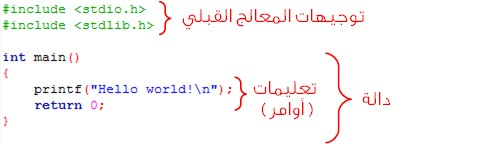
\includegraphics[width=0.8\textwidth]{Chapter_I-3_HelloWorld}
\end{figure}

\subsection{لنجرّب برنامجنا}

كلّ ما سنقوم به الآن هو ترجمة المشروع ثمّ تشغيله (اضغط على
\InlineCode{Build \& Run}
 إذا كنت على
\textenglish{Code::Blocks}).
سيطلب منك حفظ مشروعك إذا لم تقم بذلك من قبل.

\begin{critical}
  إن لم تنجح الترجمة و ظهر لك خطأ مثل :\\
\InlineCode{"My-program - Release" uses an invalid compiler. Skipping...}\\\InlineCode{Nothing to be done...}
فهذا يعني أنّك نزلت نسخة
\textenglish{Code::Blocks}
 دون
\InlineCode{mingw}
 (المترجم)، عد و نزّل النسخة التي تحتوي على
\InlineCode{mingw}.
\end{critical}

بعد بُرهة، يظهر برنامجك كما في الصورة :

\begin{figure}[H]
	\centering
	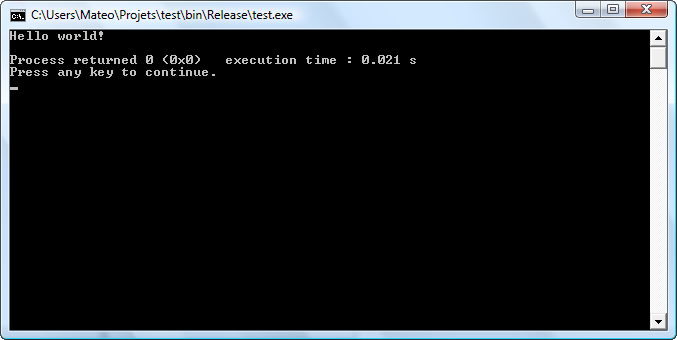
\includegraphics[width=0.8\textwidth]{Chapter_I-3_HelloWorld-run}
\end{figure}

البرنامج يُظهر
"\textenglish{Hello world!}"
 (في السطر الأوّل).\\
الأسطر الّتي أسفله تمّ توليدها من طرف
\textenglish{Code::Blocks}
 وتدلّ على أنّ البرنامج قد تمّ تشغيله بنجاح كما أنها تعطي الوقت الذي استغرقه البرنامج في التشغيل.

 سيطلب منك الضغط على إحدى المفاتيح لإغلاق النافذة. أعلم أن الأمر لم يكن ممتعا جدّا. لكنه برنامجك الأوّل، وهذه لحظة ستتذكرها طيلة حياتك ! ألا تعتقد ذلك ؟

\section{كتابة رسالة على الشاشة}

من الآن سنقوم بإدخال التعديلات على الشفرة المصدرية السابقة. مهمّتك، إن قبلتها : عرض رسالة
"\textenglish{Bonjour}"
 على الشاشة.

\begin{question}
  كيف يمكنني اختيار النص الّذي سيظهر على الشاشة ؟
\end{question}

الأمر بسيط جدا، إذا بدأت من الشفرة التي رأيناها سابقاً، فسيكون عليك استبدال
"\textenglish{Hello world!}"
 بـ"\textenglish{Bonjour}"
 في السطر الذي يستدعي
\InlineCode{printf}.

كما قلت من قبل،
\InlineCode{printf}
 هي
\textbf{تعليمة}
 وهي تعطي أمراً للحاسوب : "قم بعرض هذه الرسالة على الشاشة".\\
يجب أن تعرف أيضا أن
\InlineCode{printf}
 هي دالّة كُتِبَت من قبل من طرف مبرمجين قبلك.

\begin{question}
   أين توجد هذه الدالّة ؟ أنا لا أرى سوى الدالّة \InlineCode{main} !
\end{question}

هل تذكر هذين السطرين ؟

\begin{Csource}
#include <stdio.h>
#include <stdlib.h>
\end{Csource}

قلت لك من قبل أنهما يمكنان البرنامج من إضافة مكتبات. المكتبات في الحقيقة هي ملفّات تحوي أطنانا من الدوال جاهزة للإستخدام. هذه الملفات
(\InlineCode{stdio.h} و \InlineCode{stdlib.h})
 تحوي أغلب الدوال الأساسية التي قد نحتاجها في برنامج ما.
\InlineCode{stdio.h}
 بحد ذاته يحوي دوال تمكّن من عرض أشياء على الشاشة (مثل
 \InlineCode{printf})
 و أيضا الطلب من المستخدم إدخال شيء ما (هذه دوال سنتعرّف عليها لاحقا).

\subsection{لنقل مرحبا للسيّد}

في دالّتنا
\InlineCode{main}
نستدعي الدالّة
 \InlineCode{printf}.
 أي أن لدينا دالّة تستدعي أخرى (هنا
\InlineCode{main}
تستدعي
\InlineCode{printf}).
سترى أن هذا ما يحدث دائما في لغة
\textenglish{C}
: دالّة تحتوي تعليمات تستدعي دوال أخرى، وهكذا.

إذن، لاستدعاء دالّة يكفي كتابة اسمها متبوعا بقوسين، ثم فاصلة منقوطة.

\begin{Csource}
printf();
\end{Csource}

هذا جيد، لكنه غير كاف. يجب أن نُعلم البرنامج بما يجب أن يكتبه في الشاشة. لفعل هذا يجب أن نعطي
\InlineCode{printf}
النص المطلوب عرضه. لفعل هذا نقوم بوضع النص داخل علامات الإقتباس المزدوجة بين القوسين.\\
في حالتنا هذه سنكتب تماما :

\begin{Csource}
printf("Bonjour");
\end{Csource}

آمل ألا تكون قد نسيت رمز الفاصلة المنقوطة في النهاية، وأذكّرك أنّها مهمّة جدا لأنّها تدلّ على نهاية التعليمة.\\
هذه هي الشفرة المصدرية التي يجب أن تحصل عليها :

\begin{Csource}
#include <stdio.h>
#include <stdlib.h>

int main()
{
    printf("Bonjour");
    return 0;
}
\end{Csource}

لدينا إذن تعليمتان تطلبان من الحاسوب القيام بهذين الأمرين بهذا الترتيب :
\begin{enumerate}
  \item عرض
"\textenglish{Bonjour}"
على الشاشة.
  \item نهاية الدالّة
\InlineCode{main}
، إعادة 0. البرنامج يتوقّف.
\end{enumerate}

هذا ما يظهر على شاشتك :

\begin{figure}[H]
	\centering
	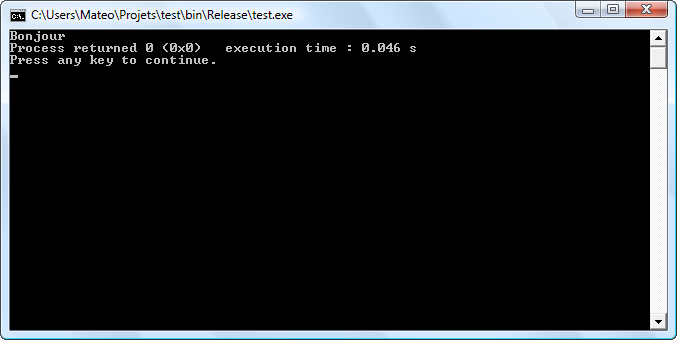
\includegraphics[width=0.8\textwidth]{Chapter_I-3_Good-Morning}
\end{figure}

كما ترى، السطر الذي يحتوي الرسالة يكون ملتصقاً قليلا بباقي النص، على خلاف ما رأيناه سابقا.\\
أحد الحلول الممكنة هو إضافة رمز للعودة إلى السطر بعد
 "\textenglish{Bonjour}"
 (كما لو أنّنا ضغطنا على المفتاح
\InlineCode{Enter}).

ولكن ضغط المفتاح
\InlineCode{Enter}
 في الشفرة المصدرية لن يعمل كما تتوقع، لهذا يجب استخدام المحارف الخاصّة
(\textenglish{Special characters}).

\subsection{المحارف الخاصّة}

المحارف أو الرموز الخاصّة هي محارف تمكّن من تعريف عودة إلى السطر، جدولة، إلخ.\\
من السهل التعرّف عليها، فهي مكوّنة من محرفين. الأوّل هو الشَرْطَةُ المائلة الخلفية 
(\textbackslash) (\textenglish{Backslash})
والثاني يكون رقما أو حرفا. إليك محرفين خاصّين قد تحتاجهما كثيرا :

\begin{itemize}
  \item \InlineCode{\textbackslash n} :
 العودة إلى السطر.
 \item \InlineCode{\textbackslash t} :
 الجدولة (فراغ كبير في نفس السطر).
\end{itemize}

في حالتنا هذه، يكفي أن نكتب
\InlineCode{\textbackslash n}
 لإنشاء العودة إلى السطر. إذن، إذا أردنا أن نضع عودة إلى السطر بعد
\textenglish{Bonjour}
، فيكفي أن نكتب :

\begin{Csource}
printf("Bonjour\n");
\end{Csource}

وسيفهم حاسوبك أنّ عليه كتابة
"\textenglish{Bonjour}"
 ويعود إلى السطر.

\begin{figure}[H]
	\centering
	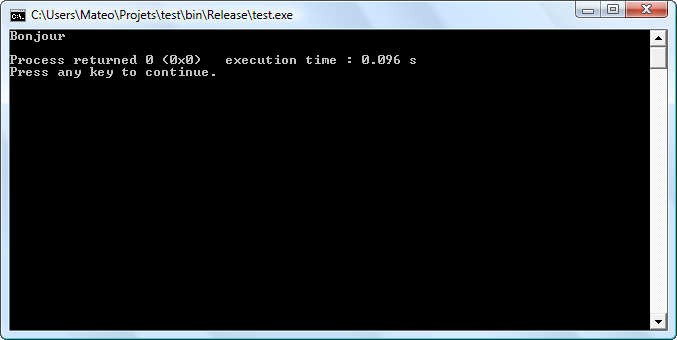
\includegraphics[width=0.8\textwidth]{Chapter_I-3_Good-Morning-backslash-n}
\end{figure}

\begin{information}
  يمكنك الكتابة بعد
\InlineCode{\textbackslash n}
بدون أيّة مشكلة. كلّ ما تكتبه بعد
\InlineCode{\textbackslash n}
 سيوضع في السطر الجديد. يمكنك إذن التدرّب على كتابة :
\InlineCode{printf("Good morning\textbackslash nGood bye\textbackslash n");}\\
و سيتمّ عرض
"\textenglish{Good morning}"
على السطر الأوّل و
"\textenglish{Good bye}"
على السطر الثاني.
\end{information}

\subsection{متلازمة \textenglish{Gérard}}

\begin{question}
  مرحبا، اسمي
\textenglish{Gérard}
و قد حاولت تعديل برنامجك ليقول
"\textenglish{Bonjour Gérard}"،
و لكنّي ألاحظ أنّ حرف
\textenglish{é}
 لا يظهر بشكل جيّد
\dots
 مالّذي عليّ فعله ؟
\end{question}

أوّلا، مرحبا بك
\textenglish{Gérard}
. هذا سؤال جيّد. لكن لديّ خبر سيّء لك. الكونسول الخاصة بـ\textenglish{Windows}
لا تمكّن من عرض الحروف الّتي تحوي علامات النطق الصوتي مثل
\textenglish{é}
، خلافا لكونسول
\textenglish{GNU/Linux}
التي تفعل. لديّ حلّان لهذه المشكلة :

\begin{itemize}
  \item \textbf{استخدم
\textenglish{GNU/Linux}}
. هذا حلّ جذريّ بعض الشيء. أحتاج إلى درس كامل لأعلّمك كيف تعمل على
\textenglish{GNU/Linux}
. إذا لم يكن لديك المستوى، إنس هذا الخيار حاليّا.
  \item \textbf{لا تستخدم الحروف الّتي تحوي علامات النطق الصوتي}.
للأسف إنّه الحل الّذي قد يكون عليك اختياره. الكونسول الخاصة بـ\textenglish{Windows}
لها عيوبها. يجب عليك التعوّد على عدم كتابة مثل هذه الحروف. لكن مستقبلا قد تنشئ برامج بنوافذ ولن تعاني من هذا المشكل. لذلك أنصحك بالصبر على هذه المشكلة حاليّا، فبرامجك المستقبلية "الاحترافية" لن يكون فيها هذا المشكل.
\end{itemize}

لكيلا تنزعج، يمكنك الكتابة دون استخدام الحروف التي تملك علامات النطق الصوتي :

\begin{Csource}
printf("Bonjour Gerard\n");
\end{Csource}

نشكر صديقنا
\textenglish{Gérard}
لتنبيهنا على هذه المشكلة !

\section{التعليقات، مهمّة جدا !}

قبل ختم هذا الفصل الأوّل "الحقيقي" في البرمجة، يجب أن أعرّفك على
\textbf{التعليقات}
(\textenglish{Comments})
. أيّا كانت لغة البرمجة الّتي تستخدمها، ستكون لديك القدرة على إضافة التعليقات للشفرة المصدرية الخاصة بك.

ولكن ما الذي يعنيه "التعليق"؟\\
هذا يعني إمكانية وضع نصّ في وسط برنامجك لشرح دوره، مثلاً : ما الذي يفعله هذا السطر، إلخ. هذا بالفعل أمر ضروريّ، لأنّه حتّى لو كنت عبقرياً في البرمجة، ستكون بحاجة إلى وضع ملاحظات هنا وهناك. هذا يمكنك من :

\begin{itemize}
  \item العثور على ما تبحث عنه بسهولة في الشفرة المصدرية عندما تعود إليه بعد مدّة. من الطبيعيّ أن ننسى كيف تعمل البرامج الّتي كتبناها بعد مدّة. إن توقّفت عن البرمجة لأيّام ثمّ عدت فستكون بحاجة إلى التعليقات لإيجاد ما تريد في شفرة كبيرة جدّا.
  \item إذا أعطيت مشروعك لأحد غيرك (وهو لا يعرف شيئا عن الشفرة المصدرية الخاصة بك)، فالتعليقات تمكّنه من التآلف مع مشروعك بسرعة.
  \item وأخيرا، ستسمح لي بإضافة شروحات وملاحظات حول الشفرة المصدرية في هذه الدروس. وهذا سيفيدك في فهم ما الذي يعنيه كلّ سطر.
\end{itemize}

توجد طريقتان لإضافة تعليق. وهذا يعتمد على طول التعليق المراد إدراجه :

\begin{itemize}
  \item إذا كان تعليقك
\textbf{قصيرا}
: فيمكن كتابته على سطر واحد، ولا يحتوي سوى كلمات قليلة. في هذه الحالة، عليك كتابة شرطتين مائلتين
(\InlineCode{//})
متبوعين بتعليقك. على سبيل المثال :

\begin{Csource}
// This is a comment.
\end{Csource}

بإمكانك إضافة تعليق وحده على السطر، أو على يمين تعليمة معينة. وهذا أمر مهمّ جدّا، لأنّ بهذه الطريقة يمكننا تحديد ما الذي يعنيه السطر الّذي كُتب بجانبه. مثال :

\begin{Csource}
printf("Bonjour"); // This instruction displays 'Bonjour' on the screen
\end{Csource}

  \item  إذا كان تعليقك
\textbf{طويلا}:
لديك الكثير لتقوله، تريد كتابة الكثير من الجمل على كثير من الأسطر. في هذه الحالة، يجب عليك كتابة شفرة تشير إلى "بداية التعليق" وأخرى تشير إلى "نهاية التعليق":

  \begin{itemize}
    \item لبدء التعليق : أكتب شرطة مائلة متبوعة بنجمة 
    (\InlineCode{/*}).
    \item لإنهاء التعليق : أكتب نجمة متبوعة بشرطة مائلة 
    (\InlineCode{*/}).
  \end{itemize}

  يمكنك كتابة هذا على سبيل المثال :
  
  \begin{Csource}
/* This is
a comment
written on several lines */
  \end{Csource}
\end{itemize}
فلنعد إلى الشفرة المصدرية التي تُظهر
"\textenglish{Bonjour}"
على الشاشة ونضيف إليها بعض التعليقات للتدرّب :

\begin{Csource}
/*
Below, the directives of preprocessor.
These lines allow you to add files to your program,
files that we call libraries. Thanks to these libraries, we are ready to use functions for display.
for example, a message on screen.
*/

#include <stdio.h>
#include <stdlib.h>

/*
Following, you have the principal function of the program, called main.
All programs start with this function.
Here, all what does my function is displaying "Bonjour" on the screen.
*/

int main()
{
  printf("Bonjour"); // This instruction displays 'Bonjour' on the screen
  return 0;          // The program returns 0 then it stops.
}
\end{Csource}

هذا هو برنامجنا مع إضافة بعض التعليقات، نعم هو يبدو أكبر نوعا ما، لكنّه في الحقيقة مكافئ للبرنامج السابق. عند الترجمة، كلّ التعليقات يتمّ تجاهلها من طرف المترجم. هذه التعليقات لا تظهر في البرنامج النهائي، فهي تصلح فقط للمبرمجين.

عادة لا نقوم بوضع تعليق لكلّ سطر. لقد قلت وأكرر أنّه من المهم وضع التعليقات في الشفرة المصدرية، لكن يجب عليك معرفة القدر اللازم من التعليقات الواجب وضعه، وضع تعليق في كلّ سطر قد لا يفيد في شيء، بل يضيّع الوقت فقط. مثلا، أنت تعرف أن وظيفة
\InlineCode{printf}
هي عرض نصّ على الشاشة، فلا حاجة لوضع تعليق يشرح ذلك في كلّ مرّة.

من الأحسن التعليق عن عدد من الأسطر دفعة واحدة. هذا يفيد في ذكر وظيفة مجموعة من التعليمات المتتابعة. فيما بعد إن أراد المبرمج إضافة مزيد من التفاصيل في تعليماته، فسيكون بمستوى ذكاء يسمح له بفعل ذلك.

\textbf{تذكر إذن}:
يجب أن تكون التعليقات لإرشاد المبرمج في شفرته المصدرية. حاول التعليق عن مجموعة من الأسطر دفعة واحدة بدل التعليق عن كلّ سطر على حدة.

وإليك هذه المقولة من
\textenglish{IBM} :

\begin{center}
  \itshape\Large
  'إذا قرأت التعليقات الموجودة في برنامج و لم تفهم مبدأ عمله، قم برميه !'
\end{center}

\section*{ملخّص}

\begin{itemize}
  \item البرامج يمكنها التفاعل مع المستخدم عن طريق الكونسول أو عن طريق النافذة.
  \item من السهل على المبرمج في برامجه الأولى استخدام
\textbf{الكونسول}،
رغم أنّ هذه قد تكون غير محبوبة لدى المبتدئ، فهذا لا يمنع من استخدام النوافذ في الجزء الثالث من هذا الكتاب.
  \item البرنامج يتكوّن من
\textbf{تعليمات}
 تنتهي دائما بفاصلة منقوطة.
  \item الدالة
\InlineCode{main}
 (التي تعني الرئيسيّة) هي الدالة الّتي يبدأ بها تنفيذ البرنامج. إنّها الدالة الوحيدة الإجبارية في البرنامج، لا يمكن لأي برنامج أن يُترجم بدونها.
 \item \InlineCode{printf}
 هي دالة تمكننا من عرض رسالة على الشاشة.
 \item \InlineCode{printf}
موجودة في
\textbf{مكتبة}
 تحتوي على كثير من الدوال الأخرى الجاهزة للاستخدام.
\end{itemize}

  \chapter{عالم المتغيّرات}

تعلّمت كيفية إظهار نصّ على الشاشة. جيد، لكنّ هذا ليس شيئا مهماً. هذا لأنك لا تعرف بعد ما يدعى بـ
\underline{المتغيّرات}
(\textenglish{Variables})
في البرمجة.

فائدة هذه المتغيرات هي تمكين الحاسوب من حفظ أعداد في الذاكرة. سنبدأ ببعض الشرح حول ذاكرة الحاسوب وكيفيّة عملها. قد يبدو هذا بسيطا جدّا للبعض، لكنّي أفترض أنّك لا تعرف شيئا عن ذاكرة الحاسوب.

\section{أمر متعلق بالذاكرة}
ما سأعلمك في هذا الدرس هو أمر له علاقة مباشرة بذاكرة حاسوبك.

كل إنسان حيّ له ذاكرة. الأمر عينه بالنسبة للحاسوب، لكن الحاسوب له أنواع عديدة من الذاكرة.

\begin{question}
  لم يملك الحاسوب أنواع عديدة من الذاكرة، واحدة يمكنها أن تكفي، أليس الأمر كذلك؟
\end{question}
كلّا: المشكلة أننا نحتاج ذاكرة سريعة (لاسترجاع المعلومات بسرعة) وفي نفس الوقت كبيرة (لحفظ بيانات كثيرة) قد تضحك إن أخبرتك أننا حتى اليوم لم نتمكن من صنع ذاكرة بهذه المواصفات. أو بالأحرى الذاكرة السريعة باهظة الثمن لذلك لا يتم إنتاج الكثير منها.

لذلك نجد في الحواسيب الحديثة ذاكرة سريعة جدا لكنها ليس ذات سعة كبيرة، وأخرى ذات سعة كبيرة جدّا لكنها غير سريعة.

\subsection{الأنواع المختلفة من الذاكرة}
كي أوضح لك الصورة أكثر، إليك أنواع الذاكرة الموجودة في الحاسوب، من الأسرع إلى الأبطأ:
\begin{enumerate}
  \item السجلات (
\textenglish{Registers}
): ذاكرة سريعة جدّا، موجودة داخل المعالج.
  \item ذاكرة التخبئة (
\textenglish{Cache memory}
): تمثل همزة وصل بين السجلات والذاكرة الحية.
  \item ذاكرة الوصول العشوائي (
\textenglish{Random access memory}
): وهي الذاكرة التي نستخدمها كثيرا، وتدعى اختصارا
\textenglish{RAM}.
  \item القرص الصلب (
\textenglish{Hard disk}
): والذي تعرفه بالطبع، نستعمله لحفظ الملفات.
\end{enumerate}
كما قلت لك، لقد رتبتها من الأسرع (السجلات) إلى الأبطأ (القرص الصلب)، وإن كنت قد تابعت جيدا فقد فهمت أن الذاكرة الأصغر هي الأسرع والأبطأ هي الأكبر.\\
السجلات لا تسع إلا لحمل بضعة أعداد أما القرص الصلب فيمكنه تخزين ملفات ضخمة.

\begin{information}
   عندما أقول ذاكرة بطيئة فهذا بالنسبة لحاسوبك، ففي نظر الحاسوب استغراق 8 ميلي ثانية للوصول إلى القرص الصلب يعتبر زمنا طويلا جدّا!
\end{information}

ما الذي يجب أن أتذكره من كل هذا؟\\
أردت أن أخبرك أننا في الدروس القادمة سوف نستخدم ذاكرة الوصول العشوائي كثيرا. سنتعلم أيضا كيفية القراءة والكتابة في الملفات على القرص الصلب (ليس الآن، لا يزال الوقت مبكّرا على هذا). أمّا بخصوص السجلّات وذاكرة التخبئة فلن نتعامل معهما مطلقا، فالحاسوب هو من سيهتم بأمرهما.

\begin{information}
  في لغات البرمجة منخفضة المستوى، كلغة التجميع (
\textenglish{Assembly language}
) نتعامل مباشرة مع السجلّات، لقد درستها، ويمكنني أن أقول لك أن القيام بعملية ضرب بسيطة يتطلب مجهودا! لحسن الحظ ففي لغة
\textenglish{C}
 (وفي أغلب اللغات الأخرى) الأمر أسهل من ذلك بكثير.
\end{information}

يجب إضافة شيء مهمّ آخر: القرص الصلب هو الوحيد الذي يمكنه حفظ المعلومات بشكل دائم.
\textbf{كل أنواع الذاكرات الأخرى مؤقتة، فبمجرد إطفاء الحاسوب تفقد كل محتواها}!

لحسن الحظ فعند إعادة تشغيل الحاسوب يقوم القرص الصلب بتذكيرها بمحتواها.

\subsection{صورة لذاكرة الوصول العشوائي}
نظرا لأننا سنستعمل ذاكرة الوصول العشوائي خلال لحظات، فمن الأفضل أن أريها لكم (مؤطر بالأحمر):
\Picture{Chapter_I-4_Computer}
لا أطلب منك معرفة كيفية عملها، لكن أردت فقط أن أريك مكانها داخل جهازك. وهذه صورة مقربة لإحدى أشرطتها:
\Picture{Chapter_I-4_RAM}
وهي تدعى اختصارا
\textbf{\textenglish{RAM}}
، لذلك لا تحتر إن سميتها هكذا لاحقا. بالنسبة للذاكرات الأخرى (السجلات والتخبئة) فهي صغيرة لدرجة أنه لا يمكن رؤيتها بالعين المجرّدة.

\subsection{مخطط ذاكرة الوصول العشوائي}
عرض المزيد من الصور لن يفيدك كثيرا، لكن يجب عليك فهم كيف تعمل من الداخل، لذلك سأقدم لك هذا المخطط البسيط الذي يمثل هندسة ذاكرة الوصول العشوائي:
\Picture{Chapter_I-4_RAM-Schema}

كما ترى، يمكننا أن نميز عمودين:
\begin{itemize}
  \item هناك
\textbf{العناوين}
: هي أعداد تسمح للحاسوب بتحديد موضع القيم في الـ
\textenglish{RAM}
. نبدأ بالعنوان 0 وننتهي بالعنوان 3,448,765,900,126 وبعض الأجزاء. لا أعلم بالضبط كم عدد العناوين الموجودة في الـ
\textenglish{RAM}
، لكني أعرف أنها كثيرة جدا. إضافة إلى ذلك، هذا أمر يتعلق بكمية الذاكرة الموجودة في جهازك، فكلما زادت الذاكرة زادت معها العناوين وصار بإمكاننا تخزين معلومات أكثر.
  \item عند كل عنوان يمكننا تخزين
\textbf{قيمة}
(عدد). حاسوبك يقوم بتخزين هذه الأعداد في ذاكرة الوصول العشوائي لكي يتمكن من تذكرها. ولا يمكننا تخزين سوى عدد واحد عند كل عنوان.
\end{itemize}

لا يمكن للذاكرة الحية تخزين شيء سوى الأعداد.

\begin{question}
  لكن كيف يمكننا تخزين الكلمات؟
\end{question}

سؤال جيد. في الواقع حتى الحروف ليست سوى أعداد في نظر الحاسوب! الجملة هي مجرد تتابع لأعداد.\\
يوجد جدول يوافق بين الأعداد والحروف، جدول يقول مثلا بأن العدد 67 يوافق الحرف
\textenglish{Y}
. لن أدخل في التفاصيل أكثر، ستكون لنا فرصة للرجوع إلى هذا لاحقا.

فلنعد إلى مخططنا، الأمور بسيطة جدا: إذا أراد الحاسوب تذكر العدد 5 (الذي قد يمثل عدد الأرواح المتبقية لشخصية في لعبة) فسوف يضعه في مكان ما في الذاكرة أين يتوفر مكان شاغر ويحفظ العنوان الموافق (مثلا 3,062,199,902). لاحقا، عندما يريد معرفة هذا العدد فسيذهب إلى خانة الذاكرة التي تحمل العنوان رقم 3,062,199,902 وسيجد القيمة 5.

هذه آلية عمل الذاكرة بشكل عام. قد يكون الأمر لا زال غامضا في ذهنك حاليا (ما فائدة تخزين عدد إن كان علينا تذكر عنوانه بدلا من ذلك؟) لكن كل شيء سيتضح مع بقية الدروس، أنا أعدك!

\section{التصريح عن متغير}
صدّقني هذه المقدّمة القصيرة عن الذاكرة ستكون مهمّة أكثر مما تعتقد. الآن يمكننا العودة إلى البرمجة.

إذن، ما هو
\underline{المتغير}
(\textenglish{Variable}) ؟\\
إنه معلومة صغيرة نخزنها مؤقتا في الذاكرة الحية. ببساطة يمكننا القول إن المتغير هو قيمة يمكن أن تتغير أثناء اشتغال البرنامج. مثلا عددنا 5 الذي ذكرناه سابقا يمكن أن يتناقص بمرور الزمن. إذا وصل إلى العدد 0 فسنعرف أن اللاعب قد خسر.

في برامجنا سيكون هناك الكثير من المتغيرات. ستراها في كلّ مكان.

في لغة السي، المتغير يتميز بشيئين:
\begin{itemize}
  \item \underline{قيمة}
: هو العدد الذي يحويه، 5 مثلا.
  \item \underline{اسم}
: وهو الذي يمكننا من معرفة المتغيّر. في البرمجة لن يكون علينا تذكّر عناوين الذاكرة. بدلا من ذلك علينا فقط استخدام أسماء المتغيرات. المترجم هو من سيقوم بتحويل الأسماء إلى عناوين.
\end{itemize}

\subsection{إعطاء اسم للمتغير}
في لغة البرمجة
\textenglish{C}
كل متغير يجب أن يملك اسما خاصا به. ومن أجل متغيرنا الذي يحوي عدد الأرواح المتبقية للاعب يمكننا أن نسميه
"\textenglish{Number of lives}"
أو شيء من هذا القبيل.

للأسف توجد بعض الشروط، لا يمكنك تسمية المتغير كيفما شئت:
\begin{itemize}
  \item لا يجب أن يحتوي الاسم سوى على الحروف الصغيرة والكبيرة والأرقام
(\InlineCode{abcABC012}).
  \item يجب أن يبدأ الاسم بحرف.
  \item المسافات ممنوعة. بدلا من ذلك يمكننا استخدام الحرف المعروف باسم
\textenglish{underscore}
 (\InlineCode{\_}).
إنه الحرف الخاص الوحيد غير الحروف والأرقام الذي يمكن استعماله في اسم متغير.
  \item لا يمكنك استخدام حروف غير الحروف الإنجليزية.
\end{itemize}

وأخيرا يجب أن تعرف أن لغة
\textenglish{C}
 تفرّق بين الحروف الصغيرة والكبيرة. ولثقافتك، نقول إن
\textenglish{C}
 حساسة لحالة الأحرف
(\textenglish{Case sensitive}).
كمثال، الأسماء
\InlineCode{width}
 أو
\InlineCode{WIDTH}
 أو
\InlineCode{WiDth}
تعتبر أسماء متغيرات مختلفة، حتى لو كانت تعني لنا الأمر نفسه.

هذه أمثلة عن أسماء متغيرات صالحة:
\InlineCode{numberOfLives}،
\InlineCode{name}،
\InlineCode{surname}،
\InlineCode{phone\_number}،
\InlineCode{phoneNumber}.

لكل مبرمج طريقة خاصة في كتابة أسماء المتغيرات. خلال هذا الدرس سأريك طريقتي:
\begin{itemize}
  \item أبدأ دائما بحرف صغير.
  \item إن كان في الاسم أكثر من كلمة أضع حرف كبيرا في بداية كلّ كلمة.
\end{itemize}

أطلب منك كتابة أسماء متغيراتك بنفس الطريقة التي أتبعها، هذا لكي نكون على تفاهم.

\begin{critical}
  أيّا كان اختيارك، فعليك دائما إعطاء أسماء واضحة لمتغيراتك. كان بإمكاننا اختصار
\InlineCode{numberOfLives}
إلى
\InlineCode{nol}
مثلا. هذا أقصر في الكتابة، لكنه أقل وضوحا عندما تعيد قراءة الشفرة المصدرية. فأنصحك بإعطاء أسماء أطول لمتغيراتك إن كان ذلك يحسّن فهمها.
\end{critical}

\subsection{أنواع المتغيرات}
حاسوبنا كما نعلم ليس سوى آلة كبيرة جدا للحساب. لا يجيد التعامل سوى مع الأعداد. لكن يوجد أنواع كثيرة من الأعداد:
\begin{itemize}
  \item الأعداد الصحيحة الموجبة (الطبيعية) مثل :45، 398، 7650.
  \item الأعداد العشرية، أي التي تحوي فاصلة عشرية: 75.909، 1.7741، 9810.7.
  \item الأعداد الصحيحة السالبة: -87، -916.
  \item الأعداد العشرية السالبة: -76.9، -100.11.
\end{itemize}

حاسوبك المسكين بحاجة للمساعدة! عندما تطلب منه تخزين عدد، يجب أن تذكر له نوعه. هذا ليس لأنّه لا يمكنه التعرف عليه تلقائيّا، ولكن للتنظيم ولعدم أخذ كميات كبيرة من الذاكرة بدون فائدة.

عندما تصرّح عن متغيّر فسيكون عليك تحديد نوعه. إليك أنواع المتغيرات الأساسية في لغة \textenglish{C}:

\begin{Table}{3} % The number of columns is required (here is 3)
  النوع & الحد الأدنى & الحد الأقصى\\
  \LR{\ttfamily signed char} & $-128$ & $127$ \\
  \LR{\ttfamily int} & $-32,768$ & $32,767$ \\
  \LR{\ttfamily long} & $-2147483648$ & $2147483647$ \\
  \LR{\ttfamily float} & $-1 \times 10^{37}$ & $1 \times 10^{37}-1$\\
  \LR{\ttfamily double} & $-1 \times 10^{37}$ & $1 \times 10^{37}-1$\\
\end{Table}

\begin{warning}
  القيم المعروضة هنا تمثل الحد الأدنى المضمون من طرف اللغة. في الحقيقة قد تتمكن من تخزين أعداد أكبر من هذه. في كلّ الأحوال من المستحسن تذكّر هذه القيم عندما تختار نوع متغيراتك.
\end{warning}

\begin{information}
  للعلم أنّي لم أعرض جميع الأنواع هنا، بل الأساسية منها فقط.
\end{information}

الأنواع الثلاثة الأولى
(\InlineCode{char}، \InlineCode{int}، \InlineCode{long})
تسمح يتخزين الأعداد الصحيحة (1،2،3،4،...).\\
النوعان الأخيران
(\InlineCode{float}، \InlineCode{double})
يسمحان بتخزين الأعداد العشرية (13.8, 16.911…).

سترى أنّنا نتعامل من الأعداد الصحيحة معظم الوقت لأنّها سهلة الإستخدام.

\begin{critical}
  احذر في الأعداد العشرية من استخدام الفاصلة، حاسوبك لا يستخدم سوى النقطة. لذلك لا تكتب
$54,9$
 بدل
$54.9$!
\end{critical}

هذا ليس كلّ شيء، توجد أنواع أخرى تعرف بـ
\InlineCode{unsigned}
 (عديمة الإشارة) تصلح لتخزين الأعداد الموجبة فقط. يجب إضافة كلمة
\InlineCode{unsigned}
إلى النوع لاستخدامها.

\begin{Table*}{2}
  \LR{\ttfamily unsigned char} & من
$0$
 إلى
$255$ \\
  \LR{\ttfamily unsigned int} & من
$0$
إلى
$65,535$ \\
  \LR{\ttfamily unsigned int} & من
$0$
إلى
$4,294,967,295$\\
\end{Table*}

كما ترى، مشكلة الأنواع عديمة الإشارة هي عدم القدرة على تخزين الأعداد السالبة، لكن الشيء الإيجابي هي أنّها توفّر لنا ضعف حجم التخزين لكلّ نوع موافق (مثلا
\InlineCode{signed char}
يتوقّف عند 127، بينما
\InlineCode{unsigned char}
يمتد إلى 255.

\begin{information}
  تلاحظون أنّ النوع
\InlineCode{char}
قد تمّ إدراجه إمّا مع الكلمة المفتاحية
\InlineCode{signed}
،أو مع الكلمة المفتاحية
\InlineCode{unsigned}
لكن لا يوضع وحده أبدا. السبب بسيط: هذا النوع يمكن أن يكون بإشارة أو بدون إشارة حسب الحواسيب. لذلك أنصحكم بتحديد أي واحد منهما تريدون حسب نوع القيمة المراد تخزينها.
\end{information}

\begin{question}
  لم توجد ثلاثة أنواع من المتغيرات الصحيحة ؟ ألا يكفي نوع واحد ؟
\end{question}

بلى، و لكن إنشاء أنواع متعدّدة هدفه الاقتصاد من استهلاك الذاكرة. فعندما نطلب من الحاسوب حجز مساحة لمتغيّر من نوع
\InlineCode{char}
فهذا سيكون أقل من المساحة المستهلكة لو إخترنا متغيّرا من نوع
\InlineCode{int}.

كان هذا مهمّا جدّا عندما كانت الحواسيب محدودة الذاكرة. أمّا اليوم فحواسيبنا بها ذاكرات كبيرة جدّا فلم يعد هذا يمثّل مشكلة. إذا احترت أيّ واحد من الأنواع تستخدم، فاختر
\InlineCode{int}
للأعداد الصحيحة (أو
\InlineCode{double}
للعشرية).

باختصار، نقوم بالتفريق خاصّة بين الأعداد الصحيحة و العشريّة
\begin{itemize}
  \item بالنسبة للأعداد الصحيحة، نستعمل عادة
\InlineCode{int}.
  \item بالنسبة للأعداد العشريّة نستعمل عادة
\InlineCode{double}.
\end{itemize}

\subsection{التصريح عن متغيّر}
ها قد بدأنا. الآن سنقوم بإنشاء برنامج كونسول نسميه "\textenglish{variables}".\\
 سنتعلم كيف نصرّح عن متغيّر، أي
 \textbf{الطلب من الحاسوب إذنا باستخدام شيء من ذاكرة الوصول العشوائي}.

 التصريح سيكون سهلا الآن، يجب علينا فقط أن نتّبع الترتيب التالي :
 \begin{enumerate}
   \item نحدّد نوع المتغيّر المراد إنشائه.
   \item نترك فراغا.
   \item نحدد اسم المتغيّر.
   \item و أخيرا، يجب ألاّ ننسى أبدا وضع الفاصلة المنقوطة.
 \end{enumerate}

 مثلا، إذا أردنا إنشاء المتغيّر
\InlineCode{numberOfLives}
 من نوع
\InlineCode{int}
سنكتب السطر التالي :
\begin{Csource}
int numberOfLives;
\end{Csource}

هذا كل ما في الأمر، وإليك بعض الأمثلة الغبيّة لملاحظة الشكل:
\begin{Csource}
int mathMark;
double moneySumReceived;
unsigned int numberOfReadersWhoAreReadingALongVariableName;
\end{Csource}
حسنا، أعتقد أنّك فهمت المبدأ الآن !

ما فعلناه للتو يسمّى
\underline{تصريحا عن متغيّر}
(\textenglish{Declaring a variable})
(هذا مصطلح يجب حفظه). يمكنك وضع التصريحات في بدايات الدوال. و بما أن لدينا دالّة وحيدة فقط
(الدالة
\InlineCode{main})
فسنصرّح المتغيّر هكذا :
\begin{Csource}
#include <stdio.h>
#include <stdlib.h>

int main(int argc, char *argv[]) // Equivalent to int main()
{
  int numberOfLives;

  return 0;
}
\end{Csource}
إن قمتم بتشغيل البرنامج فستلاحظ بدهشة ... أنّه لا يقوم بشيء.

\subsection{بعض التوضيحات}
في الواقع، هناك أشياء تحدث، لكنّك لا تراها. عندما يصل البرنامج إلى سطر التصريح عن المتغيّر فإنّه يطلب من الحاسوب بهدوء أن يعطيه شيئا من ذاكرة الوصول العشوائي.\\
إن تم كلّ شيء على أحسن حال (و هذا ما يقع في غالب الأحيان) فإن الحاسوب يوافق على هذا الطلب.
المشكل الوحيد الذي يمكن أن يقع هو امتلاء الذاكرة، لكنّ هذا أمر نادر الحدوث، من الذي سيملؤ الذاكرة بمتغيرات
\InlineCode{int}
 ؟

لذلك كن متيقناً أنه سوف يتم إنشاء المتغيرات بنجاح.

\begin{information}
  معلومة صغيرة : إن كان لديك عدد من المتغيّرات بنفس النوع تريد التصريح عنها، فمن غير الضروري كتابة سطر لكلّ متغيّر. يكفي فصل أسماء المتغيّرات عن بعضها بفواصل على نفس السطر، مثلا :
\InlineCode{int numberOfLives, level, playerAge;}.
هذا ينشئ ثلاثة متغيّرات أسماؤها على التوالي :
\InlineCode{numberOfLives}، \InlineCode{level}
و
\InlineCode{playerAge}.
\end{information}

و الآن يجب علينا إعطاء قيمة للمتغيّر الذي أنشأناه.

\subsection{إسناد قيمة إلى متغيّر}
هذا أمر سهل للغاية فإن أردنا أن نعطي قيمة لمتغيرنا
\InlineCode{numberOfLives}
فيكمننا ببساطة كتابة هذا
\begin{Csource}
numberOfLives = 5;
\end{Csource}
لن نفعل شيئا بعد هذا. ستضع إسم المتغير، إشارة تساوي ، بعدها القيمة التي تريد أن تضعها بالداخل، في هذه الحالة سنعطي القيمة 5 للمتغير
\InlineCode{numberOfLives}
. برنامجنا الكامل سيكون هكذا :
\begin{Csource}
#include <stdio.h>
#include <stdlib.h>

int main(int argc, char *argv[]) // Equivalent to int main()
{
  int numberOfLives;
  numberOfLives = 5;

  return 0;
}
\end{Csource}
هنا أيضا لا شيء يُعرض على الشاشة، كلّ شيء يحدث في الذاكرة.\\
في أعماق الحاسوب هناك خانة ذاكرة تأخذ القيمة 5. أليس شيئا رائعا ؟

يمكننا أن نستمتع بتغيير القيمة :
\begin{Csource}
int numberOfLives;
numberOfLives = 5;
numberOfLives = 4;
numberOfLives = 3;
\end{Csource}
في هذا المثال، المتغير سيأخذ القيمة 5 ثم 4 ثم 3. و بما أنّ الحاسوب سريع جدّا ففي أقلّ من رمشة عين يأخذ المتغيّر القيم 5 ثمّ 4 ثمّ 3 ثمّ ينتهي البرنامج.

\subsection{قيمة متغيّر جديد}
هناك سؤال مهمّ يجب أن أطرحه عليك :
\begin{question}
  عند التصريح عن متغيّر، أيّ قيمة تكون فيه ؟
\end{question}
عندما يقرأ الحاسوب هذا السطر
\begin{Csource}
int numberOfLives;
\end{Csource}
فسيحجز مكانا في الذاكرة لهذا المتغيّر، لكن ما هي قيمته في هذه اللحظة ؟\\
هل يملك قيمة افتراضيّة ؟ (0 مثلا).

الجواب هو لا، لا و لا ثمّ لا ! لا توجد قيمة افتراضيّة. المكان محجوز لكنّ القيمة لا تتغيّر. لا يتمّ حذف ما يوجد في خانة الذاكرة. ستكون قيمة متغيّرك هي نفس القيمة التي كانت موجودة من قبل في تلك الخانة، و
\textbf{يمكن أن تكون أيّ شيء} !

إن لم يتم تغيير هذا المكان من الذاكرة من قبل، فقد تكون قيمته 0، لكنّ هذا ليس مؤكّدا، قد يأخد متغيّرك القيمة 363 أو 18، و هذا يدلّ على بقايا برنامج قد استخدم هذه الخانة من قبل.\\
و لهذا كي لا تعترضنا المشاكل لاحقا يجب تهيئة المتغير عند التصريح عنه، في لغة
\textenglish{C}
هذا أمر ممكن حيث أنّ كل ما يجب القيام به هو الدمج بين التصريح و تعيين قيمة المتغير في نفس التعليمة كالتالي :
\begin{Csource}
int numberOfLives = 5;
\end{Csource}
هنا يتمّ  التصريح عن المتغيّر ثمّ إسناد قيمة 5 له بطريقة مباشرة.\\
الشيء الإيجابي هنا أننا متأكدون من أنّ المتغيّر يحمل القيمة 5 مبدئيّا.

\subsection{الثوابت}
قد نريد أحيانا إنشاء متغيّر يحمل قيمة ثابتة طوال وقت تشغيل البرنامج. هذا يعني أنّه بمجرّد التصريح عنه، فإنّه يحافظ على قيمته و لا يمكن لأحد تغيير قيمته التي يحويها.

هذا النوع الخاص من المتغيّرات يسمى الثوابت (\textenglish{Constants})، طبعا هذا لأنّ قيمتها تبقى ثابتة.

للتصريح عن ثابت، تكفي إضافة كلمة
\InlineCode{const}
قبل نوع المتغيّر. و لكن يجب إعطاء الثابت قيمة بمجرّد التصريح عنه، لأنّه لاحقا سيكون الوقت متأخّرا و لن نتمكّن من تغيير قيمته.

مثال على التصريح بثابت :
\begin{Csource}
const int INITIAL_NUMBER_OF_LIVES = 5;
\end{Csource}
\begin{information}
  ليس من الضروري أن يكون اسم الثابت مكوّنا من أحرف كبيرة فقط، لكنّ هذا يساعدنا على التفريق بينها و بين المتغيّرات. لاحظ أيضا أننا نستخدم الرمز
\_
 بدلا من الفراغ.
\end{information}
بغضّ النظر عن هذا، الثابت يستعمل بشكل عادي كالمتغير ، يمكنك عرض قيمته إن أردت. الفرق الوحيد هو أنّه إذا حاولت تغيير قيمة الثابت في برنامجك فسينبّهك المترجم إلى وجود خطأ.

أخطاء الترجمة تعرض أسفل الشاشة (في المكان الذي أسميه "منطقة الموت" هل تتذكر ؟)، في هذه الحالة سيقوم المترجم بعرض رسالة تشبه التالي :\\
\InlineCode{[Warning] assignment of read-only variable 'INITIAL\_NUMBER\_OF\_LIVES'}

\section{عرض محتوى متغير}
نحن نعرف كيف نعرض نصّا على الشاشة باستخدام الدالة
\InlineCode{printf}.\\
الآن سنتعلم كيف نعرض القيمة الخاصة بالمتغير باسخدام نفس الدالة.

سنستخدم الدالة
\InlineCode{printf}
بنفس الطريقة، باستثناء أننا سنقوم بإضافة رمز خاص في المكان الّذي نريد عرض قيمة المتغيّر فيه. مثلا :
\begin{Csource}
printf("You have %d lives left");
\end{Csource}
هذا الرمز الخاص ما هو إلّا
\InlineCode{\%}
 متبوعا بحرف (
\InlineCode{'d'}
في هذا المثال). هذا الحرف يبيّن ما الذي سنقوم بعرضه.
\InlineCode{'d'}
تعني أننا سنعرض قيمة متغيّر من نوع
\InlineCode{int}.\\
توجد حروف أخرى عديدة، لكن من أجل التبسيط فسنكتفي بهذه :
\begin{Table}{2}
الشكل & النوع المنتظر\\
\LR{\ttfamily \%d} & \LR{\ttfamily int}\\
\LR{\ttfamily \%ld} & \LR{\ttfamily long}\\
\LR{\ttfamily \%f} & \LR{\ttfamily float}\\
\LR{\ttfamily \%f} & \LR{\ttfamily double}\\
\end{Table}
\begin{information}
  لاحظوا أنّ الشكل المستخدم لعرض
\InlineCode{float}
و
\InlineCode{double}
هو نفسه.
\end{information}
سأعلّمك رموزا أخرى في الوقت المناسب، حاليّا تذكّر هذه فقط.

شارفنا على الإنتهاء. حددنا موضع كتابة عدد صحيح، لكننا لم نذكر ما هو ! يجب علينا أن نحدد للدالة
\InlineCode{printf}
المتغيّر الذي نريد عرض قيمته.\\
لفعل ذلك، أكتب اسم المتغيّر بعد علامات الاقتباس بعد وضع فاصلة :
\begin{Csource}
printf("You have %d lives left", numberOfLives);
\end{Csource}
\InlineCode{\%d}
 سيتمّ استبداله بقيمة المتغيّر المكتوب بعد الفاصلة، أي
\InlineCode{numberOfLives}.\\
فلنجرّب هذا في برنامج :
\begin{Csource}
#include <stdio.h>
#include <stdlib.h>

int main(int argc, char *argv[])
{
  int numberOfLives = 5; // The player has 5 lives in the beginning.

  printf("You have %d lives left\n", numberOfLives);
  printf("**** B A M ****\n"); // A big blow on his head.
  numberOfLives = 4; // Life lost
  printf("Sorry, only %d lives are remaining now !\n\n", numberOfLives);

  return 0;
}
\end{Csource}
يمكن أن يكون البرنامج قاعدة للعبة فيديو (ينقصه الخيال فقط).\\
هذا البرنامج يعرض على الشاشة :
\begin{Console}
You have 5 lives left
**** B A M ****
Sorry, only 4 lives are remaining now !

\end{Console}
يجب أن تفهم ما الذي يحدث في البرنامج :
\begin{enumerate}
  \item في البداية يملك اللاعب 5 أرواح، نعرض هذا في
\InlineCode{printf}.
  \item  بعدها يتلقى اللاعب ضربة على رأسه (في مكان
\textenglish{BAM}).
  \item بعدها لا يبقى له سوى 4 أرواح، نعرض هذا أيضا باستخدام
\InlineCode{printf}.
\end{enumerate}
كان ذلك سهلا !

\subsection{عرض عدّة متغيّرات باستخدام
\texttt{printf}
واحدة
}
يمكن عرض قيم متغيرات عديدة بنفس الدالة
\InlineCode{printf}.
يكفي فقط أن تضع
\InlineCode{\%d}
أو
\InlineCode{\%f}
 في الأمكنة المناسبة، ثم تحديد المتغيّرات الموافقة بنفس الترتيب، مفصولة عن بعضها البعض بفواصل.

مثال :
\begin{Csource}
printf("You have %d lives and you are in the level n° %d", numberOfLives, level);
\end{Csource}
\begin{warning}
  يجب عليك تحديد المتغيّرات بالترتيب الصحيح،
\InlineCode{\%d}
الأولى توافق المتغيّر الأوّل
(\InlineCode{numberOfLives})
و
\InlineCode{\%d}
الثانية توافق المتغيّر الثاني
(\InlineCode{level}).
إذا أخطأت في الترتيب، فلن يكون للجملة أيّ معنى.
\end{warning}
حسنا، فلنقم بتجربة صغيرة الآن. لاحظ أنني قد حذفت توجيهات المعالج القبلي (أعني تلك السطور التي تبدأ برمز
\InlineCode{\#}
)، أنا أفترض أنك تضعها في كلّ مرّة الآن :
\begin{Csource}
int main(int argc, char *argv[])
{
  int numberOfLives = 5, level = 1;

  printf("You have %d lives and you are in the level n° %d", numberOfLives, level);

  return 0;
}
\end{Csource}
و هذا يعرض لكم :
\begin{Console}
You have 5 lives and you are in the level n° 1
\end{Console}

  \chapter{حسابات سهلة}

كما قلت لك في الدرس السابق : جهازك ماهو إلا آلة حاسبة كبيرة. سواء كنت تسمع الموسيقى، تشاهد فلماً أو تلعب لعبة، فإن الحاسوب ينجز الحسابات طيلة الوقت.

هذا الدرس سيساعدك على التعرف على معظم الحسابات التي يقوم بها الجهاز. سنعيد استعمال ما نحن بصدد تعلّمه عن عالم المتغيرات. الفكرة هي أننا سنقوم بعمليات على المتغيرات : نجمعها، نضربها، نخزّن النتائج في متغيرات أخرى، الخ.

حتى و إن لم تكن من هواة الرياضيات، فإن هذا الدرس إلزامي و لا مفرّ منه.

\section{الحسابات القاعدية}

بالرغم من قدرة الجهاز الواسعة إلا أنه في الأساس يتعمد في حساباته على عمليات بسيطة للغاية و هي :

\begin{itemize}
  \item الجمع،
  \item الطرح،
  \item القسمة،
  \item الضرب،
  \item الترديد
(\textenglish{modulo})
(سأشرح لاحقا ما الّذي يعنيه إذا لم تكن تعرفه الآن).
\end{itemize}

إن كان بودك القيام بحسابات أكثر تعقيدا (كالأسس و اللوغاريثم و ماشابه)، يجب عليك إذا برمجتها أو بمعنى آخر :
\textbf{توضح للجهاز كيف يقوم بها}.\\
لحسن الحظ، سترى لاحقاً في هذا الفصل أنه توجد مكتبة في لغة الـ\textenglish{C}،
تحتوي على دوال رياضية جاهزة. لن يكون عليك إعادة كتابتها إلا إذا أردت فعل ذلك تطوّعيا أو كنت أستاذ رياضيات.

لنبدأ بالعملية الأسهل و هي الجمع.\\
طبعا في الجمع نحتاج الرمز +.\\
يجب وضع نتيجة الجمع في متغير و لهذا سنقوم بإنشاء متغير اسمه مثلا
\InlineCode{result}
من نوع
\InlineCode{int}
و نقوم بالحساب :

\begin{Csource}
  int result = 0;
  result = 5 + 3;
\end{Csource}

لا يجب أن تكون محترفا في الحساب الذهني لتعرف أن النتيجة ستكون 8 بعد تشغيل البرنامج.\\
بالطبع البرنامج لن يظهر أية نتيجة باستعمال هذه الشفرة المصدرية. إذا أردت معرفة محتوى المتغير
\InlineCode{result}
عليك باستعمال الدالة
\InlineCode{printf}
التي تجيد كيفية استخدامها جيداً الآن :

\begin{Csource}
  printf("5 + 3 =  %d", result);
\end{Csource}

و هذا ما سيظهر على الشاشة :

\begin{Console}
  5 + 3 = 8
\end{Console}

و هكذا ننهى عملية الجمع بسهولة.\\
الأمر مماثل بالنسبة للعمليات الأخرى، نحتاج تغيير الرمز ليس إلا :

\begin{Table}{2}
  العمليّة & الرمز\\
  الجمع & \texttt{+}\\
  الطرح & \texttt{-}\\
  الضرب & \texttt{*}\\
  القسمة & \texttt{/}\\
  الترديد & \texttt{\%}\\
\end{Table}

إذا كنت قد استعملت من قبل الآلة الحاسبة الخاصة بحاسوبك، فيفترض بك أن تكون متعوّدا على هذه الإشارات. لا يوجد أي شيء صعب بخصوصها باستثناء القسمة و الترديد اللذان سأشرحهما فيما يلي بالتفصيل.

\subsection{القسمة}

ينجز الحاسوب عملية القسمة بشكل طبيعيّ عندما لا يوجد أي باق. مثلا العملية
\InlineCode{6 / 2}
تعطينا النتيجة 3، النتيجة صحيحة. حتّى الآن، لا مشكلة.

لكن لو نأخذ الآن عملية قسمة بباقٍ مثل
\InlineCode{5 / 2}
\dots
نتوقع أن النتيجة ستكون 2.5، و لكن أنظر إلى ما تعطيه الشفرة :

\begin{Csource}
int result = 0;
result = 5 / 2;
printf("5 / 2 =  %d", result);
\end{Csource}

\begin{Console}
  5 / 2 = 2
\end{Console}

هناك مشكل كبير، فنحن نتوقّع أن نحصل على القيمة 2.5، لكن الحاسوب أعطى القيمة 2 !

هل يا ترى أجهزتنا غبية لهذه الدرجة ؟\\
في الواقع، يقوم الجهاز بعملية قسمة صحيحة (إقليدية) أي أنه يحتفظ بالجزء الصحيح فقط الذي هو 2.

\begin{question}
  هه أنا أعرف السبب ! لأن المتغير
  \InlineCode{result}
  الذي استخدمناه هو من نوع
  \InlineCode{int} !
  لو استخدمنا النوع
  \InlineCode{double}
  لاستطاع تخزين العدد العشري !
\end{question}

لا، ليس هذا هو السبب ! جرب  نفس االشفرة بتغيير نوع النتيجة إلى
\InlineCode{double}
و ستجد بأننا نتحصّل على نفس النتيجة 2 لأن طرفا العملية من نوع
\InlineCode{int}
فإن الحاسوب سيعيد نتيجة من نوع
\InlineCode{int}.

إن أردنا أن يظهر لنا الجهاز القيمة الصحيحة، يجب أن نغير العددين 2 و 5 إلى عددين عشريين كالتالي : 2.0 و 5.0 (قيمتهما هي نفسها لكن الجهاز سيعتبرهما عددين عشريين، و بالتالي هو يظن بأنه يقوم بقسمة عددين عشريين) :

\begin{Csource}
  double result = 0;
  result = 5.0 / 2.0;
  printf("5 / 2 =  %f", result);
\end{Csource}

\begin{Console}
  5 / 2 = 2.500000
\end{Console}

هنا العدد صحيح بالرغم من وجود عدة أصفار في نهاية العدد، لكنّ القيمة تبقى نفسها.

فكرة القسمة الإقليدية التي يقوم بها الحاسوب مهمة، تذكّر أنه بالنسبة للحاسوب :

\begin{itemize}
  \item 5 / 2 = 2،
  \item 10 / 3 = 3،
  \item 4 / 5 = 0.
\end{itemize}

هذا مفاجئ بعض الشيء، لكنّها طريقته في التعامل مع الأعداد الصحيحة.

إن أردت الحصول على نتيجة عشريّة، فيجب أن يكون حدّا العملية عشريّين :

\begin{itemize}
  \item 5.0 / 2.0 = 2.5،
  \item 10.0 / 3.0 = 3.33333،
  \item 4.0 / 5.0 = 0.8.
\end{itemize}

يمكن القول أن الجهاز يطرح على نفسه السؤال : "كم يوجد من 2 في العدد 5 ؟" طبعا يوجد 2 فقط.

و لكن أين الباقي من العملية ؟ لأنني لما أقول 5 هي أثنين من 2 ، يبقى 1 طبعا، كيف لنا أن نسترجعه ؟\\
هنا يتدخل الترديد الذي كلمتك عنه.

\subsection{الترديد}

هو عبارة عن عملية حسابية تسمح بالحصول على باقي عملية القسمة، و هي عملية غير معروفة مقارنة بالعمليات الأربع الأخرى، لكن الجهاز يعتبرها من العمليات القاعدية، و يمكن اعتبارها حلا لمشكل قسمة الأعداد الطبيعية.

كما قلت لكم الترديد يمثل بالرمز
\InlineCode{\%}.\\
إليكم بعض الأمثلة :

\begin{itemize}
  \item 5 \% 2 = 1،
  \item 14 \% 3 = 2،
  \item 4 \% 2 = 0.
\end{itemize}

الترديد
\InlineCode{5 \% 2}
هو باقي العملية
\InlineCode{5 / 2}
مما يعني أن الجهاز يقوم بالعملية
\InlineCode{5 = 2 * 2 + 1}
حيث أن 1 هو الباقي و الذي يقوم بإرجاعه الترديد.

نفس الشيء بالنسبة للعملية
\InlineCode{14 \% 3}،
العملية هي
\InlineCode{14 = 3 * 4 + 2}
(الترديد يعطي القيمة  2). أخيرا، من أجل
\InlineCode{4 \% 2}،
القسمة تامة، فلا يوجد باقي، لهذا يعطي الترديد القيمة 0.

حسنا، لا يوجد ما يمكنني إضافته بخصوص عملية الترديد. كان هذا فقط شرحا لمن لا يعرفها.

لدي خبر جيد آخر، و هو أننا أتممنا كلّ عمليات الحساب القاعدية و تخلصنا من درس الرياضيات !

\subsection{عمليات على المتغيرات}

الشيء الجيد هو أنه بعد أن تعلمت كيف تستخدم العمليات القاعدية، يمكنك الآن أن تتعلّم كيفية القيام بهذه العمليات على المتغيرات.\\
لا شيء يمكنه منعك من كتابة الشفرة التالية :

\begin{Csource}
  result = number1 + number2;
\end{Csource}

هذا السطر يعمل على جمع المتغيرين
\InlineCode{number1}
و
\InlineCode{number2}
ثم يخزن النتيجة في المتغير
\InlineCode{result}.

هنا بدأت الامور الممتعة تظهر، و حقيقة، مستواك الحالي يسمح لك ببرمجة آلة حاسبة بسيطة. نعم، نعم، أؤكّد لك ذلك !

تخيل وجود برنامج يطلب من المستخدم إدخال عددين، ثم يقوم بتخزينهما في متغيرين، ثم يجمع هذين المتغيرين و يخزن النتيجة في متغير اسمه
\InlineCode{result}.
لم يبق سوى إظهار النتيجة على الشاشة في وقت لا يتمكّن فيه المستخدم حتى من تخمين النتيجة.

حاول كتابة هذا البرنامج البسيط، إنّه سهل و سيكون تدريبا لك !

إليك الجواب :

\begin{Csource}
int main(int argc, char * argv[])
{
  int result = 0, number1 = 0, number2 = 0;

  // We request the two numbers from the user :

  printf("Enter the first number : ");
  scanf("%d", &number1);
  printf("Enter the second number : ");
  scanf("%d", &number2);

  // We calculate the result:

  result = number1 + number2;

  // We display the result on the screen:

  printf("%d + %d = %d\n", number1, number2, result);

  return 0;
}
\end{Csource}

\begin{Console}
  Enter the first number : 30
  Enter the second number : 25
  30 + 25 = 55
\end{Console}

بدون أن تشعر، لقد أنشأت أول برنامج لك ذو فائدة. إنّه قادر على جمع عددين و إظهارا النتيجة على الشاشة~!

يمكنك التجريب باستخدام أعداد أخرى (يجب ألا تتجاوز الحد الأقصى لتحمّل نوع الـ\InlineCode{int})
و سيقوم الحاسوب بالحساب بشكل سريع جداً لا يتجاوز بعض أجزاء من المليار من الثانية !

أنصحك أيضاً بتجريب العمليات الأخرى (الطرح، القسمة و الضرب) لكي تتدرب. لن يكون هذا متعبا إلّا بقدر تغيير إشارة أو اثنتين. يمكنك أيضاً إضافة متغير ثالث و جمع ثلاثة متغيرات دفعة واحدة. سيشتغل البرنامج دون مشاكل :

\begin{Csource}
result = number1+ number2+ number3;
\end{Csource}

\section{الاختصارات}

كما وعدتك، لا توجد عمليات أخرى لنتعلّمها اليوم لأن هذه هي كلّ العمليات الموجودة ! بهذه العمليات البسيطة يمكنك برمجة أي شيء تريده. أعلم أنّه يصعب عليك التصديق لو قلت لك أن لعبة ثلاثية الأبعاد ليست في النهاية سوى مجموعة من عمليات الجمع و الطرح
\dots
لكنها الحقيقة.

توجد طرق في لغة الـ\textenglish{C}
تسمح لنا باختصار كتابة بعض العمليات. لماذا نستعمل هذه الإختصارات ؟ لأننا نحتاج في غالب الأحيان من كتابة عمليات مكرّرة. ستفهم ما أريد قوله حينما ترون ما نسمّيه بالزيادة.

\subsection{الزيادة (\textenglish{Incrementation})}

في غالب الأحيان ستضطر إلى إضافة الرقم 1 إلى محتوى متغير. و بالتقدّم في برنامجك، تكون لديك متغيرات يزيد محتواها في كلّ مرة بـ1.

نفترض أن لديك متغيرا يحمل اسم
\InlineCode{number}،
هل تعرف كيف تضيف له 1 دون أن تعرف محتواه ؟

إليك ما يجب عليك فعله :

\begin{Csource}
number = number + 1;
\end{Csource}

ما الذي يحصل هنا ؟ نقوم بالحساب
\InlineCode{number + 1}
ثم نخزن الناتج في المتغير
\InlineCode{number} !
و منه فإن كان المتغير يحمل القيمة 4 فهو بعد العملية يحمل القيمة 5. لو أنه كان يحمل القيمة 8، فهو الآن يحمل القيمة 9، الخ.

هذه العملية تتكرر كثيرا. و بما أن المبرمج شخص كسول، سيتعبه أمر كتابة اسم المتغير مرتين في نفس التعليمة (نعم هذا أمر متعب !). لهذا تم اختراع اختصار لهذه العملية بما نسميه بـ\textbf{الزيادة }
(\textenglish{incrementation})
التعليمة أسفله تعطي تماما نفس نتيجة التعليمة السابقة :

\begin{Csource}
  number++;
\end{Csource}

هذا السطر له نفس وظيفة السطر السابق الذي كتبناه قبل قليل، أليس مختصرا و قصيرا ؟ إنه يعني "إضافة 1 لمتغير". يكفي إذا أن نرفق باسم المتغير
\InlineCode{number}
الاشارة + مرتين، مع عدم نسيان الفاصلة المنقوطة الخاصة بنهاية التعليمة.

هذه العملية ستساعدنا كثيرا مستقبلا لأننا سنضطر للقيام بعملية الزيادة كثيرا.

\begin{information}
إذا كنت دقيق الملاحظة، كنت لتلحظ أن إشارتي
++
متواجدتان أيضاً في اسم اللغة
\textenglish{C++}.
أنت الآن قادر على أن تفهم السر وراء ذلك ! الـ\textenglish{C++}
تعني أننا نتكلم عن لغة الـ\textenglish{C}
"مع زيادة". عمليّا، يسمح لنا الـ
\textenglish{C++}
بالبرمجة بطريقة مختلفة، لكن لا يعني أنه "أفضل" من الـ\textenglish{C}.
هو فقط مختلف.
\end{information}

\subsection{الإنقاص (\textenglish{Decrementation})}

إنّها بكلّ بساطة عكس عملية الزيادة، فهي تقوم بإنقاص 1 من متغير.\\
بالرغم من أن عملية الزيادة هي أكثر استعمالاً إلا أن عملية الإنقاص تبقى شائعة أيضا.

إليكم كيف ننقص 1 من متغير بالشكل "الطويل" :

\begin{Csource}
  number = number - 1;
\end{Csource}

و في شكلها المختصر :

\begin{Csource}
  number--;
\end{Csource}

ربّما كان بإمكانك تخمين ذلك وحدك ! بدل وضع إشارة
\InlineCode{++}
نضع إشارة
\InlineCode{{-}{-}}.
إذا كان محتوى المتغير هو 5 فسيصبح بعد الإنقاص يساوي 4.

\subsection{الإختصارات الأخرى}

توجد اختصارات أخرى تعمل بنفس المنطلق. هذه الاختصارات تصلح لكل العمليات القاعدية :
\InlineCode{+}
\InlineCode{-}
\InlineCode{*}
\InlineCode{/}
\InlineCode{\%}.
هي تساعدنا على تجنب تكرار نفس اسم المتغير في نفس التعليمة.\\
لضرب محتوى المتغير في 2 مثلا نقوم بالتالي :

\begin{Csource}
  number = number * 2;
\end{Csource}

و بالشكل المختصر :

\begin{Csource}
  number *= 2;
\end{Csource}

بالطبع إن كان للمتغير القيمة 5 قبل إجراء العملية فسيحمل الآن 10 بعد هذه التعليمة.\\
بالنسبة لباقي العمليات القاعدية، فالمبدأ نفسه. إليك برنامجا صغيرا كمثال :

\begin{Csource}
int number = 2;
number += 4; // number = 6 ...
number -= 3; // ... number = 3
number *= 5; // ... number = 15
number /= 3; // ... number = 5
number %= 3; // ... number = 2 (because 5 = 1 * 3 + 2)
\end{Csource}

\textit{(لا تتذمر فبعض الحسابات الذهنيّة لن تقتل شخصاً !)}

الشيء الجيد هنا أنه يمكننا استعمال اختصارات على كلّ العمليات القاعدية، فيمكننا أن نجمع، نطرح، نضرب أيّ عدد.\\
هي اختصارات عليك تعلّمها إن كان البرنامج الذي تكتبه يحتوي الكثير من التعليمات المكرّرة.

تذكّر أيضاً أن عملية الزيادة هي الاختصار الأكثر استعمالاً.

\section{المكتبة الرياضياتيّة}

في لغة الـ\textenglish{C}
هناك دائما ما نسميه بالمكتبات القياسية
(\textenglish{standard libraries})،
 و هي المكتبات التي تستخدم على الدوام. إنّها مكتبات قاعدية تستخدم كثيرا.

أذكرك بما قلت سابقا، المكتبة هي مجموعة دوال جاهزة. هذه الدوال تمت كتابتها من طرف مبرمجين قبلك، و هي تساعدك على تجنب إعادة اختراع العجلة في كلّ برنامج جديد.

في الواقع، العمليات الخمس القاعدية الّتي رأيناها هي أقلّ من أن تكون كافية. إذا لم تفهم هذا، فربّما قد تكون صغيرا في السنّ أو لم تتعلّم الكثير عن الرياضيّات في حياتك. المكتبة الرياضياتيّة تحوي العديد من الدوال الأخرى الّتي قد تحتاجها.


أعطيك مثالا، لغة الـ\textenglish{C}
لا تحتوي على عملية الأس ! كيف نحسب المربع ؟ يمكنك كتابة العملية
\texttt{5\$\^{}2\$}
في برنامجك لكن الجهاز لن يفهمها أبداً لأنّه لا يعرف مالّذي تعنيه هذه، إلا إن قمت بشرح العملية له باستخدام المكتبة الرياضياتيّة !

يمكننا الاستعانة بالدوال الجاهزة في المكتبة الرياضياتيّة، لكن لا تنس كتابة توجيهات المعالج القبلي الخاصة بها في بداية كل برنامج :

\begin{Csource}
  #include <math.h>
\end{Csource}

ما إن تكتب السطر السابق حتّى تصبح قادراً على استخدام كل الدوال المتوفرة في هذه المكتبة.

لديّ نيّة في عرضها لكم الآن.\\
حسنا، بما أنّه يوجد الكثير منها، فلا يمكنني إنشاء قائمة كاملة هنا. من جهة لأنّ هذا سيكون كثيرا للفهم، و من ناحية أخرى، فأصابعي  المسكينة ستذوب قبل إنهاء كتابة هذا الفصل ! سأريكم إذن الدوال الرئيسيّة فقط، أي الّتي تبدو أكثر أهميّة.

\begin{information}
ربّما قد لا يكون لديك مستوى  الرياضيات اللازم لفهم ما تفعله هذه الدوال. إن كان هذا هو حالك، فلا تقلق. قم بالقراءة فقط، فهذا لن يضرّك فما يلي.\\
على الرغم من ذلك، أقدّم لك نصيحة مجّانيّة : كن منتبها في دروس الرياضيات، لا نقول هذا من دون سبب، هذا سيفيدك في النهاية.
\end{information}

\subsection{\texttt{fabs}}

هذه الدالة تحسب القيمة المطلقة للرقم، و نرمز لها بالشكل التالي : |x|.\\
القيمة المطلقة لعدد هو قيمته الموجبة :

\begin{itemize}
  \item إعطاء العدد 52- للدالة يجعلها ترجع القيمة 52،
  \item إعطاء العدد 52 للدالة يجعلها تعيد 52.
\end{itemize}

باختصار، تعيد دائما العدد الموجب الموافق لما أعطيته لها.

\begin{Console}
double absolute = 0, number = -27;
absolute = fabs(number); // absolute = 27
\end{Console}

هذه الدالّة تعيد
\InlineCode{double}،
لذا فالمتغيّر
\InlineCode{absolute}
يجب أن يكون من نوع
\InlineCode{double}.

\begin{information}
هناك دالة اخرى مماثلة لـ\InlineCode{fabs}
تسمى
\InlineCode{abs}،
نجدها في
\InlineCode{stdlib.h}.\\
إنّها تعمل بنفس طريقة الأولى إلا أنها تعمل مع الأعداد الصحيحة، فهي تعيد
\InlineCode{int}.
\end{information}

\subsection{\texttt{ceil}}

هذه الدالّة تعطي أول عدد طبيعي بعد العدد العشري الذي نعطيه لها. يمكن القول أنها تدوّر العدد دائما إلى العدد الذي يعلوه في الجزء الصحيح.\\
لو نعطيها مثلا العدد 26.512 فستعطينا العدد 27.

الدالة تعمل بنفس الطريقة و تعيد
\InlineCode{double}
أيضا :

\begin{Csource}
double above = 0, number = 52.71;
above = ceil(number); // above = 53
\end{Csource}

\subsection{\texttt{floor}}
هذه عكس السابقة، تعيد العدد الأقل مباشرة في الجزء الصحيح.\\
إذا أعطيتها مثلا العدد 37.91 تعطيني العدد 37 يعني الحزء الصحيح.

\subsection{\texttt{pow}}

هذه خاصة بحساب قوى عدد (الأسس). يجب أن تعطيها قيمتين، الأولى هي العدد الذي تريد إجراء العملية عليه و الثانية هي القوة الّتي يجب رفع العدد إليها. هذا مخطط الدالة :

\begin{Csource}
pow(number, power);
\end{Csource}

كمثال : "2 قوة 3" (الّتي نكتبها عادة
\texttt{2\^{}3}
على الحاسوب) هو الحساب
2 * 2 * 2
الّذي يعطي النتيجة 8 :

\begin{Csource}
double result = 0, number = 2;
result = pow(number, 3); // result = 2^3 = 8
\end{Csource}

\subsection{\texttt{sqrt}}

هذه الدالة تحسب الجذر التربيعي لعدد، تعيد
\InlineCode{double}.

\begin{Csource}
double result = 0, number = 100;
result = sqrt(number); // result = 10
\end{Csource}

\subsection{\texttt{sin}، \texttt{cos}، \texttt{tan}}

إنّها الدوال المثلثية الثلاث الشهيرة.\\
طريقة عملها هي نفسها، تعيد
\InlineCode{double}.

هذه الدوال تأخذ قيما بـ\textbf{الراديان}
(\textenglish{radians}).

\subsection{\texttt{asin}، \texttt{acos}، \texttt{atan}}

و هي الدوال
\textenglish{arcsin}، \textenglish{arccos}، \textenglish{arctan}،
دوال مثلثية أخرى.\\
تُستخدم بنفس الطريقة و تعيد
\InlineCode{double}
أيضا.

\subsection{\texttt{exp}}

هذه الدالة تحسب قيمة الدالة الأسيّة ذات الأساس
\textenglish{e}
لعدد معين.\\
تعيد
\InlineCode{double}.

\subsection{\texttt{log}}

هذه الدالة تحسب اللوغاريتم النيبيري لعدد معين. (الّذي نرمز له أيضا بـ"\textenglish{ln}")

\subsection{\texttt{log10}}

هذه الدالة تحسب اللوغاريتم ذو الأساس 10 لعدد.

\section*{ملخّص}

\begin{itemize}
  \item الحاسوب ما هو سوى
\textbf{آلة حاسبة كبيرة}
: كل ما يجيد فعله هو القيام بالعمليّات.
  \item العمليات التي يجيدها الحاسوب
\textbf{قاعدية جدا}
: الضرب، القسمة، الجمع، الطرح و الترديد (باقي القسمة).
  \item بالإمكان
\textbf{إجراء عمليات على المتغيرات}،
الحاسوب سريع جداً في هذا النوع من العمليات.
  \item \textbf{الزيادة}
(\textenglish{incrementation})
هي عملية إضافة الرقم 1 إلى متغير. نكتبها
\InlineCode{variable++}.
  \item \textbf{الإنقاص}
(\textenglish{decrementation})
هي عملية طرح الرقم 1 من متغير. نكتبها
\InlineCode{variable{-}{-}}.
  \item لزيادة عدد العمليات التي يمكن للحاسوب القيام بها، نستعمل
\textbf{المكتبة الرياضيّاتيّة}
(أي
\InlineCode{\#include math.h})
  \item تحتوي هذه المكتبة على
\textbf{دوال رياضيّاتيّة متقدّمة}
كالأسّ و الجذر و اللوغاريثم و غيرها.
\end{itemize}

  \part{تقنيات متقدّمة في لغة الـ\textenglish{C}}
  \chapter{البرمجة المجزّأة
(\textenglish{Modular programming})}
في هذه المرحلة الثانية، سنكتشف مبادئ متقدّمة في لغة الـ
\textenglish{C}
 لن أخفي عليك، هذه المرحلة صعبة الفهم و تحتاج منك التركيز. في نهاية المرحلة، ستكون قادراً على تدبّر أمرك في معظم البرامج المكتوبة بلغة السي. في المرحلة التي تليها نتعلّم كيف نفتح نافذة، كيف ننشئ لعبة ثنائية الأبعاد... الخ

لحدّ الآن عملنا في ملف واحد سمّيناه
\InlineCode{main.c}
. كان أمراً مقبولاً لحدّ الآن لأن برامجنا كانت صغيرة، لكنها ستصبح في القريب العاجل مركّبة من عشرات، لن أقول من مئات الدوال، و إن كنت تريد وضعها كلّها في نفس الملف، فإن هذا الأخير سيصبح ضخماً جداً. لهذا السبب تم اختراع ما نسمّيه بالبرمجة المجزّأة. المبدأ سهل: بدل أن نضع كل الشفرة المصدرية في ملف واحد
\InlineCode{main.c}
، سنقوم بتفريقها إلى عدة ملفات.

\section{النماذج (\textenglish{prototypes})}
لحدّ الآن، كنت عندما تنشئ دالة، أطلب منك وضعها قبل الدالة الرئيسية
\InlineCode{main}
. لماذا؟

لأن للترتيب أهمية حقيقية هنا: فإن قمت بوضع الدالة قبل الـ
\InlineCode{main}
في الشفرة المصدرية، سيقرؤها الجهاز و يتعرف عليها. حينما تقوم باستدعاء الدالة داخل الـ
\InlineCode{main}
، سيعرفها الجهاز و يعرف أيضاً أين يبحث عليها.\\
بالعكس، لو تضع الدالة بعد الـ
\InlineCode{main}
، لن يعمل البرنامج لأن الجهاز لم يتعرّف بعد على الدالة. جرّب ذلك و سترى.
\begin{question}
  لكنه تصميم سيّء نوعاً ما، أليس كذلك ؟
\end{question}
أنا متفق معك! لكن انتبه المبرمجون لهذه النقطة قبلك و عملوا على حلّ المشكل.

بفضل ما سأعلمك إياه الآن، ستتمكن من الدوال في أي ترتيب كان في الشفرة المصدرية، هكذا لن تقلق من هذه الناحية.

\subsection{استعمال النموذج للتصريح عن دالة}
سنقوم بتصريح دوالنا للحاسوب، و هذا بكتابة ما نسميه بـ
\textbf{النماذج}
.لا تنبهر بهذا الاسم، إنه يخبّئ معلومة بسيطة جداً.

تأمل في السطر الأول من دالتنا
\InlineCode{rectangleSurface}
\begin{Csource}
double rectangleSurface(double width, double height)
{
	return width * height;
}
\end{Csource}
قم بنسخ السطر الأول
(\InlineCode{double rectangleSurface...})
المتواجد أعلى الشفرة المصدرية (مباشرة بعد تعليمات التضمين
\InlineCode{\#include}
). أضف
\textbf{فاصلة منقوطة}
في نهاية هذا السطر.\\
و هكذا يمكنك أن تضع الدالة الخاصة بك
\InlineCode{rectangleSurface}
بعد الدالة
\InlineCode{main}
ان أردت !

هذا ما يجب أن تكون عليه الشفرة المصدرية :
\begin{Csource}
#include <stdio.h>
#include <stdlib.h>
// The next line represents the prototype of the function rectangleSurface :
double rectangleSurface(double width, double height);
int main(int argc, char *argv[])
{
	printf("width = 5 and height = 10. Surface = %f\n", rectangleSurface(5, 10));
	printf("width = 2.5 and height = 3.5. Surface = %f\n", rectangleSurface(2.5, 3.5));
	printf("width = 4.2 and height = 9.7. Surface = %f\n", rectangleSurface(4.2, 9.7));

	return 0;
}
// Now, we can put our function wherever we want in the source code:
double rectangleSurface(double width , double height )
{
	return width * height ;
}
\end{Csource}
الشيء الذي تغيّر هنا هو إضافة النموذج أعلى الشفرة المصدرية.\\
النموذج هو عبارة عن إشارة للجهاز، يوحي إليه بوجود دالة تسمى
\InlineCode{rectangleSurface}
و التي تأخذ معاملات إدخال معينة و تُرجِع مخرج من نوع أنت من تحدده.  هذا يساعد الجهاز على تنظيم نفسه.

بفضل ذلك السطر، يمكنك الآن وضع دوالك في أي ترتيب كان دون أي تفكير زائد.

أكتب دائما النموذج الخاص بدوالك. البرامج التي ستكتبها من الآن و صاعداً ستصبح أكثر تعقيداً و تستعمل الكثير من الدوال: من الأحسن أن تتعلّم منذ الآن العادة الجيدة  بوضع نموذج لكل دالة في الشفرة المصدرية.

كما ترى، الدالة
\InlineCode{main}
لا تملك أي نموذج، و كمعلومة فهي الوحيدة التي لا تملك نموذجاً ! لأن الجهاز يعرفها (فهي نفسها مكررة في جميع البرامج).

عليك أن تعرف أنه في سطر النموذج، لست مضطراً إلى تحديد المعاملات التي تتلقاها الدالة كمدخل. الجهاز يحتاج أن يتعرّف إلى نوع المداخل فقط.

يمكننا أن نكتب ببساطة :
\begin{Csource}
double rectangleSurface (double, double);
\end{Csource}
و مع ذلك، فالطريقة التي أريتك إياها أعلاه تعمل أيضاً. الشيء الجيد فيها هو أن كلّ ما عليك فعله هو نسخ و لصق السطر الأول الخاص بالدالة مع إضافة فاصلة منقوطة (طريقة سهلة و سريعة).
\begin{critical}
  لا تنس
\underline{أبدا}
وضع فاصلة منقوطة بعد النموذج، هذا يمكّن الحاسوب من التفريق بين النموذج و بداية الدالة.\\
إن لم تفعل، ستعترضك أخطاء غير مفهومة أثناء عملية الترجمة.
\end{critical}

\section{الملفات الرأسية
(\textenglish{headers})}
لحدّ الآن لا نملك غير ملف مصدري واحد في مشروعنا و هو الذي كنّا نسمّيه
\InlineCode{main.c}.

\subsection{عدة ملفات في مشروع واحد}
تطبيقياً، برامجك لن تكون مكتوبة في ملف واحد
\InlineCode{main.c}.
بالطبع يمكن فعل ذلك، لكن لن يكون من الممتع أن تتجوّل في ملف به 10000 سطر (شخصياً أعتقد هذا). و لهذا فإنه في العادة ننشئ العديد من الملفات في المشروع الواحد.
\begin{question}
  عفوا ... ماهو المشروع ؟
\end{question}
لا ! هل نسيت بسرعة ؟ سأعيد الشرح لأنه من اللازم أن نتّفق على هذا المصطلح.

المشروع هو مجموع الملفات المصدرية الخاصة ببرنامجك. لحد الآن برنامجنا لم تتكون إلا من ملف واحد. و يمكنك التحقق من هذا بالنظر في البيئة التطويرية الخاصة بك، غالبا ما يظهر المشروع في القائمة على اليسار (الصورة الموالية):
\Picture{Chapter_II-1_Project}
كما يمكنك رؤيته في يسار الصورة، هذا المشروع ليس مكوّنا إلا من الملف
\InlineCode{main.c}.

إسمح لي الآن أن أُرِيَكَ صورة لمشروع حقيقي ستقوم به في وقت لاحق من الدروس : لعبة سوكوبان (الصورة الموالية) :
\Picture{Chapter_II-1_Project-Sokoban}
كما ترى، هناك ملفات عديدة. هذا ما يكون عليه المشروع الحقيقي، أي تتواجد به ملفات عديدة في القائمة اليسارية  يمكن التعرّف على الملف
\InlineCode{main.c}
من بين القائمة و الذي يحتوي الدالة
\InlineCode{main}.
بصورة عامة في برامجي، لا أضع إلّا الدالة
\InlineCode{main}
في الـملف
\InlineCode{main.c}.
لمعلوماتك، هذا ليس أمراً إجبارياً، كل واحد ينظّم ملفاته بالشكل الذي يريد. لكن لكي تتبعني جيّداً أنصحك بفعل ذلك.
\begin{question}
  لكن لم يجب عليّ إنشاء ملفات عديدة ؟ و كم من ملف يجب علىّ أن أنشئ في مشروعي ؟
\end{question}
هذا يبقى اختيارك أنت، في الغالب نجمع في نفس الملف المصدري الدوال التي تشترك في الموضوع الذي تعالجه. و هكذا ففي الملف
\InlineCode{editeur.c}
جمعت كلّ الدوال الخاصة ببناء المستوى، و في الملف
\InlineCode{jeu.c}
قمت بتجميع الدوال الخاصة باللعبة نفسها و هكذا ...

\subsection{الملفات
\texttt{\textenglish{.c}}
و
\texttt{\textenglish{.h}}}
كما يمكنك أن تلاحظ، يوجد نوعان مختلفان من الملفات في الصورة السابقة.
\begin{itemize}
  \item \textbf{ملفات ذات الإمتداد
\texttt{\textenglish{.c}}}
: الملفات المصدرية، تحتوي الدوال نفسها.
  \item \textbf{ملفات ذات الإمتداد
\texttt{\textenglish{.h}}}
: تسمى الملفات الرأسية و هي تحتوي النماذج الخاصة بالدوال.
\end{itemize}
عموما، انه لمن النادر وضع نماذج في الملفات من صيغة
\InlineCode{.c}
مثلما فعلنا للتوّ في الـملف
\InlineCode{main.c}
(إلا إذا كان برنامجك صغيرا).

من أجل كل ملف
.\InlineCode{c}
هناك ملف مكافئ له، و الذي يحتوي نماذجا للدوال الموجودة في الملف
\InlineCode{.c}
، تمعّن في الصورة السابقة.
\begin{itemize}
  \item هناك
\InlineCode{editeur.c}
(الشفرة الخاصة بالدوال) و
\InlineCode{editeur.h}
(ملف النماذج الخاصة بالدوال).
  \item هناك
\InlineCode{jeu.c}
و
\InlineCode{jeu.h}.
  \item إلخ...
\end{itemize}
\begin{question}
  لكن كيف يعرف الحاسوب بأن نماذج الدوال موجودة في ملف آخر خارج الملف
\InlineCode{.c}
؟
\end{question}
يجب عليك تضمين الملف الرأسي
\InlineCode{.h}.
مستعيناً بتوجهات المعالج القبلي.\\
كن مستعداً لأنّي سأعطيك الكثير من المعلومات في وقت قصير.

كيف نقوم بتضمين ملف رأسي ؟ أنت تجيد فعل ذلك لأنك قمت بذلك من قبل.

أنظر مثالاً من بداية الملف
\InlineCode{jeu.c} :
\begin{Csource}
#include <stdlib.h>
#include <stdio.h>
#include "jeu.h"
void play(SDL_Surface* screen)
{
// ...
\end{Csource}
التضمين يتم عن طريق توجيهات المعالج القبلي
\InlineCode{\#include}
التي يجدر بك أن تكون قد تعلّمتها من قبل.\\
تمعن في التالي :
\begin{Csource}
#include <stdlib.h>
#include <stdio.h>
#include "jeu.h" // We include jeu.h
\end{Csource}
قمنا بتضمين ثلاثة ملفات من صيغة
\InlineCode{.h}
و هي :
\InlineCode{stdio}، \InlineCode{stdlib} و \InlineCode{jeu}.\\
لاحظ الفرق : الملفات التي قمت بإنشاءها ووضعها في الـمجلّد الخاص بمشروعك يجب أن تكون مضمّنة مع اشارات الاقتباس
(\InlineCode{"jeu.h"})
بينما ملفات المكتبات (التي توجد عادة في البيئة التطويرية الخاصة بك) تكون مضمّنة بعلامات الترتيب
(\InlineCode{<stdio.h>}).

تستعمل إذا :
\begin{itemize}
  \item علامتي الترتيب
\InlineCode{< >}
: لتضمين الملفات المتواجدة في المجلّد
\InlineCode{include}
الخاص بالبيئة التطويرية.
  \item علامتي الاقتباس
\InlineCode{" "}
 : لتضمين  الملفات المتواجدة في مجلّد المشروع (و غالبا بجانب الملفات
\InlineCode{.c}).
\end{itemize}
الأمر
\InlineCode{\#include}
يطلب إدخال محتوى ملف معيّن في الملف
\InlineCode{.c}
فهي تعليمة تقول :"أدخل الملف
\InlineCode{jeu.h}
هنا" مثلا .

\begin{question}
  و في الملف
\InlineCode{jeu.h}
ماذا نجد ؟
\end{question}
لا نجد إلا نماذج خاصة بدوال الملف
\InlineCode{jeu.c}
!
\begin{Csource}
void play(SDL_Surface* screen);
void movePlayer(int map[][NB_BLOCS_HEIGHT], SDL_Rect *pos, int direction);
void moveBox(int *firstBox, int *secondeBox);
\end{Csource}
هكذا يعمل المشروع الحقيقي !
\begin{question}
  ما الهدف من وضع نماذج في ملفات من نوع
  \InlineCode{.h}
  ؟
\end{question}
السبب بسيط للغاية، عندما تستدعي دالة في الشفرة المصدرية الخاصة بك، ينبغى لجهازك أن يكون متعرفا عليها من قبل، و يعرف كم من المعاملات تستعمل...الخ. إن هذا هو الهدف وراء وجود النماذج، انه دليل الاستخدام الخاص بالدالة بالنسبة للجهاز.

كلّ هذا هو مسألة تنظيم، عندما تضع نماذجك في ملفات
\InlineCode{.h}
(ملفات رأسية) مضمّنة في أعلى الملفات
\InlineCode{.c}
، سيعرف جهازكم طريقة استخدام الدوال الموجودة في الملف ما إن يبدأ في قراءته.

عند القيام بهذا، لن يكون عليك القلق حيال الترتيب الذي ستكون عليه دوالك في الملفات
\InlineCode{.c}.
اذا كنت قمت الآن بإنشاء برنامج صغير يحتوي على دالتين أو ثلاث يمكنك أن تفكّر أنه من الممكن للبرنامج أن يتشغل دون وجود النماذج، لكن هذا لن يستمر ذلك طويلا ! فما إن يكبر البرنامج و إن لم تنظّم النماذج في ملفات رأسيّة فستفشل الترجمة دون أدنى شك.
\begin{information}
  عندما تستدعي دالة متواجدة في الملف
  \InlineCode{functions.c}
  إنطلاقا من الملف
  \InlineCode{main.c}
  سيكون عليك تضمين النماذج الخاصة بالملف
  \InlineCode{functions.c}
  في الملف
  \InlineCode{main.c}
  يجب إذن وضع
  \InlineCode{\#include "functions.h"}
  في أعلى الـملف
  \InlineCode{main.c}.\\
  تذكر هذه القاعدة : "في كلّ مرة تستدعي الدالة
  \textenglish{X}
  في ملف، يجب عليك إدراج نموذج هذه الدالة في ملفكم" هذا ما يسمح للـمترجم بمعرفة ما إن كنت قد استدعيتها بشكل صحيح.
\end{information}
\begin{question}
  كيف أقوم بإضافة ملفات
\InlineCode{.c}
 و
\InlineCode{.h}
 إلى مشروعي ؟
\end{question}
هذا راجع للـبيئة التطويرية التي تستخدمها. لكن المبدأ هو نفسه في جميع البرامج :
\InlineCode{File} / \InlineCode{New} / \InlineCode{Source File}\\
هذا يسمح بإنشاء ملف جديد فارغ. هذا الملف ليس حاليا من النوع
\InlineCode{.c}
ولا
\InlineCode{.h}
أنت من يحدد ذلك أثناء عملية حفظ الملف. قم إذن بحفظه (حتّى و إن كان لا يزال فارغا !) و هنا يطلب منكم إدخال اسم للملف، يمكنك هنا اختيار صيغة الملف :
\begin{itemize}
  \item إذا سميته
\InlineCode{file.c}
فسيكون بامتداد
\InlineCode{.c}.
  \item إذا سميته
\InlineCode{file.h}
فسيكون بامتداد
\InlineCode{.h}.
\end{itemize}
هذا سهل. قم بحفظ الملف في المجلّد أين تتواجد باقي الملفات الخاصة بمشروعك (نفس المجلّد أين يتواجد الملف
\InlineCode{main.c}). عموما كل ملفات المشروع تقوم بحفظها في نفس المجلّد سواء كانت ذات صيغة
\InlineCode{.c}
أو
\InlineCode{.h}.

مجلّد المشروع في النهاية سيكون مثل هذا :
\Picture{Chapter_II-1_Project-Sokoban-Folder}
الملف الذي أنشأته محفوظ لكن لم تتم إضافته إلى مشروعك بعد !\\
لإضافته قم بالنقر يمينا على القائمة أيسر الشاشة (الخاصة بملفات المشروع) و اختر
\InlineCode{Add files}
كالتالي :
\Picture{Chapter_II-1_Project-Add-File}
ستظهر لك نافذة تطلب منك اختيار الملفات التي تريد أن تدخلها للمشروع، اختر الملف الذي قمت بإنشاءه، للتو، و سيتم إدخاله أخيرا في المشروع.  ستجده حاضراً في القائمة اليسارية !

\subsection{الـ
\texttt{include}
الخاصّة بالمكتبات النموذجية}
يفترض أنّ لديكم سؤالا يدور في رؤوسكم الآن...\\
إذا ضمّنا الملفات
\InlineCode{stdio.h}
و
\InlineCode{stdlib.h}
فهذا يعني أنهما موجودان في مكان ما و يمكننا البحث عنهما، أليس كذلك ؟

نعم بالطبع !\\
يفترض أنهما مسطبان في المكان الذي تتواجد به البيئة التطويرية الخاصة بك، بالنسبة للبيئة
\textenglish{Code::Blocks}
أجدهم هنا :

\InlineCode{C:\textbackslash Program Files\textbackslash CodeBlocks\textbackslash MinGW\textbackslash include}

على العموم يجب البحث عن مجلد يحمل اسم
\InlineCode{include}.\\
بداخله تجد كمّا هائلا من الملفات، و هي ملفات رأسية
(\InlineCode{.h})
خاصة بمكتبات نموذجية أي مكتبات متوفرة في كل مكان (سواء في الويندوز أو الماك أو اللينكس...)، و ستجد داخلها الملفات
\InlineCode{stdio.h}
و
\InlineCode{stdlib.h}
مع ملفّات أخرى.

يمكنك فتحها إذا أردت، لكن ستتفاجئ بالعديد من الأشياء التي لم أدرّسها لك من قبل خاصة بما يتعلق ببعض توجيهات المعالج القبلي. يمكنك أن تلاحظ بأن الملف مليء بنماذج لدوال نموذجية مثل
\InlineCode{printf}.
\begin{question}
  حسناً، الآن عرفت أين أجد نماذج الدوال النموذجية لكن ألا يمكنني رؤية الشفرة المصدرية الخاصة بالدوال ؟ أين هي الملفات
\InlineCode{.c}
؟
\end{question}
إنها غير موجودة أساسا ، لأنها مترجمة (إلى ملفات ثنائية
(\textenglish{binary files})
يعني إلى لغة الحاسوب). و لهذا فإنه من المستحيل أن تقرأها.

يمكنك إيجاد الملفات المترجمة في المجلّد المسمى
\InlineCode{lib}
(و الذي هو اختصار لكلمة
\InlineCode{library}
أي مكتبة)، بالنسبة لي هي موجودة في المسار :

\InlineCode{C:\textbackslash Program Files\textbackslash CodeBlocks\textbackslash MinGW\textbackslash lib}

ملفات المكتبات المترجمة لها الصيغة
\InlineCode{.a}
في البيئة
\textenglish{Code::Blocks}
و التي تستخدم
\InlineCode{mingw}
كمترجم. و لها صيغة
\InlineCode{.lib}.
في برنامج
\textenglish{Visual C++}
الذي يستخدم المترجم
\InlineCode{Visual}.
لا تحاولوا قراءتها لأنها غير قابلة للقراءة من طرف إنسان عادي.

باختصار، يجب عليك أن تضمّن الملفات الرأسية
\InlineCode{.h}
في الملفات
\InlineCode{.c}
تتمكن من استخدام الدوال النموذجية مثل
\InlineCode{printf}
و كما تعرف فالجهاز على اطلاع على النماذج فهو يعرف ما إن كنت قد طلبت الدوال بشكل صحيح (إن لم تنس أحد المعاملات مثلا).

\section{الـترجمة المنفصلة}
الآن و بعدما عرفت أن المشروع مبنى على أساس ملفات مصدرية عديدة، يمكننا الدخول الآن في تفاصيل عملية الترجمة فلحد الآن لم نر سوى مخطط مبسط عنها.

سأعطيك الآن مخططا مفصلا عنها و من المستحسن أن تحفظه عن ظهر قلب :
\Picture{Chapter_II-1_Compilation-Schema}
هذا مخطط حقيقي عمّا يجري بالضبط أثناء التجميع و سأشرحه لكم :
\begin{enumerate}
  \item \textbf{المعالج القبلي} :
المعالج القبلي هو برنامج ينطلق قبل عملية الترجمة و هو مخصص للقيام بتشغيل تعليمات نطلبها منه عن طريق ما سميناه بتوجيهات المعالج القبلي، و هي الأسطر الشهيرة التي تبدأ يإشارة
\InlineCode{\#}.

لحد الآن توجيهة المعالج القبلي الوحيدة الّتي نعرفها هي
\InlineCode{\#include}
و الّتي تسمح بإدراج ملف في ملف آخر. طبعا للمعالج القبلي مهام اخرى سنتعرف إليها لاحقا لكن ما يهمنا الآن هو ما أعطيتك إياه.
لمعالج القبلي يقوم إذن بـ"استبدال" أسطر
\InlineCode{\#include}
بملفات أخرى نحددها، فهو يضمّن داخل كل الملفات
\InlineCode{.c}
الملفات
\InlineCode{.h}
التي نعينها و نطلب منه تضمينها في السابقة.
  \item \textbf{الترجمة} : هذه الخطوة المهمة التي تسمح بتحويل ملفاتك إلى شفرات ثنائية مفهومة للحاسوب. فالمترجم ييقوم بتجميع الملفات
\InlineCode{.c}
واحدا بواحدا حتى ينهيها جميعها، و لضمان ذلك يجب أن تكون كل الملفات موجزدة في المشروع (بحيث تظهر في القائمة اليسارية).

سيقوم المترجم بتوليد ملف
\InlineCode{.o}
أو
\InlineCode{.obj}
و هذا راجع لنوع المترجم و هي ملفات ثنائية مؤقتة، و على أي حال تحذف هذه الملفات في نهاية الـترجمة و لكن بتعديل الخيارات يمكنك الإبقاء عليها لكن لكن يكون هناك من داع.
  \item \textbf{إنشاء الروابط} :
محرر الروابط
(\textenglish{Linker})
هو برنامج يعمل على جمع الملفات الثنائية من نوع
\InlineCode{.o}
في ملف واحد كبير : الملف التنفيذي النهائي ! هذا الملف يحمل الصيغة
\InlineCode{.exe}
في الويندوز. إن كنت تملك نظام تشغيل آخر فسيأخذ الصيغة المناسبة له.
\end{enumerate}
و هكذا تكون قد تعرفت على الطريقة الحقيقية لعمل الترجمة. كما قلتها و أكررها المخطط أعلاه مهم للغاية، فهو يفرق بين مبرمج يقوم بجمع و نسخ الشفرة المصدرية دون فهم و بين مبرمج يعرف تماما ما عليه فعله !

معظم الأخطاء تحدث في الـترجمة و قد تأتي من محرر الروابط و هذا يعني أنه لم يتمكن من تجميع كل الملفات
\InlineCode{.o}
بطريقة صحيحة (ربمّا لفقدان إحداها).

لا يزال المخطط أعلاه غير كامل، إذ أن المكتبات لم تظهر فيه ! إذن كيف تحدث العملية عندما نستخدم مكتبات برمجية ؟

تبقى بداية المخطط هي نفسها، لكن يقوم محرر الروابط بأعمال اخرى، سيقوم بتجميع ملفاتك
\InlineCode{.o}
(المؤقتة) مع مكتبات جاهزة تحتاجها (
\InlineCode{.a}
أو
\InlineCode{.lib}
وفقا للمترجم) :
\Picture{Chapter_II-1_Compilation-Schema-Libraries}
هكذا ننتهي و يكون مخططنا هذه المرة كاملا، ملفاتك من المكتبات
\InlineCode{.a}
(أو
\InlineCode{.lib})
يتم تجميعها في الملف التنفيذي مع الملفات
\InlineCode{.o}.

فبهذه الطريقة نتحصل في النهاية على برنامج كامل
100\%
و الذي يحتوي كل التعليمات اللازمة للجهاز لتشرح له كيف يعرض نصّا !\\
كمثال، الدالة
\InlineCode{printf}
توجد في ملف
\InlineCode{.a}
و طبعا سيتم تجميعها مع الشفرة المصدرية الخاصّة بنا في الملف التنفيذي.

لاحقا سنتعلم كيف نستخدم المكتبات الرسومية التي نجدها أيضا في ملفات
\InlineCode{.a}
و تعطي للجهاز تعليمات خاصة بكيفية إظهار نافذة على الشاشة كمثال. لكن طبعا، لن ندرسها الآن ، كلّ شيء في وقته.

\section{نطاق الدوال و المتغيرات}
لننهي هذا الدرس، يجب أن أطلعكم عما يسمى بـ
\textbf{نطاق}
المتغيرات و الدوال، سنعرف إمكانية الوصول للدوال و المتغيرات، يعني متى يمكننا استدعاؤها.

\subsection{المتغيرات الخاصة بدالة}
عندما تصرّح عن متغير في داخل دالة يتم حذف هذا المتغير من الذاكرة مع نهاية الدالة.
\begin{Csource}
int triple(int number)
{
	int result = 0; // The variable result is created in the memory
	result = 3 * number;
	return result;
} // The function finished, the variable result is destroyed
\end{Csource}
كلّ متغير تم التصريح عنه في دالة، لا يكون موجودا سوى حينما تكون الدالة في طور الإشتغال.\\
لكن ماذا يعني هذا تحديدا ؟ أنه لا يمكن الوصول إليه من خلال  دالة اخرى !
\begin{Csource}
int triple(int number);
int main(int argc, char *argv[])
{
	printf("The triple of 15 = %d\n", triple(15));
	printf("The triple of 15 = %d",  result); // Error
	return 0;
}

int triple(int number)
{
	int result = 0;
	result = 3 * number;
	return result;
}
\end{Csource}

في الدالة الرئيسية أحاول الوصول إلى المتغير
\InlineCode{result}
و بما أن هذا المتغير تم التصريح عنه داخل الدالة
\InlineCode{triple}
فطبعا لا يمكنني الوصول إليه من خلال الدالة
\InlineCode{main} !

\textbf{تذكّر جيّدا}
: كل متغير تم التصريح عنه داخل دالة، لا يسرى مفعوله إلا في داخل هذه الدالة نفسها ! و نقول أن المتغير محلّي
(\textenglish{local}).

\subsection{المتغيرات الشاملة
(\textenglish{global variables})
: فلتتجنّبها}
\subsubsection{متغير شامل قابل للوصول إليه من خلال كلّ الملفات}
إنه من الممكن التصريح عن متغير يمكن الوصول إليه من خلال كل الدوال من ملفات المشروع.
سأريك كيفية فعل ذلك كي تعرف بأنه أمر موجود، لكن عموما تجنب القيام بذلك.
د يظهر أنها ستسهل لك التعامل مع الشفرة المصدرية لكن قد يؤدي بك هذا لوجود العديد من المتغيرات التي يمكننا الوصول إليها من كلّ مكان مما سيصعّب عليك عملية إدارتها.

للتصريح عن متغير
\underline{شامل}
(\textenglish{global})،
يجب أن تقوم بذلك خارج كلّ الدوال، يعني في أعلى الملف، و عموما بعد أسطر الـ
\InlineCode{\#include}.
\begin{Csource}
#include <stdio.h>
#include <stdlib.h>

int result = 0; // Declaration of a global variable
void triple(int number ); // Prototype of the function
int main(int argc, char *argv[])
{
	triple(15); // We call the function triple which is going to modify the variable result
	printf("The triple of 15 = %d\n", result); // We can access to the variable result
	return 0;
}

void triple(int number)
{
	result = 3 * number;
}
\end{Csource}
في هذا المثال، الدالة
\InlineCode{triple}
لا تُرجع أي شيء
(\InlineCode{void}).
إنها تقوم بتعديل قيمة المتغير الشامل
\InlineCode{result}
التي يمكن للدالة
\InlineCode{main}
أن تسترجعه.

المتغير
\InlineCode{result}
يمكن الوصول إليه من خلال كل الملفات في المشروع و منه يمكننا مناداتها من خلال
\underline{كلّ}
دوال البرنامج.
\begin{warning}
  هذا شيء يجب ألا يتواجد في برامج الـ
\textenglish{C}
الخاصة بك. من المستحسن استعمال التعليمة
\InlineCode{return}
لإرجاع النتيجة بدل التعديل عليه كمتغير شامل.
\end{warning}

\subsubsection{متغير شامل قابل للوصول إليه من خلال ملف واحد}
المتغير الشامل الذي أريتك إياه قبل قليل يمكن الوصول إليه من خلال كل الملفات الخاصة بالمشروع.\\
يمكننا جعل متغيّر شامل مرئيا فقط في الملف الذي تتواجد به. و لكنه يبقى متغيرا شاملا على أية حال حتى و إن كنا نقول أنه ليس كذلك إلا على الدوال المتواجدة في ذات الملف و ليس على كل دوال البرنامج.

لإنشاء متغير شامل مرئي في ملف واحد نستعمل الكلمة المفتاحية
\InlineCode{static}
قبله :
\begin{Csource}
static int result = 0;
\end{Csource}

\subsubsection{متغير ساكن
(\textenglish{static})
بالنسبة لدالة}
حذار: الأمر حساس هنا قليلاً. إن استعملت الكلمة المفتاحية
\InlineCode{static}
عند التصريح عن متغير في داخل دالة، فهذا معنى آخر غير الخاص بالمتغيرات الشاملة.\\
في هذه الحالة، لا يتم حذف المتغير الساكن مع نهاية الدالة، بل حينما نستدعي الدالة مرّة أخرى، سيحفظ المتغير قيمته مثلا :
\begin{Csource}
int triple(int number)
{
	static int result = 0; // The first time when the variable is created
	result = 3 * number;
	return result;
} // when we exit the function, the variable is not destroyed
\end{Csource}
ماذا يعني هذا بالضبط ؟\\
يعني أنه يمكننا استدعاء الدالة لاحقا و يبقى المتغير
\InlineCode{result}
محتفظا بنفس القيمة الاخيرة.

و هذا مثال آخر للفهم أكثر :
\begin{Csource}
int increment();

int main(int argc, char *argv[])
{
	printf("%d\n", increment());
	printf("%d\n", increment());
	printf("%d\n", increment());
	printf("%d\n", increment());

	return 0;
}

int increment()
{
	static int number= 0;

	number++;
	return number;
}
\end{Csource}
\begin{Console}
1
2
3
4
\end{Console}
هنا، في المرة الأولى التي نطلب فيها الدالة
\InlineCode{increment}،
يتم انشاء المتغير
\InlineCode{number}.
ثم نقوم بزيادة 1 إلى قيمته. و ما إن تنتهي الدالة لا يمسح المتغير.

عندما نطلب الدالة للمرة الثانية، يتم ببساطة قفز السطر الخاص بالتصريح بالمتغير، و لا نقوم بإعادة إنشاء المتغير بل فقط نعيد استعمال المتغير الذي أنشأناه سابقا. عندما يأخذ المتغير القيمة 1، تصبح قيمته 2 ثم 3 ثم 4 ... الخ.

هذا النوع من المتغيرات ليس مستعملا بكثرة، لكن يمكنه مساعدتك في بعض الأحيان و لهذا ذكرته في الدرس.

\subsubsection{الدوال المحلية لملف}
لانهاء حديثنا عن المتغيرات و الدوال،  نتكلم قليلا حول نطاق الدوال. من المفروض، عندما تنشئ دالة، و التي هي شاملة بالنسبة لكل البرنامج، يمكن الوصول إليها من أي ملف
\InlineCode{.c}.

قد تحتاج أحياناً إلى إنشاء دوال يمكن الوصول إليها فقط في الملفات التي تتواجد بها، و للقيام بذلك، أضف الكلمة المفتاحيّة
\InlineCode{static}
قبل الدالة كالتالي :
\begin{Csource}
static int triple(int number)
{
	// Instructions
}
\end{Csource}
و لا تنس النموذج أيضا :
\begin{Csource}
static int triple(int number);
\end{Csource}
انتهى ! دالتك الساكنة
\InlineCode{triple}
لا يمكن مناداتها إلا من داخل دوال تنتمى لنفس الملف (مثلا
\InlineCode{main.c}).
إذا حاولت مناداة الدالة
\InlineCode{triple}
من خلال دالة أخرى من ملف آخر (مثلا
\InlineCode{display.c})،
لن يشتغل البرنامج لأن
\InlineCode{triple}
وقتها لن تكون مرئية.

لنلخص كلّ شيء يتعلّق بنطاق المتغيرات :
\begin{itemize}
  \item المتغير الذي يتم التصريح عنه داخل دالة يتم حذفه في نهاية الدالة مباشرة . لا يمكن أن يكون مرئيا إلا داخل هذه الدالة.
  \item المتغير الذي  يتم التصريح عنه في داخل دالة بالكلمة المفتاحية
\InlineCode{static}،
لا يحذف في نهاية الدالة لكنه يحتفظ بقيمته ما دام البرنامج يعمل.
  \item المتغير الذي يتم التصريح عنه خارج الدوال يسمى متغيرا شاملا
(\textenglish{global})،
يكون مرئيا في كلّ الدوال و في كلّ ملفات المشروع.
  \item  المتغير الشامل المصرّح عنه بالكلمة المفتاحية
\InlineCode{static}
مرئي فقط في الملف الّذي يتواجد به، و لا يكون مرئيا في دوال باقي الملفات.
\end{itemize}
و بالمثل، هذه هي النطاقات الممكنة للدوال :
\begin{itemize}
  \item الدالة الّتي يتم التصريح عنها عادياً تكون مرئية في كل ملفات المشروع، يمكننا طلبها إذا من أي ملف كان.
  \item إذا أردنا أن تكون الدالة مرئية فقط في الملف الذي تتواجد به فيجب إضافة الكلمة المفتاحيّة
\InlineCode{static}
قبلها.
\end{itemize}

\section*{ملخّص}
\begin{itemize}
  \item البرنامج يحتوي العديد من الملفات
\InlineCode{.c}.
كقاعدة عامة، لكل ملف
\InlineCode{.c}
ملف مرافق له يحمل الإمتداد .h (الذي يعني ملفّا رأسيّا
\textbf{\textenglish{header}}).
الـ
\InlineCode{.c}
يحوي الدوال بينما
\InlineCode{.h}
يحوي
\textbf{النماذج}،
أي توقيعات هذه الدوال.
  \item يتم تضمين محتوى الملفات
\InlineCode{.h}
في اعلى الملفات
\InlineCode{.c}
بالاستعانة ببرنامج يسمّى
\textbf{المعالج القبلي}.
  \item يتم تحويل الملفات
\InlineCode{.c}
إلى ملفات ثنائية
\InlineCode{.o}
من طرف
\textbf{المترجم}.
  \item يتم تجميع الملفات
\InlineCode{.o}
في ملف تنفيذي
(\InlineCode{.exe})
من طرف
\textbf{محرر الروابط
(\textenglish{Linker})}.
  \item المتغير الّذي يتم التصريح عنه داخل دالة غير قابل للوصول إلا من داخل هذه الدالة. نتكلّم هنا عن
\textbf{نطاق المتغيرات}.
\end{itemize}

  \chapter{المؤشّرات}
لقد حان الوقت لنكتشف المؤشرات. خذ نفسا عميقا قبل أن تقرر قراءة هذا الدرس لأنه لن يكون درساً للهو و المرح. تمثل المؤشرات واحداً من المبادئ الأكثر أهمية و حساسية في لغة الـ\textenglish{C}
. و إن كنت أصرّ على أهميتها فهذا  لأنه لا يمكنك البرمجة بـ\textenglish{C}
دون معرفتها و فهمها جيّدا. المؤشرات موجودة في كلّ مكان، و لقد استعملتها من قبل دون أن تعلم بذلك.

كثير من المتعلّمين يصلون إلى المؤشرات و يواجهون صعوبات في فهمها. سنعمل على ألا يكون الأمر مماثلا بالنسبة لك. ضاعف التركيز و خذ الوقت اللازم لفهم المخططات التي سأقدمها لك في هذا الفصل.

\section{مشكل مضجر بالفعل}
واحد من أكبر المشاكل مع المؤشرات هي أنّه بالإضافة إلى أنها صعبة الاستيعاب قليلا بالنسبة للمبتدئين، فإن المتعلّم لا يعرف ما هي أهميتها و فيما يمكننا استعمالها.

يمكنني أن أقول لك بأن "المؤشرات لا يمكن الاستغناء عنها في أي برنامج
\textenglish{C}
، صدقني !"، لكنّي أعرف أن هذه الحجّة ليست كافية لك.

سأطرح عليك مشكلاً لا يمكنك حلّه إلا باستخدام المؤشرات. سيكون هذا الخيط الأحمر في هذا الفصل. سنعود إليه في نهاية هذا الفصل و سنترون حلّه باستعمال ما تعلّمتموه في هذا الفصل.

إليك المشكل: أريد كتابة دالة تقوم بإرجاع قيمتين مختلفتين. ستجيبني "هذا مستحيل !". بالفعل، الدالة لا يمكنها ارجاع سوى قيمة واحدة.
\begin{Csource}
int function()
{
	return value;
}
\end{Csource}
اذا استخدمنا
\InlineCode{int}
ترجع لنا قيمة من نوع
\InlineCode{int}
(بفضل التعليمة
\InlineCode{return}).

يمكننا ايضا كتابة دالة لا تُرجع اية قيمة باستخدام الكلمة المفتاحية
\InlineCode{void}.
\begin{Csource}
void function()
{

}
\end{Csource}
لكن إرجاع قيمتين مختلفتين في نفس الوقت... هذا أمر مستحيل لأنه لا يمكننا استعمال تعليمتي
\InlineCode{return}.

لنفرض أنني أريد كتابة دالة أعطيها كمدخل عددا من الدقائق. تقوم الدالة بإرجاع عدد الساعات و الدقائق المواقفة لها.
\begin{itemize}
  \item إذا أعطيت القيمة 45  الدالة ترجع 0 ساعة و 45 دقيقة.
  \item إذا أعطيت القيمة 60 الدالة ترجع القيمة  1 ساعة و 0 دقائق.
	\item إذا أعطيت القيمة 90 الدالة ترجع القيمة  1 ساعة و 30 دقائق.
\end{itemize}
نكن مجانين و لنجرّب ذلك :
\begin{Csource}
#include <stdio.h>
#include <stdlib.h>

/* I put the prototype at the top.
Because it's a short code, I don't put it in a .h file.
In a real program I would have put the prototype
in a separate .h file of course */

void minutesDevision(int hours, int minutes);

int main(int argc, char *argv[])
{
	int hours = 0, minutes = 90;

/* We have a variable "minutes" equals to 90.
   after calling the function, I want from the variable
“hours" to take the value 1 and from my variable
"minutes" to take the value 30 */

	minutesDivision(hours, minutes);
	printf("%d hours and %d minutes", hours, minutes);
	return 0;
}

void minutesDevision(int hours, int minutes)
{
	hours = minutes / 60;  // 90 / 60 = 1
	minutes = minutes % 60; // 90 % 60 = 30
}
\end{Csource}
النتيجة :
\begin{Console}
0 hours and 90 minutes
\end{Console}
لم تشتغل ! ما الأمر يا ترى ؟
في الواقع، عندما نبعث متغيرا إلى دالة، يتم إنشاء نسخة من المتغير، و لهذا فالمتغير
\InlineCode{hours}
في الدالة
\InlineCode{minutesDevision}
هو ليس نفسه الذي في الدالة
\InlineCode{main} !
إنه فقط نسخة !

الدالة
\InlineCode{minutesDevision}
تقوم بعملها. ففي داخلها المتغيران
\InlineCode{hours}
و
\InlineCode{minutes}
يحملان القيمتين الصحيحتين : 1 و 30.

لكن بعد ذلك، تتوقف الدالة مباشرة عند الوصول إلى الحاضنة الغالقة، مثلما تعلمنا سابقا: المتغيرات الخاصة بدالة يتم حذفها مباشرة عند انتهاء الدالة. اذن النسخ عن المتغيرات
\InlineCode{minutes}
و
\InlineCode{hours}
تُمسح.
نرجع بعد ذلك للدالة
\InlineCode{main}.
و التي فيها متغيراتنا
\InlineCode{minutes}
و
\InlineCode{hours}
تحملان القيمتين 0 و 90. لقد فشلنا !
\begin{information}
	لاحظ إذن،بما أن الدالة تقوم بنسخ المتغيرات التي نعطيها لها، لست مضطراً لستمية متغيراتك بنفس الأسماء التي تحملها في الـدالة الرئيسية
\InlineCode{main}.
و بالتالي يمكنك ببساطة كتابة :

\InlineCode{void minutesDivision(int h, int m)}\\
\InlineCode{h}
للساعات و
\InlineCode{m}
للدقائق.\\
إن كانت متغيراتك لم تسمّى بنفس الطريقة في الدالة و في
\InlineCode{main}
فهذا لا يطرح أيّ مشكل !
\end{information}


باختصار، يمكنك إعادة المشكل في كلّ الاتجاهات. يمكنك محاولة بعث قيمة باستخدام الدالة (باستخدام
\InlineCode{return}
و باستخدام النوع
\InlineCode{int}
للدالة) ، لكن لا يمكنك إعادة أكثر من قيمة واحدة من بين القيمتين، هذا مشكل مطروح إذن. كما لا يمكنك استعمال متغيرات شاملة لأن هذا أمر غير مستحسن إطلاقا.

حسناً المشكل لازال مطروحاً، كيف يمكننا حلّه باستخدام المؤشرات ؟

\section{الذاكرة، مسألة عنوان}
\subsection{تذكير بالمكتسبات القبليّة}
سأعود بك قليلاً إلى الوراء، هل تتذكر درس المتغيرات ؟

أيّا كانت إجابتك، أنصحك بأن تعود إلى ذلك الفصل و تقرأ منه الجزء الذي يحمل عنوان (مسألة ذاكرة). هناك مخطط مهم جداً سأقترحه عليك من جديد (الصورة الموالية) :
\Picture{Chapter_II-2_RAM-Schema}
هكذا نقوم تقريباً بتمثيل الذاكرة الحية (الرام) الخاصة بالحاسوب.

يجب قراءة المخطط سطراً بسطر، السطر الأول يمثل "الخانة" الخاصة بأول الذاكرة. لكل خانة رقم، هذا الرقم يمثل
\textbf{عنوانها}
(تذكّر هذا المصطلح جيدا). تحتوي الذاكرة على عدد كبير جداً من العناوين تبدأ من الرقم 0 و تنتهي بالرقم
\textit{(ضع رقماً كبيراً جداً هنا)}.
عدد العناوين التي تتوفر عليها تعتمد على حجم الذاكرة التي يحتوي عليها الجهاز الخاص بك.

في كلّ عنوان يمكننا تخزين عدد واحد فقط. لا يمكننا تخزين عددين في نفس العنوان.

الذاكرة ليست مصنوعة سوى لتخزين الأعداد. لا يمكنها تخزين لا حروف و لا جُمل. و للتخلص من هذا المشكل تم اختراع جدول يقوم بالربط بين الحروف و الأعداد. يقول الجدول مثلاً :"العدد 89 يمثّل الحرف
\textenglish{Y}".
سنعود في درس لاحق إلى عملية التحكّم في الحروف. حاليّا، سنتكفي بالتكلّم عن عمل الذاكرة.

\subsection{عنوان و قيمة}
حينما تنشئ متغيراً
\InlineCode{age}
من نوع
\InlineCode{int}
مثلا، بكتابة :
\begin{Csource}
int age = 10;
\end{Csource}
يطلب البرنامج من نظام التشغيل (الويندوز مثلا) الإذن لاستعمال جزء من الذاكرة. نظام التشغيل يجيب بالإشارة إلى أي عنوان سيسمح لك بتخزين العدد.

هنا تكمن أحد أهم وظائف نظام التشغيل : نقول أنه يحجز الذاكرة للبرامج. يمكننا القول أنه هو القائد، يتحكم في كلّ برنامج و يتأكد من أن هذا الأخير له الإذن لاستعمال الذاكرة في المكان الذي يطلبه.
\begin{information}
إن هذا هو السبب الرئيسي في توقف البرامج عن العمل : إذا حاول برنامجك الوصول إلى مكان غير مسموح له بالوصول إليه في الذاكرة، سيرفض نظام التشغيل و يوقف تشغيله بشكل عنيف (لأنه القائد هنا). بينما يتلقّى المستعمل نافذة خطأ تحتوي على رسالة تشير بأن البرنامج يحاول القيام بعملية غير لائقة.
\end{information}
لنعد للمتغير
\InlineCode{age}
. تم تخزين القيمة 10 في مكان ما من الذاكرة، لنقل مثلاً في العنوان رقم 4655.\\
ما يحدث (و هذا دور المترجم) هو أن الكلمة
\InlineCode{age}
يتم تعويضها بالعنوان 4655 لحظة التنفيذ. مما يعني أنه في كلّ مرة قمت فيها بكتابة الكلمة
\InlineCode{age}
في الشفرة المصدرية، يتم تعوضيها بـ4655، و بهذا يرى الجهاز إلى أي عنوان في الذاكرة عليه الذهاب. و منه يجيب بكلّ فخر بأن المتغير
\InlineCode{age}
يحتوي القيمة 10.

نحن نعرف إذا كيف نسترجع قيمة متغير، يكفي بكلّ بساطة أن نكتب الكلمة
\InlineCode{age}
في الشفرة المصدرية. إذا أردنا إظهار السنّ، يمكننا استعمال الدالة
\InlineCode{printf} :
\begin{Csource}
printf("The value of variable age is : %d", age);
\end{Csource}
النتيجة على الشاشة :
\begin{Console}
The value of variable age is : 10
\end{Console}
لا شيء جديد لحدّ الآن.

\subsection{الخبر المثير لليوم}
أنت تعرف كيف تظهر قيمة متغير، لكن هل تعرف أنه بإمكاننا أيضا إظهار عنوانه ؟

لكي نُظهر عنوان متغير، نستعمل الإشارة
\InlineCode{\%p}
(الحرف
\textenglish{p}
مأخوذ من الكلمة
\textenglish{pointer})
في الدالة
\InlineCode{printf}.
أي أننا لن نبعث للدالة
\InlineCode{printf}
المتغير في حدّ ذاته لكن نبعث لها عنوانه. و لفعل هذا، يجب عليك استعمال الإشارة
\InlineCode{\&}
أمام المتغير
\InlineCode{age}
كما طلبت منك أن تفعل مع الدالة
\InlineCode{scanf}
من قبل دون أن أشرح لك لماذا.

أكتب إذا:
\begin{Csource}
printf("The address of the variable age is  : %p", &age);
\end{Csource}
النتيجة :
\begin{Console}
The address of the variable age is : 0023FF74
\end{Console}
ما تراه هنا هو عنوان المتغير
\InlineCode{age}
في اللحظة التي طلبتُ فيها تنفيذ البرنامج من طرف حاسوبي. نعم نعم 0023FF74 هو رقم، هو فقط مكتوب في النظام الست عشري
(\textenglish{hexadecimal})
عوض النظام العشري الذي تعوّدنا عليه. لو تقوم بتعويض
\InlineCode{\%p}
بـ
\InlineCode{\%d}
فإنه سيظهر لك رقما عشريا كما تعوّدنا.
\begin{information}
	إذا شغّلت البرنامج على حاسوبك فمن المؤكّد أن تحصل على عنوان آخر. الأمر يعتمد على المكان في الذاكرة، البرامج المشتغلة، إلخ.
فيستحيل أن تتوقع العنوان الّذي سيتم تخزين المتغيّر فيه.
إذا قمت بتشغيل البرنامج عدة مرات الواحدة تلو الأخرى قد تتحصل على نفس النتيجة كون الذاكرة لم تتغير في ذلك الزمن القصير.
لكن بالمقابل إن أعدت تشغيل الحاسوب فستتحصل بكل تأكيد على نتائج مختلفة.
\end{information}
إلى أين أريد الوصول بكلّ هذا ؟ أريدك أن تتذكّر التالي:
\begin{itemize}
	\item \InlineCode{age} : تعني قيمة المتغير.
	\item \InlineCode{\&age} : تعني عنوان المتغير.
\end{itemize}
عند استخدام
\InlineCode{age}
سيقرأ الحاسوب قيمة المتغيّر في الذاكرة. أمّا عند استخدام
\InlineCode{\&age}
فسيعيد العنوان الذي يوجد فيه المتغيّر.

\section{إستعمال المؤشرات}
لحدّ الآن، قمنا فقط بإنشاء متغيرات تحتوي على أعداد. الآن سنتعلّم كيف ننشئ متغيرات تحتوي على عناوين: هذا ما نسميه بالمؤشرات.
\begin{question}
	لكن … العناوين هي أعداد أيضاً، أليس كذلك ؟ هذا يعني أننا سنخزن أعداداً دائما !
\end{question}
هذا صحيح، لكن لهذه الأعداد معنى آخر : هي تشير إلى عنوان متغير آخر في الذاكرة.

\subsection{إنشاء مؤشّر}
لإنشاء متغير من نوع مؤشّر، يجب علينا أن نضيف الرمز
\InlineCode{*}
أمام إسم المتغير :
\begin{Csource}
int *myPointer;
\end{Csource}
\begin{information}
	لاحظ أنه يمكننا أيضا أن نكتب
\InlineCode{int* myPointer;}
لهذا نفس المعنى. لكن الطريقة الأولى هي المفضّلة. في الواقع، إن كنت تريد التصريح عن العديد من المؤشرات في نفس السطر، سيكون عليك أن تعيد كتابة النجمة أمام كل اسم :
\InlineCode{int *pointer1, *pointer2, *pointer3;}
\end{information}
كما قلت لك، من المهمّ أن تقوم بإعطاء قيم إبتدائية للمتغيرات منذ البداية، و ذلك بإعطائها القيمة 0 مثلا ! إنه من المهم أكثر أن تفعل نفس الشيء مع المؤشرات.\\
لتهيئة مؤشّر، نعطيه قيمة افتراضية، لا نستعمل غالبا القيمة 0 و لكن الكلمة المفتاحية
\InlineCode{NULL}
(أكتبها بأحرف كبيرة).
\begin{Csource}
int *myPointer = NULL;
\end{Csource}
هنا لدينا مؤشر يحمل القيمة الإبتدائية
\InlineCode{NULL}.
هكذا ستعرف لاحقاً في البرنامج أن المؤشر لا يحتوي على أي عنوان.

ما الذي يحصل؟ ستقوم هذه الشفرة المصدرية بحجز خانة في الذاكرة كما لو أننا أنشأنا متغيراً عادياً. الشيء الذي يتغير هو أن المؤشر سيحتوي عنوانا. عنوان متغير آخر.

لم لا عنوان المتغير
\InlineCode{age}
؟ أنت تعرف الآن كيف تشير إلى عنوان متغير في مكان قيمته (باستعمال الرمز
\InlineCode{\&})،
هيا بنا إذن ! هذا ما عليك كتابته :
\begin{Csource}
int age = 10;
int *PointerOnAge = &age;
\end{Csource}
السطر الأول يعني : "أنشئ متغيرا من نوع
\InlineCode{int}
يحمل القيمة 10". السطر الثاني يعني "أنشئ متغيراً من نوع مؤشّر قيمته هي عنوان المتغير
\InlineCode{age}".

يقوم إذا السطر الثاني بمهمّتين معاً. لكي لا تختلط عليك الأمور، إعلم أنه يمكننا تقسيم السطر إلى سطرين :
\begin{Csource}
int age = 10;
int *PointerOnAge; // 1) means “I create the pointer”
PointerOnAge = &age; // 2) means the pointer “PointerOnAge contains the address of age”
\end{Csource}
يمكنك الملاحظة أنه لا يوجد في لغة الـ\textenglish{C}
نوع نسميه
"\textenglish{pointer}"
كالنوع
\InlineCode{int}
و
\InlineCode{double}.
أي أنه لا يمكننا أن نكتب :
\begin{Csource}
pointer PointerOnAge;
\end{Csource}
في مكان هذا، نستعمل الرمز
\InlineCode{*}
، و لكن نستمر في كتابة
\InlineCode{int}.
ماذا يعني هذا ؟ في الواقع يجب أن نشير إلى نوع المتغير الذي سيحوي عنوانه المؤشر. بما أن المؤشر
\InlineCode{PointerOnAge}
سيحتوي عنوان المتغير
\InlineCode{age}
(الذي هو من نوع
\InlineCode{int})،
إذا فالمؤشر يجب أن يكون من نوع
\InlineCode{int*}
! إذا كان المتغير من نوع
\InlineCode{double}
فإنه يجب عليّ أن أكتب
\InlineCode{double *myPointer}.

\textbf{إصطلاح}
: نقول بأن المؤشّر
\InlineCode{PointerOnAge}
يؤشّر على المتغير
\InlineCode{age}.

المخطط التالي يلخّص ما يحصل في الذاكرة :
\Picture{Chapter_II-2_RAM-Schema-Pointer}
في هذا المخطط، تم تعويض المتغير
\InlineCode{age}
بالعنوان 177450 (أنت ترى بأن قيمته هي 10)، و المؤشّر
\InlineCode{PointerOnAge}
تم تعويضه بالعنوان 3 (هذه محض صدفة).

حينما يتم إنشاء المؤشر، يقوم نظام التشغيل بحجز خانة في الذاكرة كما فعل مع المتغير
\InlineCode{age}.
الشيء المختلف هنا هو أن المتغير
\InlineCode{PointerOnAge}
له معنى آخر. أنظر للمخطط جيداً : قيمته هي عنوان المتغير
\InlineCode{age}.

هذا، عزيزي القارئ، هو السرّ المطلق من وراء كتابة البرامج في لغة الـ\textenglish{C}.
بهذا نحن ندخل في عالم المؤشرات العجيب !
\begin{question}
	و ... ما هي فائدة هذا ؟
\end{question}
هذا لا يقوم بتحويل الحاسوب إلى آلة صنع القهوة، طبعا. لكن الآن لدينا المؤشر
\InlineCode{PointerOnAge}
يحتوي عنوان المتغير
\InlineCode{age}.

فلنحاول رؤية ما يحتويه المؤشر بالإستعانة بالدالة
\InlineCode{printf} :
\begin{Csource}
int age = 10;
int *PointerOnAge = &age;
printf("%d", PointerOnAge);
\end{Csource}
\begin{Console}
177450
\end{Console}
هذا ليس مفاجئاً، نحن نطلب قيمة
\InlineCode{PointerOnAge}
و قيمته هي عنوان المتغير
\InlineCode{age}
(أي 177450).\\
ماذا نفعل لكي نطلب قيمة المتغير المتواجدة في العنوان الذي يشير إليه المؤشّر
\InlineCode{PointerOnAge}
؟ يجب أن نضع الرمز
\InlineCode{*}
أمام إسم المؤشّر :
\begin{Csource}
int age = 10;
int *PointerOnAge = &age;
printf("%d, *PointerOnAge);
\end{Csource}
\begin{Console}
10
\end{Console}
ها قد وصلنا ! بوضع الرمز
\InlineCode{*}
أمام إسم المؤشّر، يمكننا الوصول إلى قيمة المتغير
\InlineCode{age}.

لو استعملنا الرمز
\InlineCode{\&}
أمام اسم المؤشّر، سنتحصل على العنوان الذي يتواجد به المؤشّر (هنا الرقم 3).
\begin{question}
	ماذا نربح هنا ؟ لقد نجحنا في تعقيد الأمور لا أكثر. لم نكن نحتاج إلى مؤشّر لنظهر قيمة المتغير
\InlineCode{age} !
\end{question}
هذا السؤال (الذي لا مفر من طرحه) شرعي، حاليّا الهدف ليس واضحا، لكن قليلاً بقليل، و مع تقدّم الدروس، ستفهم بأن كلّ هذه المبادئ لم يتم اختراعها من أجل تعقيد الأمور بكلّ سذاجة.

المهم هو أن تفهم المبدأ الآن و بعده ستتوضح الأمور لوحدها رويداً رويداً.

\subsection{ما يجب تذكّره}
هذا ما يفترض أن تكون قد فهمته و يجب عليك تذكره لباقي الدرس :
\begin{itemize}
	\item بالنسبة لمتغير كالمتغير
\InlineCode{age} :
	\begin{itemize}
		\item \InlineCode{age} تعني: "أريد قيمة المتغير
\InlineCode{age}"
		\item \InlineCode{\&age}
تعني: "أريد العنوان الذي يتواجد به المتغير
\InlineCode{age}"
	\end{itemize}
	\item بالنسبة لمؤشّر كالمؤشر
\InlineCode{PointerOnAge} :
	\begin{itemize}
		\item \InlineCode{PointerOnAge}
تعني: "أريد قيمة
\InlineCode{PointerOnAge}"
(هذه القيمة هي عنوان).
		\item \InlineCode{*PointerOnAge}
تعني : "أريد قيمة المتغير المتواجد في العنوان الذي يحتويه المؤشر
\InlineCode{PointerOnAge}".
	\end{itemize}
\end{itemize}
اكتفِ بفهم و حفظ النقاط الأربع السابقة، قم باختبارات و تأكد أنها تعمل. المخطط التالي سيعينك على فهم هذه النقاط :
\Picture{Chapter_II-2_RAM-Schema-Pointer2}
\begin{warning}
إحذر في عدم الخلط بين مختلف تفسيرات النجمة ! حينما تصرّح عن مؤشّر، فّإن النجمة تشير إلى أننا بصدد إنشاء مؤشر :
\InlineCode{int *PointerOnAge;}
بينما لما نكتبها بجانب اسم المؤشر بكتابة :
\InlineCode{printf("\%d", *PointerOnAge);}
فهذا يعني: أريد قيمة المتغير التي يشير إليها المؤشر
\InlineCode{PointerOnAge}.
\end{warning}
كل هذه المعلومات مبدئية. يجب أن تعرفها و الأهمّ أن تتعلّمها عن ظهر قلب. لا تتردّد في قراءة و إعادة قراءة ما قدّمته لك. لا يمكنني أن أعاتبك إذا لم تفهم من المرّة الأولى، و هذا ليس أمرا مخجلا. عادة ما تحتاج لعدّة أيّام لكي تفهمها جيّدا و بضعة شهور لتفهم كلّ شيء.

إذا كنت تشعر بأنك ضائع قليلاً، فكر في الأشخاص المحترفين في البرمجة:  لا أحد منهم فهم مبدأ عمل المؤشرات من المرّة الأولى. و إن كان هذا الشخص موجوداً، أطلب منك أن تقدّمه لي الآن.

\section{إرسال مؤشّر إلى دالة}
أهم فائدة للمؤشرات (لكنها ليست الوحيدة) هي أنه بامكاننا ارسالها إلى دالة كي تقوم بتعديل مباشر على قيمة متغير في الذاكرة لا لنسخة منها كما رأينا سابقاً.

كيف يعمل هذا ؟ هناك الكثير من الطرق لفعل هذا. إليك مثالاً :
\begin{Csource}
void triplePointer(int *numberPointer);

int main(int argc, char *argv[])
{
	int number = 5;

	triplePointer(&number); // We send the address of number to the function
	printf("%d", number); // We display the variable number. The function has directly modified its value because it knows the address of the variable

	return 0;
}

void triplePointeur(int *numberPointer)
{
	*numberPointer *= 3; // We multiply by 3 the value of number
}
\end{Csource}
\begin{Console}
15
\end{Console}
الدالة
\InlineCode{triplePointer}
تأخذ معاملا من نوع
\InlineCode{int*}
(أي مؤشّر على
\InlineCode{int}).\\
إليك ما يحدث بالترتيب، إنطلاقاً من بداية الدالة
\InlineCode{main} :
\begin{enumerate}
	\item يتم إنشاء متغير
\InlineCode{number}
في الدالة
\InlineCode{main}،
نُسنِد له القيمة 5، أنت تعرف هذا.
	\item نستدعي الدالة
\InlineCode{triplePointer}
و نرسل لها كمعامل عنوان المتغير
\InlineCode{number}.
	\item تتلقّى الدالة
\InlineCode{triplePointer}
المتغير في المؤشر
\InlineCode{numberPointer}.
داخل الدالة
\InlineCode{triplePointer}
، لدينا إذن المؤشر
\InlineCode{numberPointer}
الذي يؤشر على المتغير
\InlineCode{number}.
	\item و الآن بما أنه لدينا مؤشر على المتغير
\InlineCode{number}،
يمكننا تغيير قيمة المتغير
\InlineCode{number}
مباشرة في الذاكرة ! يكفي استعمال
\InlineCode{numberPointer*}
للإشارة إلى المتغير
\InlineCode{number} !
كمثال، نقوم باختبار بسيط : نضرب المتغير في الرقم 3.
	\item يالعودة إلى
\InlineCode{main}،
يحتوي المتغير
\InlineCode{number}
القيمة 15 لأن الدالة
\InlineCode{triplePointer}
قامت بتعديل قيمته مباشرة.
\end{enumerate}
بالطبع، كان بإمكاني استعمال
\InlineCode{return}
بسيط كما تعلمنا القيام بذلك في الدرس الخاص بالدوال. لكن الهدف هنا، هو أنه بهذه الطريقة، أي باستعمال المؤشرات، يمكننا تعديل قيم الكثير من المتغيرات في الذاكرة (يمكننا إذا "إرجاع" الكثير من القيم !). لسنا محدودين بقيمة واحدة يعد الآن !
\begin{question}
	ما الفائدة الآن من استعمال
\InlineCode{return}
في دالة إذا كان بإمكاننا استعمال المؤشرات لتعديل قيم المتغيرات ؟
\end{question}
هذا يعتمد عليك و على برنامجك.القرار لك. يجب أن تعرف أن تعليمة
\InlineCode{return}
مستعملة بكثرة في لغة الـ\textenglish{C}.
غالباً نستعملها لإرجاع شفرة الخطأ : الدالة ترجع القيمة 1 (صحيح) إذا اشتغل كل شيء على ما يُرام، و 0 (خطأ) إذا حدث خطأ ما أثناء تشغيل البرنامج.

\subsection{طريقة أخرى لإرسال مؤشر إلى دالة}
في الشفرة المصدرية التي رأيناها، لم يكن هناك مؤشر في الدالة
\InlineCode{main}،
و إنما فقط متغير
\InlineCode{number}.
المؤشر الوحيد كان في الدالة
\InlineCode{triplePointer}
(من نوع
\InlineCode{int*}).

يجب ان تعرف أنه هناك طريقة أخرى لكتابة الشفرة المصدرية السابقة، وذلك بإضافة مؤشر في الدالة
\InlineCode{main} :
\begin{Csource}
void triplePointer(int *numberPointer);

int main(int argc, char *argv[])
{
	int number = 5;
	int *pointer = &number; // pointer get the address of number
	triplePointer(pointer); // We send pointer ( the address of number ) to the function
	printf("%d", *pointeur);
	return 0;
}

void triplePointer(int *numberPointer)
{
	*numberPointer *= 3; // We multiply by 3 the value of number
}
\end{Csource}
قارن بين الشفرتين المصدريتين السابقتين، ستجد بأن هناك اختلافا بينهما، لكن النتيجة واحدة :
\begin{Console}
15
\end{Console}
ما يهم، هو بعث عنوان المتغير
\InlineCode{number}
إلى الدالة. لكن المؤشر يحمل عنوان المتغير
\InlineCode{number}،
فهذا جيد من هذه الناحية ! نحن فقط نقوم بالأمر بطريقة مختلفة بإنشاء المؤشر في الدالة
\InlineCode{main}.\\
في الدالة
\InlineCode{printf}
(فقط من أجل التمرين)، أُظهر محتوى المتغير
\InlineCode{number}
بكتابة
\InlineCode{*pointer}.
لاحظ أنه في مكان هذا، يمكنني كتابة
\InlineCode{number}
: ستكون النتيجة هي نفسها لأنّ
\InlineCode{*pointer}
و
\InlineCode{number}
يشيران إلى نفس الخانة بالذاكرة.

في البرنامج "أكثر أو أقل"، استعملنا مؤشراً دون أن نعرف بذلك. كان ذلك عند استدعاء الدالة
\InlineCode{scanf}.
بالفعل، دور هذه الدالة هو قراءة ما كتبه المستعمل في لوحة المفاتيح و إرجاع النتيجة. لكي تتمكن الدالة من تغيير محتوى المتغير مباشرة أي تضع بها الكلمة أو الجملة التي تمت كتابتها في لوحة المفاتيح، احتاجت لعنوان المتغير :
\begin{Csource}
int number = 0;
scanf("%d", &number);
\end{Csource}
تعمل الدالة بمؤشر على المتغير
\InlineCode{number}
و بهذا يمكنها تغيير قيمته مباشرة.\\
كما رأينا الآن، يمكننا إنشاء مؤشر و نبعثه للدالة
\InlineCode{scanf} :
\begin{Csource}
int number = 0;
int *pointer = &number;
scanf("%d", pointer);
\end{Csource}
إنتبه كي لا تضع الرمز
\InlineCode{\&}
امام اسم مؤشر في الدالة
\InlineCode{scanf} !
هنا
\InlineCode{pointer}
يحتوي هو نفسه عنوان المتغير
\InlineCode{number}،
لذا أنت لا تحتاج لوضع
\InlineCode{\&} !
إذا فعلت هذا فإنك ستبعث العنوان الذي يتواجد به المؤشر : و لكننا بحاجة لعنوان
\InlineCode{number} !

\section{من الذي قال "مشكل مضجر بالفعل" ؟}
اقتربنا من نهاية الدرس، حان الوقت لإيجاد الخيط الأحمر. إذا كنت قد فهمت الدرس، فأنت قادر على حلّ المشكل. الآن، ما الذي تقوله. حاول حل المشكل و إليك الحل للمقارنة :
\begin{Csource}
void minutesDivision(int* hoursPointer, int* minutesPointer);

int main(int argc, char *argv[])
{
	int hours = 0, minutes = 90;
	// We send the addresses of hours and minutes
	minutesDivision(&hours, &minutes);
	// This time, the values are modified !
	printf("%d hours and %d minutes", hours, minutes);
	return 0;
}

void minutesDivision(int* hoursPointer, int* minutesPointer)
{
	/* Don’t forget the put a star next to the pointer’s name ! so you can modify the value of the variable and not its address ! You don’t want to divide addresses, do you ? */
	*hoursPointer = *minutesPointer / 60;
	*minutesPointer = *minutesPointer % 60;
}
\end{Csource}
النتيجة :
\begin{Csource}
1 hours and 30 minutes
\end{Csource}
لا شيء يجب أن يفاجئك في هذه الشفرة المصدرية. كما أفعل في كلّ مرة، سأشرح ما يحصل هنا خطوة بخطوة لأتأكد من أن جميع القرّاء قد فهموا المبدأ. إنه درس مهم و لهذا عليك أن تبذل حهدا كبيراً لتفهم كما أفعل انا من أجلكم !
\begin{itemize}
	\item يتم انشاء المتغيرين
\InlineCode{hours}
و
\InlineCode{minutes}
في الدالة
\InlineCode{main}.
	\item نرسل للدالة
\InlineCode{minutesDevision}
عنواني المتغيرين
\InlineCode{hours}
و
\InlineCode{minutes}.
	\item تقوم الدالة
\InlineCode{minutesDevision}
باسترجاع قيمتي المتغيرين في مؤشرين يدعيان
\InlineCode{hoursPointer}
و
\InlineCode{minutesPointer}.
لاحظ أنه لا يهم الإسم هنا أيضاً. كان بإمكاني تسميتهما
\InlineCode{m}
و
\InlineCode{h}،
أو حتى
\InlineCode{hours}
و
\InlineCode{minutes}
لم أقم بهذا لكي لا تخلط بين المتغيرين الخاصين بالدالة الرئيسية مع هذين المؤشرين اللذان يختلفان معهما.
	\item تقوم الدالة
\InlineCode{minutesDivision}
بتعديل مباشر لقيمتي المتغيرين
\InlineCode{hours}
و
\InlineCode{minutes}
في الذاكرة لأنها تملك عنوانيهما في مؤشرين. الشيء الوحيد الذي يمكنه أن يشكل مشكلا و يجب أن أبقيه ببالي هو وضع النجمة أمام اسمي المؤشرين إذا أردت أن أغير قيمتي المتغيرين
\InlineCode{hours}
و
\InlineCode{minutes}.
إذا لم نفعل هذا، فإننا سنغير العنوانين الموجودين في المؤشرين، و هذا لا ينفع في شيء.
\end{itemize}
\begin{information}
	كثير من القرّاء سيشيرون إلى أنه يمكن حل المشكل دون اللجوء إلى المؤشرات. نعم هذا صحيح لكي سيظطرنا لتجاوز القواعد التي وضعناها معاً. يمكننا استعمال المتغيرات الشاملة (و كما قلتُ هذا شيء سيء)، و يمكننا أيضاً وضع الدالة
\InlineCode{printf}
داخل الدالة
\InlineCode{minutesDivision}
(لكننا نحن نريد وضع الإظهار في الدالة الرئيسية). هذا يعني انه يمكننا دائما حل المشكل باعتماد طرق غير لائقة مما يجعلك تشك في الفائدة من المؤشرات. لكن تأكد من أنك ستجد بأن استعمال المؤشرات أمر بديهي مع التقدم في الدروس.
\end{information}

\section*{ملخّص}
\begin{itemize}
	\item كل متغير يتم تخزينه في
\textbf{عنوان}
معين من الذاكرة.
	\item تشبه
\textbf{المؤشرات}
المتغيرات لكنها مخصصة لتخزين العناوين التي تتواجد بها المتغيرات في الذاكرة.
	\item إذا وضعنا الرمز
\InlineCode{\&}
أمام اسم متغير فإننا نتحصل على العنوان الذي يتواجد به المتغير، مثلا :
\InlineCode{\&age}.
	\item إذا وضعنا الرمز
\InlineCode{*}
امام إسم مؤشر نتحصل على قيمة المتغير التي يؤشّر عليها المؤشّر.
	\item تعتبر المؤشرات إحدى المبادئ الأساسية في لغة الـ\textenglish{C}، تبدو صعبة في البداية لكن عليك أن تفهمها لأن الكثير من المبادئ الأخرى تقوم عليها.
\end{itemize}

  \chapter{الجداول}
هذا الدرس هو ملحق مباشر للدرس المتعلق بالمؤشرات، و سيعلّمك أهميتها أكثر. إن كنت تعتقد بأنك قادر على تفادي المؤشرات فأنت مخطئ ! هي في كلّ مكان في لغة الـ\textenglish{C}. لقد حذّرتك !

سنتعلم في هذا الدرس كيف ننشئ متغيرات من نوع "جداول". الجدوال مهمّة للغاية في لغة الـ\textenglish{C} لأنها تساعد في تنظيم سلسلة من القيم.

نبدأ هذا الدرس ببعض الشروحات و التفسيرات حول كيفية عمل الجداول في الذاكرة (سأقدم لك الكثير من المخططات التفسيرية). هذه المقدمات حول الذاكرة مهمة جداً : ستساعدك في في معرفة عمل الجداول. فمن المستحسن أن يعرف المبرمج ما يقوم به كي يتحكم في برامجه أكثر، أليس كذلك ؟

  \chapter{السلاسل المحرفيّة}
السلاسل المحرفيّة (\textenglish{Strings}) هي اسم صحيح
\textit{برمجيّا}
لتسمية ... النصّ، ببساطة !\\
السلسلة المحرفيّة هي إذن نصّ يمكننا حفظه على شكل متغيّر في الذاكرة. بهذه الطريقة يمكننا تخزين اسم المستخدم.

كنت قد قلت من قبل أن الحاسوب لا يفهم إلا الأعداد، فما هو السحر الذي يفعله المبرمجون للتعامل مع النصوص ؟ إنّعم ماكرون، سوف ترى !

\section{النوع \texttt{char}}
في هذا الفصل سنعطي أهمية خاصة للنوع
\InlineCode{char}.
إن كنت تتذكّر جيداً فهذا النوع يسمح بخزين الأعداد المحصورة بين
$-127$
و
$128$.

\begin{information}
  النوع
\InlineCode{char}
 يسمح بتخزين الأعداد، لكننا غالبا لا نستخدمه في لغة الـ\textenglish{C}
من أجل ذلك.
عادة، حتّى لو كان العدد صغيرا، فإنّنا نخزنه في
\InlineCode{int}.
بالطبع، هذا سيأخذ  شيئا أكبر من الذاكرة، لكن في هذه الأيّام، ليست الذاكرة ما ينقص الحواسيب فعلا.
\end{information}
إذا فالنوع
\InlineCode{char}
مستعمل لتخزين ... "حرف" ! إحذر، لقد قلت :
\underline{حرف واحد}.

و لأنّ الذاكرة لا يمكنها تخزين شيء سوى الأعداد، فلقد تمّ اختراع جدول يقوم بالتحويل بين الحروف و الأعداد. هذا الجدول يخبرنا مثلا أنّ العدد 65 مكافئ للحرف
\textenglish{A}.

لغة
\textenglish{C}
تسمح لنا بالقيام بالتحويل بين الحرف و العدد الموافق له. للحصول على العدد الموافق لحرف، يكفي كتابته بين علامتي تنصيص، هكذا :
\InlineCode{'A'}.
عند الترجمة، سيتم استبدال
\InlineCode{'A'}
بالقيمة الموافقة.

فلنجرّب :
\begin{Csource}
int main(int argc, char *argv[])
{
	char letter = 'A';
	printf("%d\n", letter );
	return 0;
}
\end{Csource}
نعلم إذن أن الحرف
\textenglish{A}
يمثل بالعدد 65،
\textenglish{B}
بـ66،
\textenglish{C}
بـ67، إلخ.\\
جرّبوا بالأحرف الصغيرة و سترون أن القيم مختلفة. في الواقع، الحرف
\InlineCode{'a'}
ليس مطابقا لـ\InlineCode{'A'}،
الحاسوب يقوم بالتفريق بين الحروف الصغيرة و الكبيرة (نقول أنّه يحترم حالة الحرف).

أغلب الحروف "الأساسيّة" مشفّرة بين $0$ و $127$. يوجد جدول يقوم بالتحويل بين الأعداد و الحروف : الجدول
\textenglish{ASCII}
(ينطق "أسكي"). الموقع
\href{http://www.asciitable.com/}{AsciiTable.com}
مشهور لعرض هذا الجدول لكنّه ليس الوحيد، يمكننا أن نجده على ويكيبيديا و مواقع أخرى أيضا.

\subsection{إظهار محرف}
كما نعلم فلإظهار أي شيء على الشاشة نستعمل الدالة
\InlineCode{printf}،
هذه الدالة قادرة أيضا على إظهار محرف على الشاشة و ذلك باستعمال الرمز :
\InlineCode{\%c}
(\textenglish{c} تعني \textenglish{character})
كالتالي :
\begin{Csource}
int main(int argc, char *argv[])
{
	char letter = 'A';
	printf("%c\n", letter);
	return 0;
}
\end{Csource}
\begin{Console}
A
\end{Console}
حسنا، لقد تعلّمنا كيف نظهر حرفا في الشاشة.

يمكننا أيضا أن نطلب من المستعمل أن يقوم بإدخال حرف عن طريق لوحة المفاتيح، و ذلك بالإستعانة بالدالة
\InlineCode{scanf}،
و هذا بوضع الرمز
\InlineCode{\%c}
دائماً، كالتالي :
\begin{Csource}
int main(int argc, char *argv[])
{
	char letter = 0;
	scanf("%c", &letter);
	printf("%c\n", letter);
	return 0;
}
\end{Csource}
إن كتبت الحرف
\textenglish{B}
فسأتحصّل على :
\begin{Console}
B
B
\end{Console}
أوّل
\textenglish{B}
هو الّذي كتبته، أمّا الثاني فهو المعروض من طرف
\InlineCode{printf}.

هذا تقريبا ما يجب عليك أن تتذكره بخصوص النوع \InlineCode{char}.
تذكّر جيّدا :
\begin{itemize}
  \item  النوع
\InlineCode{char}
يخزّن الأعداد من
$-128$
إلى
$127$،
بينما النوع
\InlineCode{unsigned char}
يسمح بتخزين الأعداد من
$0$
إلى
$255$.
  \item يستخدم الحاسوب جدولا للتحويل بين الحروف و الأعداد، الجدول
\textenglish{ASCII}.
  \item يمكن استخدام
\InlineCode{char}
لتخزين حرف
\underline{واحد}.
  \item \InlineCode{'A'}
يتمّ استبدالها أثناء الترجمة بالقيمة الموافقة (65 مثلا). نستخدم إذن علامات التنصيص للحصول على قيمة حرف.
\end{itemize}

\section{السلاسل المحرفيّة هي جداول من نوع \texttt{char}}
مثلما يشير العنوان. في الواقع، فإن السلسلة المحرفيّة ما هي إلا عبارة عن جدول من نوع
\InlineCode{char}.
مجرّد جدول بسيط.

إن قمنا بإنشاء جدول :
\begin{Csource}
char string[5];
\end{Csource}
و قمنا بوضع الحرف
\InlineCode{'H'}
في
\InlineCode{'string[0]'}،
الحرف
\InlineCode{'e'}
في
\InlineCode{'string[1]'}...
فيمكننا تكوين سلسلة محرفيّة، أي نصّ.

المخطط التالي يعطيك فكرة عن كيفيّة تخزين السلسلة في الذاكرة (إحذر : في الحقيقة الأمر أصعب بقليل مما هو ظاهر، سأشرح ذلك لاحقا).
\Picture{Chapter_II-4_String-Memory}
كما نرى فهذا جدول يتكون من 5 خانات في الذاكرة ليمثل الكلمة
'\textenglish{Hello}'.
في المخطط اخترت تمثيل الحروف بين علامتي تنصيص  لأبيّن أنه يتمّ تخزين عدد و ليس حرف. في الحقيقة، دائما في الذاكرة، يتمّ تخزين الأعداد الموافقة لهذه الحروف.

سلسلة المحارف لا تحتوي فقط على الحروف، في الواقع المخطط السابق غير كامل !
السلسلة المحرفيّة
\textbf{تحتوي بالضرورة محرفا خاصّا في النهاية}،
يسمّى "محرف نهاية السلسلة". هذا المحرف يكتب
\InlineCode{\textbackslash 0}.
\begin{question}
  لماذا يجب أن تنتهي السلسلة المحرفيّة بـ\InlineCode{\textbackslash 0} ؟
\end{question}
ببساطة لكي يعرف الحاسوب أين تنتهي السلسلة. المحرف
\InlineCode{\textbackslash 0}
يقول : "توقّف، لا يوجد المزيد لقرائته!".

لذلك، كي نخزن الكلمة
'\textenglish{Hello}'
 لا نحتاج إلى جدول من 5
\InlineCode{char}
و إنما من 6 !\\
في كلّ مرة تقوم فيها بإنشاء سلسلة محرفيّة، يجب عليك أن تفكّر في حجز مكان لمحرف نهاية السلسلة. يجب دائما إضافة خانة لتخزين هذا المحرف
\InlineCode{\textbackslash 0}،
هذا ضروريٌ !

نسيان محرف نهاية السلسلة
\InlineCode{\textbackslash 0}
هو مصدر أخطاء موجعة في لغة
\textenglish{C}.
لهذا فأنا أكرر هذا التحذير أكثر من مرّة.

المخطط التالي هو الأصحّ في تمثيل السلسلة المحرفيّة
'\textenglish{Hello}'
في الذاكرة.
\Picture{Chapter_II-4_String-Memory2}
كما ترى، السلسلة تحوي 6 محارف لا 5، يجب أن يكون الأمر كذلك. السلسلة تنتهي بـ\InlineCode{\textbackslash 0}،
محرف نهاية السلسلة يسمح للحاسوب بمعرفة أين تنتهي السلسلة.

اعتبر المحرف
\InlineCode{\textbackslash 0}
شيئا إيجابيّا لك. بفضله ليس عليك تذكر حجم الجدول الذي خزنته لأنّه يدلّ على مكان توقّف الجدول. يمكنك أن تمرّر جدول
\InlineCode{char}
دون الحاجة إلى استخدام متغيّر يدلّ على حجمه.\\
هذا الأمر صالح فقط للسلاسل المحرفيّة، (أي النوع
\InlineCode{char*}
الذي يمكننا أيضا كتابته على النحو
\InlineCode{char[]}).
بالنسبة للأنواع الأخرى من الجداول، عليك أن تحفظ حجم الجدول في مكان ما.

\subsection{إنشاء و تهيئة سلسلة محرفيّة}
إن أردنا إنشاء جدول
\InlineCode{string}
يحتوي النصّ
'\textenglish{Hello}'،
يمكننا استعمال الطريقة اليدويّة و لكنّها غير فعّالة :
\begin{Csource}
char string[6]; // A table of  6 chars used to store H-e-l-l-o + \0
string[0] = 'H';
string[1] = 'e';
string[2] = 'l';
string[3] = 'l';
string[4] = 'o';
string[5] = '\0';
\end{Csource}
هذه الطريقة تعمل. يمكننا التحقق من ذلك باستعمال
\InlineCode{printf}.

لاستخدام
\InlineCode{printf}
يجب أن نستعمل الرمز
\InlineCode{\%s}
(\textenglish{s}
تعني
\textenglish{string}،
أي "سلسلة محارف" بالانجليزية). هذه هي الشفرة الكاملة التي تنشئ السلسلة
'\textenglish{Hello}'
في الذاكرة :
\begin{Csource}
#include <stdio.h>
#include <stdlib.h>

int main(int argc, char *argv[])
{
	char string[6]; // A table of 6 chars used to store H-e-l-l-o + \0
	// Initializing the string (writing the letters one by one in the memory)
	string[0] = 'H';
	string[1] = 'e';
	string[2] = 'l';
	string[3] = 'l';
	string[4] = 'o';
	string[5] = '\0';
	// Displaying the string thanks to the %s in the function printf
	printf("%s", string);
	return 0;
}
\end{Csource}
النتيجة :
\begin{Console}
Hello
\end{Console}
تلاحظ أن القيام بتخزين النص حرفا بحرف في الجدول
\InlineCode{string}
أمر متعب للغاية. لتهيئة سلسلة محرفيّة توجد لحسن الحظ  طريقة أبسط بكثير :
\begin{Csource}
int main(int argc, char *argv[])
{
	char string[] = "Hello"; // The table’s size is automatically calculated
	printf("%s", string);
	return 0;
}
\end{Csource}
\begin{Console}
Hello
\end{Console}
كما تلاحظ في السطر الأول ترى أنني أنشأت متغيّرا من نوع
\InlineCode{char[]}،
كان بإمكاني كتابة
\InlineCode{char*}
أيضاً، النتيجة ستكون نفسها.

عندما تكتب بين علامتي اقتباس (" ") النص الذين تريد تخزينه في الجدول، يقوم الحاسوب بحساب الحجم اللازم. أي أنّه سيحسب عدد الحروف و يضيف 1 من أجل المحرف
\InlineCode{\textbackslash 0}.
يبدأ بعدها في تخزين حروف الكلمة
'\textenglish{Hello}'
واحدا واحدا في الذاكرة و في النهاية يضيف
\InlineCode{\textbackslash 0}
تماما كما فعلنا يديويّا منذ قليل.\\
باختصار، هذا أمر عمليّ أكثر.

و مع ذلك فهناك مشكل : هذا الأمر لا يعمل إلّا مع التهيئة ! لاحقا في الشفرة لا يمكنك كتابة :
\begin{Csource}
string = "Hello";
\end{Csource}
هذه التقنيّة محجوزة للتهيئة فقط. بعد هذا، يجب أن نقوم بالتعديل على المحارف يدويّا في الذاكرة واحداً واحداً كما فعلنا في البداية.

  \chapter{المعالج القبلي}
بعد كل المعلومات المتعبة التي تلقّيتها في الدروس حول الجداول، النصوص و المؤشرات، فسنقوم بالتوقف قليلا. لقد تعلّمت أشياء جديدة كثيرة في الفصول السابقة، لن يكون لديّ مانع من نسترجع أنفاسنا قليلا.

هذا الفصل يتحدّث عن المعالج القبلي، هذا البرنامج الّذي يعمل مباشرة قبل الترجمة.\\
لا تخطئ : المعلومات التي به ستكون مهمّة لك. لكنّها ستكون أقل تعقيداً من الّتي تعلّمتها مؤخّراً.

\section{الـ\texttt{include}}
كما شرحت لكم في الفصول الأولى من الكتاب، نجد في الشفرات المصدريّة سطورا خاصّة تسمّى بـ\textbf{توجيهات المعالج القبلي} (\textenglish{Preprocessor directives}).\\
هذه السطور لديها الخاصيّة التالية : تبدأ دائما بالرمز
\InlineCode{\#}.
لذا فمن السهل التعرّف عليها.

التوجيهة الوحيدة التي رأيناها لحدّ الآن هي
\InlineCode{\#include}.\\
هذه التوجيهة تسمح لنا بتضمين محتوى ملف في آخر. قلت لكم هذا من قبل.\\
نحن نحتاجها في تضمين الملفات ذات الصيغة
\InlineCode{.h}
كملفات
\InlineCode{.h}
الخاصّة بالمكتبات
(\InlineCode{stdlib.h}، \InlineCode{stdio.h}، \InlineCode{string.h}، \InlineCode{math.h}...)،
و أيضاً ملفات
\InlineCode{.h}
الخاصّة بنا.

لنضمّن ملفاً ذو صيغة
\InlineCode{.h}
موجوداً في نفس المجلّد الذي ثبتنا فيه الـ\textenglish{IDE}
(أي البيئة التطويرية كالـ\textenglish{Code::Blocks}
مثلا)، نستعمل علامات الترتيب
\InlineCode{< >}
كالتالي :
\begin{Csource}
#include <stdlib.h>
\end{Csource}
بينما لتضمين ملفّ
\InlineCode{.h}
موجود في المجلّد الذي به مشروعنا، فسنقوم يذلك باستخدام علامتي الترتيب كالتالي :
\begin{Csource}
#include "myfile.h"
\end{Csource}
في الحقيقة، المعالج القبلي يتمّ تشغيله قبل الترجمة. يبحث في كلّ ملفاتك عن توجيهات المعالج القبلي، تلك الأسطر المشهورة التي تبدأ بـ\InlineCode{\#}.\\
عندما يجد التوجيهة
\InlineCode{\#include}،
يقوم بإدراج محتوى الملفّ في مكان وجود
\InlineCode{\#include}.


افترض أن لديّ ملفّا
\InlineCode{file.c}
يحتوي الشفرة الخاصة بالدوال التي كتبتها، و لدي ملف
\InlineCode{file.h}
يحتوي نماذج الدوال التي هي موجودة بالملف
\InlineCode{file.c}،
يمكن تلخيص ذلك بالمخطط التالي.
\Picture{Chapter_II-5_file-c-file-h}
كل محتوى الملف
\InlineCode{file.h}
سيتم وضعه داخل الملف
\InlineCode{file.c}
في مكان التوجيهة
\InlineCode{\#include "file.h"}.

تخيّل أن لدينا في الملف
\InlineCode{file.c}
التالي :
\begin{Csource}
#include "file.h"

int myFunction(int something, double stupid)
{
  /* The code of the function */
}
void anotherFunction(int value)
{
  /* The code of the function */
}
\end{Csource}
و في الملف
\InlineCode{file.h} :
\begin{Csource}
int myFunction(int something, double stupid);
void anotherFunction(int value);
\end{Csource}
عندما يمر المعالج القبلي بهذه الشفرة، قبل أن تتم ترجمة الملف
\InlineCode{file.c}،
سيضع كما قلت محتوى الملف
\InlineCode{file.h}
 في الملف
\InlineCode{file.c}.
في النهاية، يعني أن الملف
\InlineCode{file.c}
\textit{قُبَيْل}
الترجمة سيحتوي التالي :
\begin{Csource}
int myFunction(int something, double stupid);
void anotherFunction(int value);

int myFunction(int something, double stupid)
{
  /* The code of the function */
}
void anotherFunction(int value)
{
  /* The code of the function */
}
\end{Csource}
محتوى
\InlineCode{.h}
تمّ ادخاله مكان
\InlineCode{\#include}.

هذا ليس بالأمر المعقد لفهمه، و لعلّ بعض القراء يشكك في أن الأمر يحصل بهذه الطريقة.\\
مع هذه الشروحات الإضافيّة، أتمنّى أنّ الجميع يوافقني.
الـ\InlineCode{\#include}
لا تفعل أي شيء سوى إحضار محتوى ملف و تضمينه في آخر، من المهمّ فهم هذا الأمر جيّدا.
\begin{information}
  إن كنّا قد قررنا وضع النماذج في ملفّات
\InlineCode{.h}
بدل ملفّات
\InlineCode{.c}،
فهذا من المبدأ.
بالطبع، كان بإمكاننا وضع نماذج الدوال في أعلى الملفات
\InlineCode{.c}
بأنفسنا (قد نفعل هذا أحيانا في بعض البرامج الصغيرة)، لكن لأسباب تنظيميّة، من المنصوح به جدّا وضع النماذج في ملفّات
\InlineCode{.h}.
 عندما يكبر برنامجك و يصبح لديك الكثير من ملفّات
\InlineCode{.c}
يعتمدون على نفس
\InlineCode{.h}،
ستكون سعيدا لأنّك لن تظطرّ إلى نسخ و لصق النماذج الخاصّة بنفس الدوال عدّة مرّات !
\end{information}

\section{الـ\texttt{define}}
سنتعرف الآن على توجيهة معالج جديدة و هي
\InlineCode{\#define}.

هذه التوجيهة تسمح بالتصريح عن
\textbf{ثابت معالج قبلي}.
هذا يسمح بإرفاق قيمة بعبارة.\\
إليكم مثالا :
\begin{Csource}
#define INITIAL_NUMBER_OF_LIVES 3
\end{Csource}
يجب أن تكتب بالترتيب :
\begin{itemize}
  \item الـ\InlineCode{define}.
  \item الكلمة التي تريد ربط القيمة بها.
  \item قيمة الكلمة.
\end{itemize}
احذر : رغم التشابه (خصوصا في الاسم الذي اعتدنا كتابته بحروف كبيرة)، فهذه مختلفة كثيرا عن الثوابت التي تعلّمناها حتّى الآن، مثل :
\begin{Csource}
const int INITIAL_NUMBER_OF_LIVES = 3;
\end{Csource}
الثوابت تأخذ حيّزا في الذاكرة. حتى و إن لم تتغير قيمتها فإن العدد 3 مخزّن في مكان ما من الذاكرة. هذا ليس هو الحال مع ثوابت المعالج القبلي !

كيف تعمل ؟ في الواقع، الـ\InlineCode{\#define}
تستبدل في شفرتك المصدريّة كلّ الكلمات بقيمتهم الموافقة. هذا تقريبا مثل عمليّة البحث و الاستبدال
(\textenglish{Search/Replace})
الموجودة في برنامج
\textenglish{Word}
مثلا. إذن السطر :
\begin{Csource}
#define INITIAL_NUMBER_OF_LIVES 3
\end{Csource}
يستبدل في الملف كلّ
\InlineCode{INITIAL\_NUMBER\_OF\_LIVES}
بالعدد 3.

هذا مثال على ملف
\InlineCode{.c}
قبل مرور المعالج القبلي :
\begin{Csource}
#define INITIAL_NUMBER_OF_LIVES 3
int main(int argc, char *argv[])
{
	int lives = INITIAL_NUMBER_OF_LIVES;
  /* Code ... */
\end{Csource}
و بعدما يمرّ المعالج القبلي :
\begin{Csource}
int main(int argc, char *argv[])
{
	int lives = 3;
  /* Code ... */
\end{Csource}
قبل الترجمة، كلّ
\InlineCode{\#define}
يتمّ استبدالها بالقيمة الموافقة. المترجم "يرى" الملفّ بعد مرور المعالج القبلي، حيث تكون الاستبدالات قد تمت.
\begin{question}
ما الفائدة بالنسبة للثوابت التي رأيناها حتّى الآن ؟
\end{question}
كما قلت لك، هي لا تأخذ مكانا في الذاكرة. هذا منطقيّ، نظرا لأنّه عند الترجمة لا يتبقّى سوى الأعداد في الشفرة المصدريّة.

توجد فائدة أخرى و هي أنّ الاستبدال يتمّ في كامل الملف حيث توجد
\InlineCode{\#define}.
إن قمت بتعريف ثابت في الذاكرة داخل دالّة، فلن يكون صالحا إلّا داخل تلك الدالّة، ثمّ يتمّ حذفه بعد نهايتها.
بينما بالـنسبة لـ\InlineCode{\#define}
فإنها تُطبّق على كلّ دوال الملف، و هذا قد يكون عمليّا جدّا في بعض الحالات.

هل من مثال واقعيّ لاستخدام
\InlineCode{\#define} ؟\\
هذا ما لن تتأخّر هن فعله. عندما تفتح نافذة في
\textenglish{C}، قد تحتاج إلى تعريف ثوابت المعالج القبلي لتحديد أبعاد النافذة :
\begin{Csource}
#define WINDOW_WIDTH 800
#define WINDOW_HEIGTH 600
\end{Csource}
الفائدة هي أنّه إن أردت تغيير حجم الواجهة (لأنّها تبدو لك صغيرة جدّا)، فيكفي أن تغيّر
\InlineCode{\#define}
و تعيد ترجمة الشفرة.

لاحظ أنّ
\InlineCode{\#define}
تكون عادة في ملفات
\InlineCode{.h}
مع نماذج الدوال (بامكانك أن ترى
\InlineCode{.h}
الخاصّة بالمكتبات مثل
\InlineCode{stdlib.h}،
ستجد الكثير من
\InlineCode{\#define}).\\
\InlineCode{\#define}
إذن هي "مسهّلات وصول"، يمكنك تعديل حجم نافذه عن طريق تعديل
\InlineCode{\#define}
بدل الذهاب للبحث في الدوال عن الموضع الذي تفتح فيه النافذة لتعديل الأبعاد. هذا ربح وقت للمبرمج.

كملخّص، ثوابت المعالج القبلي تسمح بـ"إعداد" برنامجك قبل ترجمته. إنّها أشبه بطريقة إعدادات صغيرة.

\subsection{الـ\texttt{define} من أجل حجم جدول}
نستخدم كثيرا
\InlineCode{\#define}
من أجل تعريف حجم الجداول. نكتب مثلا :
\begin{Csource}
#define MAX_SIZE 1000
int main(int argc, char *argv[])
{
	char string1[MAX_SIZE], string2[MAX_SIZE];
	// ...
\end{Csource}
\begin{question}
  و لكن... كنت أعتقد أنّه لا يمكننا وضع متغيّر أو ثابت بين القوسين المربعين أثناء تعريف جدول ؟
\end{question}
نعم هذا صحيح، لكنّ
\InlineCode{MAX\_SIZE}
ليس متغيّرا و لا ثابتا. في الواقع لقد قلت لك، المعالج القبلي يحوّل الملف قبل الترجمة إلى :
\begin{Csource}
int main(int argc, char *argv[])
{
	char string1[1000], string2[1000];
	// ...
\end{Csource}
و هذا شيء صحيح.

بتعريف
\InlineCode{MAX\_SIZE}
بهذه الطريقة، يمكنك استخدامها لإنشاء جداول ذات حجوم محدّدة. إذا صارت في المستقبل غير كافية، فليس عليك سوى تعديل سطر
\InlineCode{\#define}،
إعادة الترجمة، و جداول
\InlineCode{char}
تأخذ القيمة الجديدة الّتي حددتها.

\subsection{الحسابات في الـ\texttt{define}}
من الممكن القيام بحسابات صغيرة في الـ\InlineCode{\#define}.\\
مثلا، هذه الشفرة تنشئ ثابتا
\InlineCode{WINDOW\_WIDTH}،
و آخر
\InlineCode{WINDOW\_HEIGHT}،
ثمّ ثالثا
\InlineCode{PIXELS\_NUMBER}،
الذي يحوي عدد البيكسلز المعروضة داخل النافذة (الحساب بسيط : العرض $\times$ الطول).
\begin{Csource}
#define WINDOW_WIDTH 800
#define WINDOW_HEIGHT 600
#define PIXELS_NUMBER (WINDOW_WIDTH * WINDOW_HEIGHT)
\end{Csource}
قيمة
\InlineCode{PIXELS\_NUMBER}
يتمّ استبدالها قبل الترجمة بالشفرة التالية :
\InlineCode{(WINDOW\_WIDTH * WINDOW\_HEIGHT)}،
أي (800*600)، و تعطينا 480000.
ضع دائما حساباتك بين قوسين كما أفعل من باب الاحتياط لكي تعزل العمليّة.

يمكنك القيام بكل العمليات القاعدية التي تعرفها : جمع (+)، طرح (-)، ضرب (*)، قسمة (/)، ترديد (\%).

\subsection{الثوابت مسبقة التعريف}
بالإضافة إلى الثوابت التي أنت عرّفتها، فإنه توجد ثوابت معرّفة من قِبَل المعالج القبلي.

كل من هذه الثوابت تبدأ و تنتهي برمزين
\textenglish{underscore} \InlineCode{\_}
(تجده في لوحة المفاتيح تحت الرقم 8 أعلى اللوحة بالنسبة للتخطيط
\textenglish{AZERTY}).
\begin{itemize}
  \item \InlineCode{\_\_LINE\_\_} : يعطي رقم السطر الحالي من الشفرة.
  \item \InlineCode{\_\_FILE\_\_} : يعطي إسم الملف الحالي.
  \item \InlineCode{\_\_DATE\_\_} : يعطي تاريخ ترجمة الشفرة.
  \item \InlineCode{\_\_TIME\_\_} : تعطي وقت ترجمة الشفرة.
\end{itemize}
قد تكون هذه الثوابت مفيدة للتحكم في الأخطاء، مثال :
\begin{Csource}
printf("Error in the line n° %d of the file %s\n", __LINE__, __FILE__);
printf("This file has been compiled on %s at %s\n", __DATE__, __TIME__);
\end{Csource}
\begin{Console}
Error in the line n° 9 of the file main.c
This file has been compiled on 13 Jan 2006 at 19:21:10
\end{Console}

  \chapter{أنشئ أنواع متغيرات خاصّة بك}

تسمح لغة الـ\textenglish{C}
بالقيام بشيء يعتبر قوياً جداً : و هو أن ننشئ أنواعاً خاصة بنا، "أنواع متغيّرات مخصّصة". سنرى نوعين : الـهياكل
(\textenglish{Structures})
و التعدادات
(\textenglish{Enumerations}).

 إن إنشاء أنواع خاصّة بنا يعتبر أمراً ضروريا خاصة إذا أردنا إنشاء برامج أكثر تعقيداً.

الأمر ليس  (لحسن الحظّ) بالصعب، لكن ركّز جيّدا لأننا سنستعمل الهياكل كل الوقت انطلاقا من الفصل القادم.\\
يجب أن تعلم أنّ المكتبات تنشئ غالبا أنواعها الخاصّة. لن يمرّ وقت كثير حتّى تستخدم نوعا يدعى "ملف"، و بعده بقليل، أنواع أخرى مثل "نافذة"، "صوت"، "لوحة مفاتيح"، إلخ.

\section{تعريف هيكل}

الهيكل هو تجميع لعدد من المتغيرات التي يمكن لها أن تحمل أنواعا مختلفة. على عكس الجداول التي ترغمنا على استعمال خانات من نفس النوع في كلّ الجدول، بإمكانك تعريف هيكل يحمل الأنواع :
\InlineCode{long}، \InlineCode{char}، \InlineCode{int}
و
\InlineCode{double}
في مرّة واحدة.

الهياكل في أغلب الأحيان معرّفة في ملفات
\InlineCode{.h}
مثلما رأينا مع
\InlineCode{\#define}
و نماذج الدوال. هذا مثال عن هيكل :

\begin{Csource}
struct StructureName
{
	int variable1;
	int variable2;
	int anotherVariable;
	double decimalNumber;
};
\end{Csource}

لتعريف هيكل، يجب علينا أن نبدأ بالكلمة المفتاحية
\InlineCode{struct}،
متبوعة باسم الهيكل (مثلا
\InlineCode{File}
أو
\InlineCode{Screen}).

\begin{information}
  شخصيّا لديّ عادة في تسمية هياكلي بنفس قواعد تسمية المتغيّرات، باستثناء أنّي أجعل أوّل حرف كبيرا للتفريق. هكذا، عندما أرى الكلمة
\InlineCode{captainAge}
في شفرتي، أعلم أنّها متغيّر لأنّها تبدأ بحرف صغير. عندما أرى
\InlineCode{AudioPart}
فأعلم أنّها هيكل (نوع مخصّص) لأنّها تبدأ بحرف كبير.
\end{information}

بعد ذلك، نفتح حاضنة لنغلقها لاحقاً تماما مثل الدوال.

\begin{critical}
  احذر، الأمر خاصّ هنا : بالنسبة للهياكل، يجب أن تضع بعد الحاضنة النهائية فاصلة منقوطة. هذا أمر إجباري. إن لم تفعله فستتوقّف الترجمة.
\end{critical}

و الآن، ماذا نضع داخل الحاضنتين ؟\\
هذا سهل، سنضع المتغيرات التي يتكون منها الهيكل، و عادة ما يتكون الهيكل من "مُتَغَيِّريْن داخِلِيَيْن" على الأقل، و إلا فلن يحمل معنى كبيرا.

كما ترى، فإنشاء نوع متغيّرات مخصّص ليس بالأمر الصعب. كلّ الهياكل ماهي إلّا "تجميعات" لمتغيّرات من أنواع قاعديّة مثل
\InlineCode{long}، \InlineCode{int}، \InlineCode{double}،
إلخ. لا توجد معجزة، إنّ نوعا
\InlineCode{File}
مثلاً ما هو إلا مجموعة من الأعداد القاعديّة !

\subsection{مثال عن هيكل}

تخيل أنك تريد إنشاء متغيّر لكي يٌخزّن إحداثيات نقطة في معلم الشاشة. ستحتاج بالتأكيد إلى هيكل كهذا عندما تبدأ في برمجة ألعاب ثنائية الأبعاد في الجزء التالي من الكتاب، هذه إذن فرصة للتقدّم قليلا.

إذا كانت كلمة "علم الهندسة" تُحدث ظهور بُقَع غير مفهومة على كامل وجهك، فالمخطّط التالي سيذكّرك قليلا بأساسيّات الأبعاد الثنائيّة (\textenglish{2D}).

\begin{figure}[H]
	\centering
	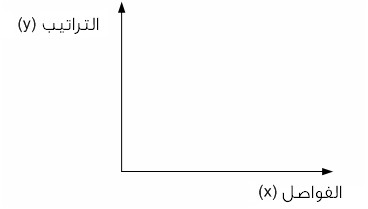
\includegraphics[width=0.4\textwidth]{Chapter_II-6_Axis}
\end{figure}

عندما نعمل في
\textenglish{2D}
لدينا محوران : محور الفواصل (من اليسار إلى اليمين) و محور التراتيب (من الأسفل إلى الأعلى). من العادة أن نرمز للفواصل بمتغيّر يدعى
\InlineCode{x}
و للتراتيب بـ\InlineCode{y}.

هل يمكنك كتابة هيكل
\InlineCode{Coordinates}
يسمح بتخزين كلّا من الفاصلة
(\InlineCode{x})
و الترتيبة
(\InlineCode{y})
لنقطة ما~؟\\
هيّا، هيّا، الأمر ليس صعبا :

\begin{Csource}
struct Coordinates
{
	int x; // Abscissas
	int y; // Ordinates
};
\end{Csource}

هيكلنا يسمّى
\InlineCode{Coordinates}
و هو متكوّن من متغيرين
\InlineCode{x}
و
\InlineCode{y}
أي الفاصلة
(\textenglish{Abscissa})
و الترتيبة
(\textenglish{Ordinate}).

إن أردنا، يمكننا بسهولة إنشاء هيكل
\InlineCode{Coordinates}
من أجل
\textenglish{3D} :
يكفي فقط إضافة متغيّر ثالث (مثلا
\InlineCode{z})
يدلّ على الارتفاع. بهذا سيكون لدينا هيكل لإدارة النقاط الثلاثيّة الأبعاد في الفضاء~!

\subsection{جدول داخل هيكل}

يمكن للهياكل أن تحتوي على جداول. هذا جيّد، إذ يمكننا أن نضع داخلها جداول
\InlineCode{char}،
(سلاسل محرفيّة) بدون أيّة مشاكل.\\
فلنتخيل هيكلاً
\InlineCode{Person}
و الذي يحتوي على معلومات عن شخص :

\begin{Csource}
struct Person
{
	char firstName[100];
	char lastName[100];
	char address[1000];
	int age;
	int boy; // Boolean : 1 = boy, 0 = girl
};
\end{Csource}

هذا الهيكل متشكّل من 5 متغيرات داخليّة، الثلاث الأولى هي سلاسل محرفيّة لتخزين الاسم، اللقب و العنوان.\\
المتغيران الأخيران يخزّنان عُمر و جنس الشخص. الجنس هو متغيّر منطقي، 1 = صحيح = ولد و 0 = خطأ = بنت.

يمكن لهذا الهيكل أن يساعدنا في كتابة برنامج مذكّرة عناوين. يمكنك بالطبع إضافة القدر الذين تريد من المتغيرات داخل الهيكل من أجل إتمامها إذا أردت. لا يوجد حدّ لعدد المتغيّرات في هيكل.

\section{استعمال هيكل}

و الآن، بما أن الهيكل معرّف في ملف
\InlineCode{.h}،
سنتمكّن من استعماله في دالة موجودة بملف
\InlineCode{.c}.\\
أنظر كيف نقوم بإنشاء متغير من نوع
\InlineCode{Coordinates}
(الهيكل الّذي عرّفناه سابقا) :
\begin{Csource}
#include "main.h" // Including the files that contains the prototypes and structures
int main(int argc, char *argv[])
{
	struct Coordinates point; // Creating a variable "point" of type Coordinates
	return 0;
}
\end{Csource}
هكذا نكون قد أنشأنا متغيراً
\InlineCode{point}
من نوع
\InlineCode{Coordinates} !
هذا المتغير سيحمل داخله مركّبين (متغيرين داخليين) :
\InlineCode{x}
و
\InlineCode{y}
(فاصلته و ترتيبته).

\begin{question}
  هل من اللازم أن نضع الكلمة المفتاحية
\InlineCode{struct}
عند تعريف المتغير ؟
\end{question}

نعم، فهذا يسمح للحاسوب بأن يفرّق بين نوع عادي (مثل
\InlineCode{int})
و نوع مخصّص.\\
المبرمجون وجدوا أنه من المتعب جدّا أن يكتبوا في كلّ مرة الكلمة
\InlineCode{struct}
في كلّ تعريف لمتغيّر مخصّص.
لمعالجة هذا المشكل، اخترعوا تعليمة خاصّة : الـ\InlineCode{typedef}.

\subsection{الـ\texttt{typedef}}

لنعد إلى الملف
\InlineCode{.h}
الذي يحمل تعريف هيكلنا من نوع
\InlineCode{Coordinates}.
سنضيف تعليمة اسمها
\InlineCode{typedef}
و الّتي تفيد في إعطاء اسم مستعار
(\textenglish{alias})
لهيكل، أي كتابة شيء مكافئ لكتابة آخر.

إذا، سنضيف سطرا يبدأ بـ\InlineCode{typedef}
قبل تعريف الهيكل مباشرة :

\begin{Csource}
typedef struct Coordinates Coordinates;
struct Coordinates
{
	int x;
	int y;
};
\end{Csource}

هذا السطر متكون من ثلاثة أجزاء :

\begin{itemize}
  \item \InlineCode{typedef} :
  تعني أننا سنقوم بإنشاء اسم مستعار لهيكل.
  \item \InlineCode{struct Coordinates} :
  هو اسم الهيكل الذي سنقوم بانشاء اسم مستعار له (أي "مكافئ").
  \item \InlineCode{Coordinates} :
  هو الاسم المكافئ.
\end{itemize}

ببساطة، هذا السطر يقول : "كتابة
\InlineCode{Coordinates}
مكافئ لكتابة
\InlineCode{struct Coordinates}".
بفعل هذا، لن يكون عليك كتابة الكلمة
\InlineCode{struct}
عند كلّ تعريف لمتغيّر من نوع
\InlineCode{Coordinates}.
يمكننا العودة إلى
\InlineCode{main}
و كتابة فقط :

\begin{Csource}
int main(int argc, char *argv[])
{
	 Coordinates point; // The computer understands that we are talking about "struct Coordinates" thanks to typedef
   return 0;
}
\end{Csource}

أنصحك أن تستعمل الـ\InlineCode{typedef}
مثلما فعلت أنا هنا من أجل
\InlineCode{Coordinates}.
أغلب المبرمجين يفعلون هذا. هذا يسمح لهم بعدم كتابة
\InlineCode{struct}
في كلّ مرّة. المبرمج الجيّد هو مبرمج كسول ! أي أنه يكتب أقل ما يمكن.

\subsection{تغيير مركّبات هيكل}

و الآن بعدما قمنا بإنشاء متغيّرنا
\InlineCode{point}،
نريد أن نغيّر إحداثيّاته.\\
كيف نصل إلى
\InlineCode{x}
و
\InlineCode{y}
الموجودة في المتغير
\InlineCode{point}
؟ هكذا :

\begin{Csource}
int main(int argc, char *argv[])
{
	Coordinates point;
	point.x = 10;
	point.y = 20;
	return 0;
}
\end{Csource}

بهذا نكون قد غيّرنا قيمة
\InlineCode{point}،
بإعطائه الفاصلة 10 و الترتيبة 20. نقطتنا أصبحت في الوضعية (10؛20) (هذا هو الترميز الرياضياتي للإحداثيّات).

لكي نتمكن من الوصول إلى مركّب في الهيكل، يجب كتابة :

\begin{Csource}
  variable.componentName
\end{Csource}

النقطة هي التي تفرّق بين المتغير و المركّب.

إن أخذنا الهيكل
\InlineCode{Person}
الذي رأيناه منذ قليل و نطلب الاسم و اللقب فسنفعل هكذا :

\begin{Csource}
int main(int argc, char *argv[])
{
	Person user;
	printf("What's your last name ? ");
	scanf("%s", user.lastName);
	printf("What's your first name ? ");
	scanf("%s", user.firstName);
	printf("You are %s %s", user.firstName, user.lastName);
	return 0;
}
\end{Csource}

\begin{Console}
What's your last name ? Dupont
What's your first name ? Jean
You are Jean Dupont
\end{Console}

نرسل المتغير
\InlineCode{user.lastName}
إلى الدالة
\InlineCode{scanf}،
و التي ستكتب مباشرة في
\InlineCode{user}.\\
نفعل نفس الشيء مع
\InlineCode{firstName}،
يمكننا فعل ذلك أيضا مع العنوان، العمر و الجنس، لكنّي لا أرغب بتكرار ذلك (يحب أن أكون مبرمجا !).

يمكن فعل هذا بدون معرفة الهياكل، فقط بإنشاء متغيّر
\InlineCode{lastName}
و آخر
\InlineCode{firstName}.\\
لكن الفائدة هنا هي أنه بهذه الطريقة يمكننا أن ننشئ متغيرا آخر من نوع
\InlineCode{Person}
و يكون لديه هو أيضا اسمه الخاص، لقبه الخاص، إلخ. يمكننا إذن فعل هذا :

\begin{Csource}
Person player1, player2;
\end{Csource}

و هكذا نخزّن معلومات كلّ لاعب. كلّ لاعب سيكون لديه اسمه الخاص، لقبه الخاص، إلخ.

يمكننا أن نفعل ما هو أفضل : يمكننا تعريف جدول من
\InlineCode{Person} !\\
القيام بهذا سهل :

\begin{Csource}
Person players[2];
\end{Csource}

و بعدها يمكننا الوصول إلى لقب اللاعب المتواجد بالخانة الأولى مثلا، هكذا :

\begin{Console}
players[0].lastName
\end{Console}

الفائدة من استعمال الجدول هنا، هو أنها بامكاننا استعمال حلقة لنقرأ المعلومات الخاصة باللاعب 1 و اللاعب 2 بدون الاضطرار إلى إعادة الشفرة مرّتين. يكفي تصفّح الجدول
\InlineCode{players}
و طلب كلّ مرّة اللقب، الاسم، العنوان \dots

\paragraph{تمرين :}
قم بتعريف جدول من نوع
\InlineCode{Person}،
و اقرأ المعلومات الخاصة بكلّ لاعب باستخدام حلقة. إبدأ بجدول ذي خانتين، و إن كان ذلك ممتعا، حاول تكبير العدد لاحقا.\\
في النهاية، عليك بإظهار المعلومات التي أخذتها من كلّ لاعب.

\subsection{تهيئة هيكل}

بالنسبة للهياكل، مثل كلّ المتغيرات، الجداول و المؤشّرات، فنحن نفضّل أن نعطيها قيما ابتدائية كي نضمن أنّها لن تحوي "قيما عشوائية". في الواقع، أعيد تذكيرك، المتغير الّذي يتمّ إنشائه يأخذ القيمة الموجودة في الذاكرة حيث تمّ وضعه. أحيانا تكون هذه القيمة $ 0 $، و أحيانا بقايا برنامج مرّ قبلك، لذلك ستكون قيمته شيئا لا معنى له، مثل
$-84570$.

للتذكير، هكذا نقوم بالتهيئة :

\begin{itemize}
  \item  المتغير : نعطيه القيمة 0 (الحالة الأبسط).
  \item المؤشّر : نجعل قيمته
\InlineCode{NULL}.
بالمناسبة فـ\InlineCode{NULL}
هي
\InlineCode{\#define}
موجود في مكتبة
\InlineCode{stdlib.h}
و هي عادة 0، لكنّنا نستمرّ في استخدام
\InlineCode{NULL}
للمؤشرات لكي نبيّن أنّها مؤشّرات و ليست متغيّرات عاديّة.
  \item الجدول : نضع كلّ خاناته على القيمة 0.
\end{itemize}

بالنسبة للهياكل، فالتهيئة شبيهة بتلك الخاصّة بالجدول. في الواقع، يمكننا القيام بها عند التصريح عن المتغيّر :

\begin{Csource}
Coordinates point = {0, 0};
\end{Csource}

و هذا يعرّف بالترتيب :
\InlineCode{point.x = 0}
و
\InlineCode{point.y = 0}.
لنعد إلى الهيكل
\InlineCode{Person}
(الذي يحتوي سلاسل محرفيّة). يمكننا أن نعطي قيمة ابتدائية للسلاسل بكتابة فقط
\InlineCode{""}
(لا شيء ببن علامتي الاقتباس). لم أعلمك هذا الشيء في الفصل الخاصّ بالسلاسل، لكنّ الوقت ليس متأخّرا على تعلّمها.
يمكننا إذن تهيئة على الترتيب
\InlineCode{firstName}،
\InlineCode{lastName}،
\InlineCode{address}،
\InlineCode{age}،
و
\InlineCode{boy}
هكذا :

\begin{Csource}
Person user= {"", "", "", 0, 0};
\end{Csource}

رغم ذلك، أنا لا أستخدم هذه التقنيّة كثيرا. أفضّل أن أرسل متغيّري، مثلا
\InlineCode{point}،
إلى دالّة
\InlineCode{initializeCoordinates}
تقوم بالتهيئات من أجلي على متغيري.\\
لفعل هذا، يجب إرسال مؤشّر نحو متغيري. في الواقع، إن أرسلت فقط المتغيّر، سيتم إنشاء نسخة عنه (مثل أيّ متغيّر عادي) و تعديل قيم النسخة لا قيم المتغيّر. راجع الخيط الأحمر من فصل المؤشرات إن نسيت كيف يعمل هذا الأمر.

يجب إذن تعلّم كيفيّة استخدام المؤشرات على الهياكل. الأمور بدأت تصعب قليلا !

\section{مؤشّر نحو هيكل}

المؤشّر على الهيكل يتمّ إنشائه بنفس طريقة إنشاء مؤشّر على
\InlineCode{int}
أو
\InlineCode{double}
أو أيّ نوع قاعديّ آخر :

\begin{Csource}
Coordinates* point = NULL;
\end{Csource}
بهذا نكون قد عرّفنا مؤشّرا نحو
\InlineCode{Coordinates}
اسمه
\InlineCode{point}.\\
و لأن التذكير لن يضرّ أحدا، أعيد إخبارك بأنه من الممكن وضع النجمة أمام اسم المتغيّر، فهذه الكتابة مكافئة تماما للسابقة~:

\begin{Csource}
Coordinates *point = NULL;
\end{Csource}

أنا أفعل هكذا كثيرا، لأنه لتعريف عدّة مؤشرات على سطر واحد، سيكون علينا وضع النجمة أمام اسم كل واحد منها :

\begin{Csource}
Coordinates *point1 = NULL, *point2 = NULL;
\end{Csource}

\subsection{إرسال هيكل إلى دالة}

الشيء الذي يهمّنا هنا، هو كيفيّة إرسال مؤشر هيكل إلى دالة كي تقوم هذه الأخيرة بتعديل محتواه.

هذا ما سنقوم به في هذا المثال، سنقوم بإنشاء متغير من نوع
\InlineCode{Coordinates}
في
\InlineCode{main}،
و نرسل عنوانه إلى
\InlineCode{initializeCoordinates}.
دور هذه الدالة هو إعطاء القيمة 0 لعناصر الهيكل.

دالتنا
\InlineCode{initializeCoordinates}
ستأخذ معاملا واحدا : مؤشر نحو هيكل من نوع
\InlineCode{Coordinates}
(أي
\InlineCode{*Coordinates}).

\begin{Csource}
int main(int argc, char *argv[])
{
	Coordinates myPoint;
	initializeCoordinates(&myPoint);
	 return 0;
}
void initializeCoordinates(Coordinates* point)
{
	// Initializing each member of the structure here
}
\end{Csource}

متغيري
\InlineCode{myPoint}
تم إنشاؤه في
\InlineCode{main}.\\
نقوم يارسال عنوانه إلى الدالة
\InlineCode{initializeCoordinates}
الّتي تسترجعه على شكل متغيّر يسمّى
\InlineCode{point}
(كان بإمكاننا تسميته كما شئنا، هذا الأمر ليس له أيّ تأثير).

الآن بما أنّنا داخل الدالة
\InlineCode{initializeCoordinates}،
سنقوم يتهيئة قيم المتغير
\InlineCode{point}
واحدة بواحدة.\\
يجب عدم نسيان وضع النجمة أمام اسم المؤشر للوصول إلى المتغير. إن لم تفعل، فأنت تخاطر بتغيير العنوان، و ليس هذا ما نريد فعله.

و لكن هاهي مشكلة \dots لا يمكننا القيام مباشرة بهذا :

\begin{Csource}
void initializeCoordinates(Coordinates* point)
{
	*point.x = 0;
	*point.y = 0;
}
\end{Csource}

سيكون ذلك سهلا جدّا \dots لماذا لا يمكننا القيام بهذا ؟
لأنّ النقطة تطبّق على
\InlineCode{point}
فقط و ليس على
\InlineCode{*point}.
لكنّ ما نريده هو الوصول إلى
\InlineCode{*point}
لتغيير قيمته.\\
لحلّ هذا المشكل، يجب وضع الأقواس حول
\InlineCode{*point}،
هكذا ستطبّق النقطة على
\InlineCode{*point}
و ليس فقط على
\InlineCode{point} :

\begin{Csource}
void initializeCoordinates(Coordinates* point)
{
	(*point).x = 0;
	(*point).y = 0;
}
\end{Csource}

هذه الشفرة تعمل، يمكنك تجريبها. المتغير من نوع
\InlineCode{Coordinates}
تمّ إرساله إلى الدالة التي هيّأت
\InlineCode{x}
و
\InlineCode{y}
على 0.

\begin{information}
في لغة الـ\textenglish{C}،
نهيّئ عادة هياكلنا بالطريقة الّتي رأيناها سابقا. بالمقابل، في لغة الـ\textenglish{C++}،
التهيئة تكون في الغالب داخل "دوال".
إن لغة
\textenglish{C++}
ليست سوى "تحسين خارق" للهياكل. كثير من الأشياء تبدأ من هذا و أحتاج إلى كتاب كامل لأتحدّث عنها (كلّ شيء في وقته).
\end{information}

\subsection{اختصار عمليّ و مستعمل بكثرة}

سترى أننا سنستعمل كثيراً مؤشرات نحو هياكل. بصراحة، يجب أن أعترف لك بأنّه
في لغة الـ\textenglish{C}
نستخدم  المؤشرات نحو الهياكل أكثر من استعمال الهياكل وحدها. لهذا فعندما أقول لك بأنّ المؤشرات ستظلّ تتبعك حتّى إلى قبرك، فأنا لا أقولها تقريبا من أجل المزاح !

بما أن المؤشرات نحو الهياكل مستعملة بكثرة، نجد أنفسنا نستعمل هذه الكتابة كثيرا :
\begin{Csource}
(*point).x = 0;
\end{Csource}

مرّة أخرى، المبرمجون وجدوا هذه الكتابة طويلة جدّا. الأقواس حول
\InlineCode{*point}،
يا لها من بلوى~! إذن، بما أن المبرمجين أشخاص كسالى (لقد قلت هذا سابقا على ما أعتقد)، فقد اخترعوا هذا الاختصار :

\begin{Csource}
point->x = 0;
\end{Csource}

هذا الاختصار يتمّ كتابته بمطّة
\InlineCode{-}
متبوعة بعلامة ترتيب
\InlineCode{>}.

كتابة
\InlineCode{point->x}
هو إذن مكافئ
\underline{تماما}
لكتابة
\InlineCode{(*point).x}.

\begin{warning}
  لا تنس أننا لا نستطيع استعمال السهم إلا مع المؤشرات.\\
إن كنت تعمل على المتغير مباشرة، يجب عليك استخدام النقطة كما رأينا في البداية.
\end{warning}

لنعد إلى دالتنا
\InlineCode{initializeCoordinates}
يمكننا كتابتها بالشكل التالي :

\begin{Csource}
void initializingCoordinates(Coordinates* point)
{
	point->x = 0;
	point->y = 0;
}
\end{Csource}

و تذكّر جيّدا اختصار السهم، سنستعمله كثيراً من الآن. و خاصّة لا تخلط بين السهم و "النقطة". السهم مخصّص للمؤشّرات، "النقطة" مخصّصة للمتغيّرات. استخدم هذا المثال الصغير للتذكّر :

\begin{Csource}
int main(int argc, char *argv[])
{
	Coordinates  myPoint;
	Coordinates *pointer = &myPoint;
	myPoint.x = 10; // We work on a variable, we use the "dot"
	pointer->x = 10; // We work on a pointer, we use the arrow
	return 0;
}
\end{Csource}

نغيّر قيمة
\InlineCode{x}
إلى 10 بطريقتين مختلفتين، هنا : الطريقة الأولى هي بالعمل مباشرة على المتغير، و الطريقة الثانية باستعمال المؤشر.

\section{التعدادات}

التعدادات هي طريقة مختلفة قليلاً لنعرّف نوع متغيرات خاص بنا.

التعداد ليس متكوّنا من "مركّبات"  كما هو الحال مع الهياكل. و إنما هو مجموعة من "القيم الممكنة" لمتغيّر. التعداد سيأخذ إذن خانة واحدة في الذاكرة و هذه الخانة تأخذ قيمة واحدة من مجموع القيم التي قمت بتعريفها (واحدة فقط في كلّ مرّة).
هذا مثال عن تعداد :
\begin{Csource}
typedef enum Volume Volume;
enum Volume
{
	LOW, MEDIUM, HIGH
};
\end{Csource}
تلاحظ أننا نستعمل
\InlineCode{typedef}
هنا أيضا، مثلما رأينا لحد الآن.

لكي نقوم بتعريف تعداد نستعمل الكلمة المفتاحية
\InlineCode{enum}.
اسم التعداد هنا هو
\InlineCode{Volume}.
إنّه نوع مخصّص قمنا بتعريفه يمكن له أن يأخذ واحدة من الثلاث قيم الّتي وضعناها : إما
\InlineCode{LOW}
أو
\InlineCode{MEDIUM}
أو
\InlineCode{HIGH}.

يمكننا إذن أن نعرّف متغيرا اسمه
\InlineCode{music}
من نوع
\InlineCode{Volume}
لتخزين مستوى صوت الموسيقى.\\
يمكننا تهيئة الموسيقى على المستوى
\InlineCode{MEDIUM} :
\begin{Csource}
Volume music = MEDIUM;
\end{Csource}
يمكننا لاحقاً في الشفرة، أن نغيّر قيمة مستوى الصوت و وضعها إمّا على
\InlineCode{HIGH}
أو على
\InlineCode{LOW}.

\subsection{إرفاق قيم التعداد بأعداد}
قد لاحظت أنّي كتبت القيم الممكنة بأحرف كبيرة. هذا يفترض به أن يذكّرك بالثوابت و
\InlineCode{\#define}،
أليس كذلك ؟

في الواقع، إنّ هذا مشابه كثيرا و لكنّه ليس نفس الشيء.\\
المترجم يقوم تلقائيا بارفاق قيم التعداد بأعداد موافقة لها.


في حالة تعدادنا
\InlineCode{Volume}،
\InlineCode{LOW}
سيتم ارفاقها بالقيمة 0،
\InlineCode{MEDIUM}
بالقيمة 1،
و
\InlineCode{HIGH}
بالقيمة 2.\\
الإرفاق يتمّ تلقائيّا انطلاقا من 0.

خلافا لـ\InlineCode{\#define}،
فالمترجم هو من يرفق
\InlineCode{MEDIUM}
بـ1 مثلا، وليس المعالج القبلي. لكنّ هذا سيكون تقريبا مكافئا له.\\
بطبيعة الحال، عندما هيّئنا المتغيّر
\InlineCode{music}
على
\InlineCode{MEDIUM}،
فإنّنا قد وضعنا القيمة 1 في خانة الذاكرة الموافقة.

\begin{question}
عمليّا، هل يهمّنا أن نعرف أنّ
\InlineCode{MEDIUM}
تساوي 1،
\InlineCode{HIGH}
تساوي 2، إلخ. ؟
\end{question}

لا. فهذا حقيقة لا يعنينا. المترجم هو من سيقوم تلقائيّا بإرفاق العدد المناسب إلى كلّ قيمة. بفضل هذا، ليس عليك سوى كتابة :
\begin{Csource}
if (music == MEDIUM)
{
	// Play music with medium volume
}
\end{Csource}
لا يهمّ ما هي قيمة
\InlineCode{MEDIUM}،
ستترك المترجم يهتمّ بالأعداد.

الفائدة من كلّ  هذا ؟  هي أنها تجعل الشفرة قابلة للقراءة جيّدا. في الواقع، أيّ شخص يمكنه بسهولة قراءة
\InlineCode{if}
السابق (نفهم جيّدا أنّ الشرط يعني "إن كانت الموسيقى بمستوى صوت متوسّط").

\subsection{ارفاق قيمة محددة}
حاليّا، كان المترجم هو من يقرّر إرفاق العدد 0 ثم 1، 2، 3
 بالترتيب.\\
من الممكن طلب إرفاق قيمة محدّدة لكلّ عنصر من التعداد.

ما الفائدة التي يمكن تحصيلها من هذا ؟ حسنا فلنفرض أنّه في حاسوبك، الصوت يتم تحديده بقيمة بين 0 و 100 (0 = لا صوت، 100 = 100\%
من الصوت)، فسيكون من الجيد ارفاق قيمة محدّدة بكلّ عنصر :
\begin{Csource}
typedef enum Volume Volume;
enum Volume
{
	LOW = 10, MEDIUM = 50, HIGH = 100
};
\end{Csource}
هنا، المستوى
\InlineCode{LOW}
يوافق 10\%
من المستوى، المستوى
\InlineCode{MEDIUM}
يوافق 50\%،
إلخ.\\
يمكننا بسهولة إضافة بعض القيم الأخرى مثل
\InlineCode{MUTE}.
نرفق في هذه الحالة
\InlineCode{MUTE}
بالقيمة \dots 0 ! لقد فهمت.

\section*{ملخّص}

\begin{itemize}
  \item الهيكل هو نوع بيانات مخصّص يمكنك إنشاؤه و استخدامه في برامجك. يجب عليك تعريفه، عكس الأنواع القاعديّة مثل
\InlineCode{int}
و
\InlineCode{double}
الّتي نجدها في كلّ البرامج.
  \item الهيكل يتكوّن من "متغيّرات داخليّة" تكون عادة من أنواع قاعديّة مثل
\InlineCode{int}
و
\InlineCode{double}،
و أيضا من الجداول.
  \item نستطيع الوصول إلى أحد مركّبات الهيكل بفصل اسم المتغيّر و المركّب بنقطة :
\InlineCode{player.firstName}.
  \item إذا كنّا نتعامل مع مؤشر نحو هيكل و أردنا الوصول إلى أحد مركّباته، نستخدم السهم بدل النقطة :\\
\InlineCode{playerPointer->firstName}.
  \item التعداد هو نوع مخصّص يمكنه فقط أخذ إحدى القيم المسبقة التعريف :
\InlineCode{LOW}،
\InlineCode{MEDIUM}
أو
\InlineCode{HIGH}
مثلا.
\end{itemize}

  \chapter{قراءة و كتابة الملفات}
المشكل مع استعمال المتغيّرات، هو أنها موجودة فقط في الذاكرة العشوائية
\textenglish{RAM}.
بخروجنا من البرنامج، كلّ المتغيّرات يتم حذفها من الذاكرة و لن يصبح ممكنا إستعادة قيمها. كيف يمكننا إذن أن نحتفظ بأحسن العلامات التي تحصّلنا عليها في لعبة ؟ كيف يمكننا إنشاء محرر نصوص إذا كان كلّ النصّ  المكتوب يختفي بمجرّد إيقاف البرنامج ؟

لحسن الحظّ يمكننا القراءة من الملفاّت و كذا الكتابة فيها في لغة
\textenglish{C}.
هذه الملفّات مُخزّنة في القرص الصلب
(\textenglish{Hard disk})
الخاص بالحاسوب : الشيء الإيجابيّ إذن هو أنها تبقى محفوظة، حتّى عند إيقاف البرنامج أو الحاسوب.

للقراءة من الملفات و الكتابة فيها، سنحتاج إلى استعمال كلّ ما درسناه حتّى الآن : المؤشرات، الهياكل، السلاسل المحرفيّة، الخ.

\section{فتح و غلق ملف}
للقراءة و الكتابة في الملفّات، سنستعمل دوالاً معرّفة في المكتبة
\InlineCode{stdio}
التي استعملناها سابقاً.\\
نعم، هذه المكتبة تحتوي على الدالتين
\InlineCode{scanf}
و
\InlineCode{printf}
اللتان نعرفهما جيّدا ! لكن ليس هذا فحسب : يوجد بها الكثير من الدوال الأخرى، خصوصا التي تعمل على الملفات.

\begin{information}
  كل المكتبات التي استعملناها حتّى الآن
(\InlineCode{stdlib.h}، \InlineCode{stdio.h}، \InlineCode{math.h}، \InlineCode{string.h}...)
تشكّل ما نسميه بالمكتبات القياسية
(\textenglish{standard libraries})،
و هي مكتبات تأتي تلقائيا مع البيئة التطويرية التي تستخدمها و لديها الميزة في أنّها تعمل على كل أنظمة التشغيل. بالإمكان استعمالها في أيّ مكان، سواء كنت في
\textenglish{Windows}،
أو
\textenglish{GNU/Linux}
أو
\textenglish{Mac}
أو غير ذلك.
المكتبات القياسيّة ليست كثيرة و لا تمكّننا من القيام بأكثر من بعض الأمور الأساسيّة، كما فعلنا لغاية الآن. للحصول على وظائف أكثر تقدّما، كفتح النوافذ، يجب تحميل و تثبيت مكتبات جديدة. سنرى ذلك قريبا !
\end{information}

تأكّد إذن، للبدأ، أن تقوم بتضمين المكتبتين
\InlineCode{stdio.h}
و
\InlineCode{stdlib.h}
على الأقل أعلى ملفكم
\InlineCode{.c} :

\begin{Csource}
#include <stdlib.h>
#include <stdio.h>
\end{Csource}

هاتان المكتبتان ضروريتان و أساسيّتان لدرجة أنّي أنصحك بتضمينهما في كلّ البرامج التي تكتبها في المستقبل، أيّا كانت.

حسناً و بعدما قمنا بتضمين المكتبتين، يمكننا أن ننطلق في بالأمور الجدّيّة. إليك الخطوات التي يجب إتّباعها دائماً حينما تريد العمل على ملف، سواء للقراءة منه أو للكتابة فيه :
\begin{itemize}
  \item نقوم بمناداة دالة
\textbf{فتح الملف}
\InlineCode{fopen}
التي تقوم بإرجاع مؤشّر نحو هذا الملف.
  \item \textbf{نتأكّد من نجاح عمليّة الفتح}
(أي إن كان الملفّ موجودا) باختبار قيمة المؤشر الذي أرجعته الدالة. فإن كان المؤشر يساوي
\InlineCode{NULL}،
فهذا يعني أنّ فتح الملف لم ينجح، في هذه الحالة لا يمكننا الإكمال (يجب أن نظهر رسالة خطا).
  \item إذا تم الفتح بنجاح (أي أن قيمة المؤشر تختلف عن
\InlineCode{NULL})،
سنستمتع
\textbf{بالكتابة على الملف أو القراءة منه}،
و ذلك باستخدام دوال سنراها لاحقاً.
  \item بمجرّد أن
\textbf{ننهي العمل على الملف}،
يجب تذكّر "غلقه" باستعمال الدالة
\InlineCode{fclose}.
\end{itemize}
سنتعلّم كخطوة أولى كيف نستخدم
\InlineCode{fopen}
و
\InlineCode{fclose}،
حينما تتعلّم هذا، سنتعلّم كيف نقرأ محتواه و نكتب نصّا فيه.

\subsection{\texttt{fopen} : فتح ملف}
في فصل السلاسل المحرفيّة، كنا نستعين بنماذج الدوال مثل "دليل استخدام". هذا ما يفعله المبرمجون غالبا : يقرؤون نموذج دالة و يفهمون كيف يستخدمونها. مع ذلك، أعلم أنّنا بحاجة إلى بعض الشروحات البسيطة !

لهذا فلنرى قليلاً نموذج
\InlineCode{fopen} :

\begin{Csource}
FILE* fopen(const char* fileName, const char* openMode);
\end{Csource}

هذه الدالة تنتظر معاملين :
\begin{itemize}
  \item اسم الملف الذي نريد فتحه.
  \item أسلوب فتح الملف، أي دلالة تذكر ما الّذي تريد فعله : القراءة من الملف، أو الكتابة فيه، أو كليهما.
\end{itemize}

هذه الدالة ترجع... مؤشّرا على
\InlineCode{FILE} !
إنّه مؤشّر على هيكل من نوع
\InlineCode{FILE}.
هذا الهيكل متواجد في المكتبة
\InlineCode{stdio.h}.
يمكنك فتح الملف لترى مما يتكوّن النوع
\InlineCode{FILE}،
لكن هذا ليس ما يهمّنا.

\begin{question}
  لكن لِمَ اسم الهيكل كله بأحرف كبيرة؟ اعتقدت أن الأسماء بالأحرف الكبيرة حجزناها للثوابت و لـ\InlineCode{\#define} ؟
\end{question}

هذه "القاعدة"، أنا من قمت بتحديدها (و كثير من المبرمجين يتيعونها)، و لكنّها لم تكن أبدا مفروضة. و يبدو أنّ من برمجوا
\InlineCode{stdio.h}
لا يتبعون نفس القواعد !\\
هذا لا يجب أن يشوّشك كثيرا. سوف ترى أنّ المكتبات الّتي سندرسها لاحقا تتبّع نفس القواعد التي أتّبعها، أي أن اسم الهيكل يبتدئ فقط بحرف واحد كبير.

لنعد إلى دالتنا
\InlineCode{fopen}،
إنها تقوم بارجاع
\InlineCode{FILE*}.
إنه من المهم جدّا استرجاع هذا المؤشّر كي نتمكّن لاحقاً من القراءة و الكتابة في الملف.  و لهذا سنقوم بإنشاء مؤشّر على
\InlineCode{FILE}،
في بداية دالتنا
(\InlineCode{main}
مثلا) :

\begin{Csource}
int main(int argc, char *argv[])
{
	FILE* file = NULL;
	return 0;
}
\end{Csource}

لقد هيّأنا المؤشّر على
\InlineCode{NULL}
من البداية. أذكّرك بأنّ هذه قاعدة أساسيّة أن تهيّأ كلّ المؤشّرات على
\InlineCode{NULL}
إنّ لم تكن لديك قيمة أخرى لإعطائها. إن لم تفعل ذلك، فأنت تزيد كثيرا خطر وجود أخطاء لاحقا.

\begin{information}
  إنه ليس ضرورياً أن تكتب
\InlineCode{struct FILE* file = NULL}،
لأن منشئي
\InlineCode{stdio.h}
قد وضعوا
\InlineCode{typedef}
كما علّمتك منذ مدّة قصيرة.
لاحظ أن شكل الهيكل قد يتغيّر من نظام تشغيل إلى آخر (لا تملك بالضرورة نفس المركّبات في كل الأنظمة). لهذا فلن نعدّل محتوى
\InlineCode{FILE}
مباشرة (لا نقوم بـ\InlineCode{file.element}
مثلا). بل سنكتفي باستدعاء دوال، تتعامل مع
\InlineCode{FILE}
نيابة عناً.
\end{information}

الآن سنقوم بمناداة الدالة
\InlineCode{fopen}،
و استرجاع القيمة الّتي تعيدها في المؤشر
\InlineCode{file}.
و لكن قبل هذا يجب أن اشرح لك كيف تستخدم المعامل الثاني
\InlineCode{openMode}.
في الواقع، هناك شفرة تدلّ للحاسوب على أنك تريد أن تفتح الملف بوضع القراءة فقط، الكتابة فقط أو الاثنين معاً.\\
هذه هي أوضاع فتح الملف المختلفة :
\begin{itemize}
  \item \textbf{\textenglish{"r"} :
قراءة فقط
(\textenglish{read only})}.
يمكنك قراءة محتوى الملف، و لكن لا يمكنك الكتابة فيه.
\textit{يجب أن يكون الملف موجوداً من قبل}.
  \item \textbf{\textenglish{"w"} :
كتابة فقط
(\textenglish{write only})}.
يمكنك الكتابة في الملف، لكن لا يمكنك قراءة محتواه.
\textit{إذا لم يكن الملف موجوداً من قبل، فإنه سيتم إنشاؤه}.
  \item \textbf{\textenglish{"a"} :
إلحاق
(\textenglish{append})}.
يمكنك الكتابة في الملف، إنطلاقا من نهايته.
\textit{إن لم يكن الملف موجوداً، فسيتم إنشاؤه}.
  \item \textbf{\textenglish{"r+"} :
قراءة و كتابة
(\textenglish{read and write})}.
يمكنك القراءة من الملف و الكتابة فيه.
\textit{يجب أن يكون الملف موجوداً من قبل}.
  \item \textbf{\textenglish{"w+"} :
قراءة و كتابة مع مسح المحتوى أوّلا}.
سيتم تفريغ الملف من محتواه أولاً، ثم بإمكانك الكتابة فيه و قراءة محتواه بعد ذلك.
\textit{إن لم يكن الملف موجوداً من قبل، سيتم إنشاؤه}.
  \item \textbf{\textenglish{"a+"}
إلحاق مع القراءة / الكتابة في آخر الملف}.
يمكنك القراءة و الكتابة إنطلاقا من نهاية الملف.
\textit{إن لم يكن موجوداً، سيتم إنشاؤه}.
\end{itemize}

لمعلوماتك، أنا عرضت لك بعضا من أوضاع فتح ملف. في الحقيقة، يوجد ضعفها !
من أجل كل وضع رأيناه هنا، إن أضفت
\InlineCode{"b"}
بعد المحرف الأول
(\InlineCode{"rb"}، \InlineCode{"wb"}، \InlineCode{"ab"}، \InlineCode{"rb+"}، \InlineCode{"wb+"}، \InlineCode{"ab+"})،
فإن الملف سيتم فتحه بالوضع الثنائي
(\textenglish{binary}).
هذا وضع خاص قليلاً فلن ندرسه هنا. في الواقع وضع النص يختصّ بتخزين... النص، تماما كما يوحي الاسم (فقط المحارف القابلة للعرض). أما الوضع الثنائي، يسمح بتخزين المعلومات
بايتا بايتا
(\textenglish{Byte by byte})
(أرقام بشكل أساسي). هذا مختلف كثيرا. على أي حال فطريقة العمل هي تقريبا نفس الّتي سنراها هنا.

شخصياً، أستعمل كثيراً الأوضاع :
\InlineCode{"r"}
(قراءة)،
\InlineCode{"w"}
(كتابة)،
\InlineCode{"r+"}
(قراءة و كتابة في آن واحد). وضع
\InlineCode{"w+"}
خطر قليلاً لأنه يقوم بمسح محتوى الملف مباشرة، بدون أن يطلب التأكيد قبل القيام بذلك. إن هذا الوضع ليس مفيداً إلا إذا أردنا أن نعيد تهيئة الملف أوّلا.
وضع الإلحاق
(\InlineCode{"a"})
يمكنه أن يفيد في بعض الحالات، إذا كنت تريد إضافة معلومات إلى نهاية الملف.

\begin{information}
  إن كنت تريد قراءة ملفّ، فمن المستحسن وضع
\InlineCode{"r"}.
بالطبع، الوضع
\InlineCode{"r+"}
يعمل أيضا، لكن بوضع
\InlineCode{"r"}
فأنت تضمن أنّ الملفّ لا يمكن تعديله، هذا نوع من الحماية.
\end{information}

إن كتبت دالةً
\InlineCode{loadLevel}
(لتحميل مستوى في لعبة مثلا)، الوضع
\InlineCode{"r"}
كافٍ، أما إن أردت أن كتابة دالةٍ
\InlineCode{saveLevel}
(لحفظ المستوى) فستستعمل الوضع
\InlineCode{"w"}.

الشفرة التالية ستفتح الملف
\InlineCode{test.txt}
في وضع
\InlineCode{"r+"}
(قراءة و كتابة) :

\begin{Csource}
int main(int argc, char *argv[])
{
	FILE* file = NULL;
	file = fopen("test.txt", "r+");
	return 0;
}
\end{Csource}

المؤشّر
\InlineCode{file}
يصبح إذن مؤشراً على الملف
\InlineCode{test.txt}.

\begin{question}
  أين يجب أن يكون الملف
\InlineCode{test.txt}
؟
\end{question}

يجب أن يكون في نفس المجلّد الذي يتواجد به الملف التنفيذي
(\InlineCode{.exe}).\\
من أجل متطلّبات هذا الفصل، أطلب منك أن تقوم بإنشاء ملف
\InlineCode{test.txt}
في نفس المساؤ الذي به
\InlineCode{.exe}،
مثلما أفعل أنا (الشكل الموالي).

\Picture{Chapter_II-7_Files}

كما ترى فأنا أستعمل  حاليّا بيئة التطوير
\textenglish{Code::Blocks}
الأمر الذي يفسّر وجود ملف المشروع بصيغة
\InlineCode{.cbp}
(في مكان الصيغة
\InlineCode{.sln}
إن كنت تستعمل
\InlineCode{Visual C++}
مثلاً). باختصار، الأمر المهم هو أن برنامجي
(\InlineCode{tests.exe})
موجود في نفس مجلّد الملف الذي نريد قرائته أو كتابته
(\InlineCode{test.txt}).

\begin{question}
  هل يجب أن يكون الملف بصيغة
\InlineCode{.txt} ؟
\end{question}

لا، الأمر يعود إليك في اختيار صيغة الملف عندما تفتحه. أي أنه بإمكانك أن تخترع صيغتك الخاصّة
\InlineCode{.level}
لحفظ مستويات ألعابك مثلاً.

\begin{question}
  هل من الواجب أن يكون الملف الذي نريد فتحه في نفس دليل الملف التنفيذي ؟
\end{question}

لا أيضا. يمكنه أن يكون داخل مجلّد بذات الدليل :

\begin{Csource}
  file = fopen("directory/test.txt", "r+");
\end{Csource}

هنا، الملف
\InlineCode{test.txt}
في مجلّد  داخليّ اسمه
\InlineCode{directory}.
هذه الطريقة التي نسميها
\textit{المسار النسبي}
عمليّة أكثر. هكذا، يمكن للبرنامج أن يعمل أينما كان مثبّتا.

من الممكن أيضا فتح ملفّ أينما كان في القرص الصلب. في هذه الحالة يجب كتابة المسار الكامل (ما نسميه
\textit{المسار المطلق}) :

\begin{Csource}
  file = fopen("C:\\Program Files\\Notepad++\\readme.txt", "r+");
\end{Csource}

هذه الشفرة تفتح الملف
\InlineCode{readme.txt}
الموجود بـ\InlineCode{C:\textbackslash Program Files\textbackslash Notepad++}.

\begin{warning}
  تعمّدت استعمال شرطتبن خلفيّتين
\InlineCode{\textbackslash}
  كما تلاحظ. في الواقع، إن كتبت اشارة واحدة، سيعتقد الحاسوب أنني أريد أن استخدم رمزا خاصا (مثل الـ\InlineCode{\textbackslash n}
أو الـ\InlineCode{\textbackslash t}).
لكتابة شرطة خلفيّة في سلسلة، يجب كتابتها إذن مرّتين ! هكذا يمكن أن يفهم أنّك تريد استخدام الرمز
\InlineCode{\textbackslash}.
\end{warning}

المشكل مع المسارات المطلقة، هو أنها لا تعمل إلا مع نظام معيّن، فهي ليست حلّا محمولا إذن. أي أنه لو كنت تعمل على
\textenglish{GNU/Linux}
لكان عليك كتابة مسار كهذا مثلا :

\begin{Csource}
  file = fopen("/home/mateo/directory/readme.txt", "r+");
\end{Csource}

لهذا فأنا أنصحك بكتابة مسارات نسبية. لا تستعمل المسارات المطلقة إلا في حالة كان البرنامج مخصص لنظام تشغيل معيّن، ليعدّل على ملف معيّن في القرص الصلب.

\subsection{اختبار فتح ملف}
المؤشّر
\InlineCode{file}
يجب أن يحوي عنوان الهيكل من نوع
\InlineCode{FILE}،
و الذي نستعمله كواصف
(\textenglish{descriptor})
للملف. هذا الواصف تم تحميله من أجلك في الذاكرة من طرف الدالة
\InlineCode{fopen}.
بعد هذا، هناك احتمالان :

\begin{itemize}
  \item إمّا أن تنجح عملية الفتح، فسنتمكن من المواصلة (أي البدء في القراءة و الكتابة في الملف).
  \item إمّا ألّا تنجح لأن الملف ليس موجوداً أو أنه مستخدم من طرف برنامج آخر. في هذه الحالة، سنتوقف عن العمل على الملف.
\end{itemize}

مباشرة بعد فتح الملف، يجب التأكد ما إن تمت العملية بنجاح، أم لا. هذا أمر بسيط : إذا كانت قيمة المؤشر تساوي
\InlineCode{NULL}،
فإن الفتح قد فشل. إن كانت قيمته تساوي شيئا غير
\InlineCode{NULL}،
فقد تم الفتح بنجاح.\\
سنتبع إذن هذا المخطط التالي :

\begin{Csource}
int main(int argc, char *argv[])
{
	FILE* file = NULL;
	file = fopen("test.txt", "r+");
	if (file != NULL)
	{
    		// We can read or write in the file
	}
	else
	{
    		// We display an error message if we want
    		printf("Can't open the file test.txt");
	}
	return 0;
}
\end{Csource}

إفعل هذا دائما عند فتح أي ملف. إن لم تفعل و الملف غير موجود، فأنت تخاطر بتوقّف البرنامج بعدها.

  \chapter{الحجز الحيّ للذاكرة
(\textenglish{Dynamic memory allocation})}

كل المتغيّرات التي أنشأناها لحد الآن تمّ إنشاؤها تلقائيّا من طرف المترجم الخاصّ بلغة
\textenglish{C}.
لقد كانت الطريقة البسيطة. رغم ذلك، توجد طريقة يدوية أكثر لإنشاء متغيّرات و نسمّيها بالحجز الحيّ
(\textenglish{Dynamic allocation}).

من بين فوائد الحجز الحيّ هو السماح لبرنامج بحجز مكان لازم لتخزين جدول في الذاكرة لا يُعرف حجمه قبل بداية الترجمة. في الواقع، حتّى الآن، كان حجم جداولنا ثابتاً في الشفرة المصدريّة. بعد قراءة هذا الفصل، ستستطيع إنشاء جداول بطريقة أكثر مرونة !

من الضروري أن تتقن التعامل مع المؤشرات لتتمكّن من قراءة هذا الفصل ! إن كانت لديك بعض الشكوك حول المؤشرات، أنصحك بالذهاب لإعادة قراءة الفصل الموافق قبل البدأ.

عندما نقوم بالتصريح عن متغيّر، فإننا نقول أننا
\textbf{طلبنا حجز مكان في الذاكرة} :

\begin{Csource}
int myNumber = 0;
\end{Csource}

عندما يصل المترجم إلى سطر مشابه للسطر السابق، يقوم بالأمور التالية :
\begin{itemize}
  \item يقوم البرنامج بطلب إذن من نظام التشغيل
(\textenglish{Windows}، \textenglish{GNU/Linux}، \textenglish{Mac OS}...)
ليحجز شيئا من الذاكرة.
  \item يستجيب نظام التشغيل بإعطاء البرنامج عنوان الخانة حيث يمكنه تخزين المتغيّر (يعطيه العنوان الّذي حجزه له).
  \item عندما تنتهي الدالّة، المتغيّر يتم حذفه من الذاكرة. برنامجك يقول لنظام التشغيل : "أنا لم أعد بحاجة إلى المكان في الذاكرة الّذي حجزته في ذلك العنوان، شكرا ! التاريخ لا يحدّد إن كان البرنامج قد قال فعلا "شكرا" لنظام التشغيل، لكنّ هذا في مصلحته لأنّ نظام التشغيل هو الّذي يتحكم في الذاكرة !
\end{itemize}

لحد الآن كل الأمور كانت تلقائيّة. عندما نصرّح عن متغير فإن نظام التشغيل يتمّ استدعاءه تلقائياً من طرف البرنامج.
ما رأيك إذا بفعل هذا بطريقة يدوية ؟ ليس لأننا نريد أن نستمتع بفعل شيء معقّد، بل لأننا أحيانا نظطرّ لفعل ذلك !

في هذا الفصل سنقوم بـ :
\begin{itemize}
  \item دراسة كيف تعمل الذاكرة (نعم، مرّة أخرى !) لنعرف ما الحجم الذي يحجزه كل متغيّر حسب نوعه.
  \item ثمّ ندخل في موضوعنا الأساسي : سنرى كيف نطلب من نظام التشغيل يدويّا أن يحجز لنا مكانا في الذاكرة. هذا ما سنسميه الحجز الحيّ للذاكرة.
  \item و أخيراً، سنكتشف الفائدة من القيام بالحجز الحيّ بتعلّم إنشاء جدول ذو حجم غير معروف إلّا عند اشتغال البرنامج.
\end{itemize}

\section{حجم المتغيرات}
بحسب نوع المتغير التي نريد إنشاءه
(\InlineCode{int}،
\InlineCode{char}،
\InlineCode{float}...)
فنحن نحتاج إلى حجم معيّن من الذاكرة.

في الواقع، لتخزين عدد من
$-128$
إلى
$127$
(\InlineCode{char})
لن نحتاج إلا إلى بايت واحد من الذاكرة. هذا حجم صغير للغاية.\\
بالمقابل،
\InlineCode{int}
يحجز عادة حوالي 4 بايتات من الذاكرة. بينما
\InlineCode{double}
يحجز 8 بايتات.

المشكل هو ... أن هذا ليس دائما صحيحا. هذا يعتمد على الأجهزة : فقد يكون
\InlineCode{int}
يحجز 8 بايتات. من يعلم ؟\\
هدفنا هنا أن نتعرّف كم يحجز كلّ نوع من حجم في الذاكرة على حاسوبك.

توجد وسيلة سهلة جدّا لمعرفة هذا : استعمال العامل
\InlineCode{sizeof()}.\\
على عكس الظاهر، فهو ليس دالة، بل عبارة عن إحدى الوظائف الأساسية من لغة الـ\textenglish{C}،
يجب عليك فقط أن تضع بين القوسين النوع الذي تريد تحليله.\\
لمعرفة حجم
\InlineCode{int}،
يجب كتابة التالي :

\begin{Csource}
sizeof(int)
\end{Csource}

عند الترجمة، سيتم استبدال هذه الشفرة بعدد : عدد البايتات الّتي يحجزها
\InlineCode{int}
في الذاكرة. بالنسبة لي،
\InlineCode{sizeof(int)}
تساوي 4، و هذا يعني أنّ
\InlineCode{int}
يأخذ 4 بايتات. بالنسبة لك، ستكون نفس القيمة على الأرجح، لكنّها ليست قاعدة. جرّب لترى، بعرض القيمة عن طريق
\InlineCode{printf}
مثلا :

\begin{Csource}
printf("char : %d bytes\n", sizeof(char));
printf("int : %d bytes\n", sizeof(int));
printf("long : %d bytes\n", sizeof(long));
printf("double : %d bytes\n", sizeof(double))
\end{Csource}

بالنسبة لي ، هذا يظهر على الشاشة :

\begin{Csource}
char : 1 bytes
int : 4 bytes
long : 4 bytes
double : 8 bytes
\end{Csource}

لم أختبر كل الأنواع الّتي نعرفها، أتركك لتجرّب أحجام الأنواع الأخرى.

أنت تلاحظ أن
\InlineCode{int}
و
\InlineCode{long}
يحجزان نفس الحجم من الذاكرة. إنشاء
\InlineCode{long}
يعود تماما إلى إنشاء
\InlineCode{int}،
هذا يأخذ 4 بايتات من الذاكرة.

\begin{information}
في الواقع، النوع
\InlineCode{long}
هو مكافئ لنوع نسميه
\InlineCode{long int}،
و الذي هو مكافئ لنوع...
\InlineCode{int}
نفسه. باختصار، فإن هذه أسماء كثيرة مختلفة لأجل أشياء ليست بالكبيرة، في النهاية ! امتلاك أنواع مختلفة كثيرة كان أمرا مهمّا  في الوقت الذي لمّ تكن الحواسيب تملك كثيرا من ذاكرة. كنا نبحث دائما لاستخدام الحدّ الأدنى من الذاكرة باستخدام النوع المناسب.\\
اليوم، هذا لم يعد مفيدا كثيرا لأنّ ذاكرة الحاسوب صارت كبيرة جدّا. بالمقابل، هذه الأنواع لا تزال مفيدة إذا كنت تنشئ برامج للأنظمة المضمّنة
(\textenglish{Embedded systems})
حيث الذاكرة المتوفّرة أقل. أظن مثلا في البرامج الموجّهة للهواتف المحمولة، الأليّات، إلخ.
\end{information}

\begin{question}
هل بإمكاننا أن نُظهر حجم نوع مخصّص قمنا نحن بإنشائه (هيكل) ؟
\end{question}

نعم !
\InlineCode{sizeof()}
تعمل مع الهياكل أيضا !

\begin{Csource}
typedef struct ِCoordinates ِCoordinates ;
struct ِCoordinates
{
	int x;
	int y;
};
int main(int argc, char *argv[])
{
	printf("ِCoordinates  : %d bytes\n", sizeof(ِCoordinates));
	return 0;
}
\end{Csource}

\begin{Console}
Coordinates : 8 bytes
\end{Console}

كلما احتوى الهيكل من مركّبات كلّما أخذ حجما أكثر من الذاكرة. الأمر منطقي تماما، أليس كذلك ؟

\subsection{طريقة أخرى للنظر إلى الذاكرة}
لحد الآن، كل المخططات التي قدّمتها لك عن الذاكرة لم تكن دقيقة. سنجعلها أخيرا دقيقة حقا و صحيحة بما أننا تعلّمنا الآن كم يأخذ كل نوع من حجم بالذاكرة.

إن صرّحنا عن متغير من نوع
\InlineCode{int} :

\begin{Csource}
int number = 18;
\end{Csource}

و
\InlineCode{sizeof(int)}
يعطينا 4 بايت على حاسوبنا، هذا يعني أن المتغير يحجز 4 بايت في الذاكرة !

لنفترض أن المتغير
\InlineCode{number}
محجوز بالعنوان
$1600$
من الذاكرة. سيكون لدينا إذا المخطط التالي للذاكرة :

\Picture{Chapter_II-8_RAM-Schema-int}

هنا، يمكننا فعلاً أن نرى بأن المتغير
\InlineCode{number}
من النوع
\InlineCode{int}
يحجز 4 بايت من الذاكرة.
فهو يبدأ من العنوان
$1600$
و ينتهي عند العنوان
$1603$،
المتغير القادم لن يتم تخزينه إلا إبتداءً من العنوان
$1604$ !

إن جربنا نفس الشيء مع
\InlineCode{char}،
فالمتغير لن يأخذ سوى بايت واحد في الذاكرة (الشكل التالي) :

\Picture{Chapter_II-8_RAM-Schema-char}

تخيّل الآن جدولا من
\InlineCode{int} !\\
كل "خانة" من الجدول ستحجز 4 بايت. إن كان الجدول يحوي مثلاً  100 خانة :

\begin{Csource}
int table[100];
\end{Csource}

سنحجز إذن
$100 * 4 = 400$
بايت في الذاكرة.

\begin{question}
ماذا لو كان الجدول فارغاً، هل سيحجز 400 بايت ؟
\end{question}

نعم بالطبع ! فالمكان  في الذاكرة قد تمّ حجزه، و لا يملك أي برنامج الحقّ في استخدام هذه الخانات (غير هذا البرنامج). بمجرّد التصريح عن متغيّر، سيأخذ مكانه مباشرة المكان في الذاكرة.

لاحظ لو أننا ننشئ جدولا من نوع
\InlineCode{Coordinates} :

\begin{Csource}
Coordinates table[100];
\end{Csource}

سيستخدم هذه المرّة
$8 * 100 = 800$
بايت.

من المهمّ الفهم الجيّد لهذه الحسابات البسيطة لنواصل بقيّة الفصل.

\section{الحجز الحيّ للذاكرة}
فلندخل إلى صلب الموضوع. سأذكّرك بهدفنا : تعلّم كيفيّة طلب الذاكرة يدوياً.

سنحتاج إلى تضمين المكتبة
\InlineCode{stdlib.h}.
إن كنت قد اتّبعت نصائحي، فقد ضمّنتها في كلّ برامجك. هذه المكتبة تحتوي على دالّتين سنحتاج إليهما :
\begin{itemize}
  \item \InlineCode{malloc} ("\textenglish{Memory ALLOcation}"
بمعنى "حجز الذاكرة") : تطلب الإذن من نظام التشغيل لاستخدام الذاكرة.
  \item \InlineCode{free}
(تحرير) : تسمح للإشارة لنظام التشغيل بأننا لم نعد بحاجة إلى الذاكرة الّتي طلبناها. المكان في الذاكرة تمّ تحريره، يستطيع برنامج آخر الآن استخدامها عند الحاجة.
\end{itemize}

عندما تقوم بحجز يدوي للذاكرة، فعليك اتباع الخطوات التالية :
\begin{enumerate}
  \item استدعاء
\InlineCode{malloc}
من أجل طلب الذاكرة.
  \item اختبار القيمة التي تم ارجاعها من طرف
\InlineCode{malloc}
لمعرفة ما إن نجح نظام التشغيل في حجز الذاكرة.
  \item ما إن ننتهي من استخدام الذاكرة، يجب علينا تحريرها باستعمال
\InlineCode{free}.
إن لم نفعل هذا، فسنتعرّض لتسريبات ذاكرة، أي أنّ البرنامج يخاطر بحجز كثير من الذاكرة مع أنّه ليس بحاجة إلى كلّ هذا المكان.
\end{enumerate}

هل تذكّرك هذه الخطوات الثلاث بفصل الملفات ؟ نعم يجب أن تفعل ! المبدأ واحد تماما : نحجز، نختبر إن نجح الحجز، ثمّ نحرر عندما ننتهي من الاستعمال.

\subsection{\texttt{malloc}
لنطلب الإذن لحجز الذاكرة}
نموذج الدالة
\InlineCode{malloc}
هزليّ جدّا، سترى :

\begin{Csource}
void* malloc(size_t numberOfNecessaryBytes);
\end{Csource}

الدالة تأخذ معاملا واحدا : عدد البايتات الّتي يجب حجزها. هكذا، يكفي أن كتابة
\InlineCode{sizeof(int)}
لحجز مكان من أجل تخزين
\InlineCode{int}.

و لكنّ الشيء الذي يثير الفضول، هو القيمة التي ترجعها الدالة : إنّها تعيد ...
\InlineCode{void*} !
إذا لازلت تتذكّر فصل الدوال، كنت قد قلت لك بأن الكلمة
\InlineCode{void}
تعني "الفراغ" و نستعملها لنشير إلى أن الدالة لا تُعيد أية قيمة.

إذن هنا، لدينا دالة تُعيد ... "مؤشّراً نحو فراغ" ؟ هذه نكتة جيدة !\\
يبدو أن هؤلاء المبرمجين لديهم حسّ فكاهي متطوّر.

كن متأكّدا، يوجد سبب. في الحقيقة، هذه الدالة تعيد عنوان الخانة التي حجزها نظام التشغيل من أجل متغيّرك. إن استطاع النظام إيجاد مكان لك في العنوان
$1600$،
فالدالة ستعيد مؤشّرا يحوي العنوان
$1600$.

المشكل هو أن الدالة
\InlineCode{malloc}
لا تعرف نوع المتغير التي نريد إنشاءه. في الواقع، أنت لا تعطيها سوى معامل واحد : عدد البايتات في الذاكرة الّتي تحتاجها. فإذا طلبت 4 بايت، فهذا يمكن أن يعني
\InlineCode{int}
أو ربما
\InlineCode{long}
مثلا !

بما أنّ
\InlineCode{malloc}
لا تعرف أيّ نوع يجب عليها أن تعيد، فهي تعيد النوع
\InlineCode{void*}.
سيكون مؤشّرا نحو
\textit{أيّ نوع كان}.
يمكننا أن نقول أنّه مؤشّر جامع.

لننتقل إلى التطبيق.\\
إذا كنت أريد الاستمتاع بإنشاء متغير من نوع
\InlineCode{int}
يدويّا في الذاكرة، يجب أن أشير للـ\InlineCode{malloc}
أنني أحتاج إلى
\InlineCode{sizeof(int)}
بايت في الذاكرة.\\
أسترجع قيمة
\InlineCode{malloc}
في مؤشر على
\InlineCode{int} :

\begin{Csource}
int* allocatedMemory = NULL; // Create a pointer on int
allocatedMemory = malloc(sizeof(int)); // The function malloc puts the allocated address in the pointer.
\end{Csource}

في نهاية هذه الشفرة،
\InlineCode{allocatedMemory}
هو مؤشّر يحتوي على عنوان حجزه نظام التشغيل لك، لنقل مثلا القيمة
$1600$
للاكمال من مخططاتي السابقة.

\subsubsection{اختبار المؤشّر}
الدالة
\InlineCode{malloc}
أعادت في المتغير
\InlineCode{allocatedMemory}
عنوان الخانة التي تم حجزها بالذاكرة. هناك احتمالان :
\begin{itemize}
  \item إذا نجح الحجز، فالمؤشّر سيحتوي عنوانا.
  \item إذا فشل الحجز، فالمؤشّر سيحتوي العنوان
\InlineCode{NULL}.
\end{itemize}

إنه من النادر أن تفشل عملية حجز الذاكرة، لكن هذا ممكن. تخيّل أنك تطلب حجز 34
\textenglish{Go}
من الذاكرة العشوائية، في هذه الحالة، ستفشل عملية الحجز على أغلب الظن.

من المستحسن دائماً أن نختبر ما إن تمت العملية بنجاح. سنفعل هذا : إن فشل الحجز، فهذا يعني أن المساحة الحرّة من الذاكرة العشوائية لم تكن كافية (هذه حالة حرجة). في حالة كهذه، يجب إيقاف البرنامج فورا لأنّه، على أية حال، لن يكون قادراً على الاستمرار بشكل عاديّ.

سنستعمل دالة قياسيّة لم يسبق لنا رؤيتها حتّى الآن :
\InlineCode{exit()}.
هذه الأخيرة توقف البرنامج فورا. إنّها تأخذ معاملا : القيمة الّتي يجب إعادتها من طرف البرنامج (هذا في الحقيقة يوافق الـ\InlineCode{return}
الخاص بالـ\InlineCode{main}).

\begin{Csource}
int main(int argc, char *argv[])
{
	int* allocatedMemory = NULL;
	allocatedMemory = malloc(sizeof(int));
	if (allocatedMemory == NULL) // If the allocation has failed
	{
    exit(0); // Stop the program
	}
	// Else, we can continue the program normally.
	return 0;
}
\end{Csource}

إذا كان المؤشر مختلفا عن
\InlineCode{NULL}،
يمكن للبرنامج أن يواصل العمل، و إلا فيجب إظهار رسالة خطأ أو حتّى إنهاء البرنامج لأنّه لن يتمكّن من الاستمرار بشكل صحيح إن لّم يكن هناك مكان في الذاكرة.

\subsection{\texttt{free} :
تحرير الذاكرة}
مثلما استعملنا الدالة
\InlineCode{fclose}
لنغلق ملفاً لم نعد في حاجة إليه، سنستعمل الدالة
\InlineCode{free}
من أجل تحرير الذاكرة التي لم نعد بحاجة إليها.

\begin{Csource}
void free(void* pointer);
\end{Csource}

الدالة
\InlineCode{free}
بحاجة فقط إلى عنوان الذاكرة المراد تحريرها. سنرسل لها إذن مؤشّرنا، أي
\InlineCode{allocatedMemory}
في مثالنا.\\
إليكم المخطط الكامل و النهائي، مشابه بشكل كبير لما رأينا في الفصل الخاص بالملفات :

\begin{Csource}
int main(int argc, char *argv[])
{
	int* allocatedMemory = NULL;
	allocatedMemory = malloc(sizeof(int));
	if (allocatedMemory == NULL) // Verify if the memory has been allocated
	{
		exit(0); // Error: Stop everything !
	}
	// We can use the memory here
	free(allocatedMemory); // No need for the memory anymore, free it.
	return 0;
}
\end{Csource}

\subsubsection{مثال استخدام واقعي}
سنبرمج شيئا درسناه منذ زمن طويل : الطلب من المستخدم تزويدنا بعُمره ثمّ عرضه له. الشيء المختلف عمّا كنّا نفعله سابقا هو أن المتغيّر هنا سيتمّ حجزه يدويا (نقول أيضا حيويّا) و ليس تلقائيّا كالسابق. إذن نعم، في المرّة الأولى، الشفرة أصعب قليلا. لكن قم بالمجهود اللازم لفهمها جيّدا، هذا ضروريّ :

\begin{Csource}
int main(int argc, char *argv[])
{
	int* allocatedMemory = NULL;
	allocatedMemory = malloc(sizeof(int)); // Allocation of the memory
	if (allocatedMemory == NULL)
	{
		exit(0);
	}
	// Using the memory
	printf("How old are you ? ");
	scanf("%d", allocatedMemory);
	printf("You are %d years old\n", *allocatedMemory);
	free(allocatedMemory); // Freeing the memory
	 return 0;
}
\end{Csource}

\begin{Console}
How old are you  ? 31
You are 31 years old
\end{Console}

\begin{warning}
حذار : بما أن
\InlineCode{allocatedMemory}
هو مؤشّر، فلا نستعمله بنفس الطريقة التي نستعمل بها متغيّرا حقيقيّا. للحصول على قيمة المتغير يجب وضع نجمة أمامه :
\InlineCode{*allocatedMemory}
(لاحظ
\InlineCode{printf}).
بينما للحصول على العنوان، يكفي فقط أن كتابة اسم المؤشّر
\InlineCode{allocatedMemory}
(لاحظ
\InlineCode{scanf}).\\
كلّ هذا تم شرحه في فصل المؤشّرات. رغم ذلك، أعرف أن هذا سيأخذ وقتا و من الممكن أن تخلط بينهما. إن كانت هذه حالتك، فعليك بإعادة قراءة فصل المؤشّرات، فهو أساسي.
\end{warning}

لنعد إلى الشفرة. لقد قمنا بحجز حيّ لمتغيّر من نوع
\InlineCode{int}.
في النهاية، ما كتبناه يعود تماما لاستخدام الطريقة
"التلقائيّة" الّتي نعرفها الآن جيّدا :

\begin{Csource}
int main(int argc, char *argv[])
{
	int myVariable = 0; // Allocation of the memory (automatically)
  // Using the memory
	printf("How old are you ? ");
	scanf("%d", &myVariable);
	printf("You are %d years old\n", myVariable);
	return 0;
} // Freeing the memory (automatically at the end of the function)
\end{Csource}

\begin{Console}
How old are you ? 31
You are 31 years old
\end{Console}

كملخص، لدينا طريقتان لإنشاء متغير، أي لحجز الذاكرة. إمّا أن نقوم بذلك :
\begin{itemize}
  \item تلقائيّا : هي الطريقة الّتي تعرفها و التي استعملناها لغاية الآن.
  \item يدويا (حيويّا) : هي الطريقة الّتي أعلّمكم إيّاها في هذا الفصل.
\end{itemize}

\begin{question}
أنا أجد أن الطريقة الحيّة معقّدة و بلا فائدة !
\end{question}

أكثر تعقيدا... بالتأكيد. لكن بدون فائدة، لا ! أحيانا نكون مجبرين على حجز الذاكرة يدويّا كما سنرى الآن.

  \chapter{برمجة لعبة
الـ\textenglish{Pendu}}
أكرر دائما : التطبيق شيء ضروريّ. هو ضروريّ لك لأنك اكتشفت كثيرا من المفاهيم النظرية و، أيّا كان ما تقول، لن تفهمها حقّا بدون تطبيق.

في هذا العمل التطبيقي، أقترح عليك إنشاء لعبة الـ\textenglish{Pendu}.
و هي لعبة حروف تقليديّة يتمّ فيها تخمين كلمة سريّة حرفا بحرف. و الـ\textenglish{Pendu}
سيكون إذن لعبة في الكونسول بلغة
\textenglish{C}.

الهدف هو جعلك تستخدم كلّ ما تعلّمته حتّى الآن : المؤشرات، السلاسل المحرفيّة، الملفات، الجداول... باختصار، الأشياء الجيّدة فقط !

\section{التعليمات}
سأقوم بشرح قواعد الـ\textenglish{Pendu}
الواجب إنشاءه. سأعطيك هنا التعليمات، أي سأشرح لك بدقّة كيف يجب أن تعمل اللعبة التي ستُنشئها.

أعتقد أن الجميع يعرف
الـ\textenglish{Pendu}،
أليس كذلك ؟ هيّا، تذكير صغير لا يمكن أن يحدث ضررا : هدف الـ\textenglish{Pendu}
هو إيجاد الكلمة المخبّأة في أقلّ من عشر محاولات (يمكنك تغيير العدد الأقصى لتغيير صعوبة اللعبة، بالطبع !).

\subsection{سريان الجولة}
فلنفترض أن الكلمة المخبّأة هي \textenglish{RED}.\\
ستقوم باقتراح حرف على الحاسوب، مثلا الحرف
\textenglish{A}.
سيتأكّد الحاسوب ما إن كان هذا الحرف موجوداً في الكلمة المخفيّة.

\begin{information}
تذكّر : هناك دالة جاهزة في
\InlineCode{string.h}
تقوم بالبحث عن حرف في كلمة ! و بالطبع أنت لست مجبراً على استخدامها (شخصيّا، أنا لم أفعل).
\end{information}

إنطلاقاً من هنا، يوجد احتمالان :
\begin{itemize}
  \item الحرف موجود بالفعل في الكلمة : سنكشف مكان الحرف في الكلمة.
  \item الحرف غير موجود في الكلمة (هذا هو الحال هنا، لأن
\textenglish{A}
ليس موجوداً في الكلمة
\textenglish{RED}) :
سنخبر اللاعب بأن الحرف هذا غير موجود في الكلمة، و سننقص عدد المحاولات المتبقّية. عندما لا تتبق أية محاولة (0 محاولة)، ستنتهي اللعبة و سنخسر.
\end{itemize}

\begin{information}
في لعبة
\textenglish{Pendu}
"حقيقة"، يفترض وجود شخص يتأسّف في كلّ مرّه نخطئ فيها. في الكونسول، سيكون من الصعب كثيرا رسم شخص يتأسّف بواسطة لاشيء غير النص،  لذا سنكتفي بعرض جملة بسيطة مثل "بقي لك
\textenglish{X}
محاولات قبل الموت الأكيد".
\end{information}

فلنفرض الآن أن اللاعب أدخل الحرف
\textenglish{D}.
هذا الحرف موجود في الكلمة المخفيّة، لهذا لن نقوم بإنقاص عدد المحاولات المتبقّية للاعب. سنقوم بإظهار الكلمة مع الحروف الّتي تم إيجادها، أي شيء كهذا :

\begin{Console}
Secret word : **D
\end{Console}

إذا أدخل اللاعب فيما بعد الحرف
\textenglish{R}،
و بما أنّه موجود في الكلمة، سنضيف الحرف إلى قائمة الحروف التي تم إيجادها و يتم إظهار الكلمة مع الحروف الّتي تمّ اكتشافها :

\begin{Console}
Secret word : R*D
\end{Console}

\subsubsection{حالة وجود حرف مكرر}
في بعض الكلمات، يمكن أن نجد حرفاً مكرراً مرتين أو ثلاث، أو ربّما أكثر !\\
مثلا : يوجد إثنان من
\textenglish{Z}
في كلمة
\textenglish{PUZZLE}،
و كذلك يوجد ثلاثة
\textenglish{E}
في كلمة
\textenglish{ELEMENT}.

ماذا علينا أن نفعل في حالة كهذه ؟ قواعد
\textenglish{Pendu}
واضحة : إذا أدخل اللاعب الحرف
\textenglish{E}،
كلّ حروف
\textenglish{E}
في كلمة
\textenglish{ELEMENT}
يجب أن تظهر دفعة واحدة :

\begin{Console}
Secret word : E*E*E**
\end{Console}

يعني أنه ليس على اللاعب أن يدخل 3 مرات الحرف
\textenglish{E}
ليتم إكتشاف كل تكرار له في الكلمة.

\subsubsection{مثال عن جولة كاملة}
هذا ما ستبدو عليه جولة كاملة في الكونسول عند انتهاء البرنامج :

\begin{Console}
Welcome !
You have 10 remaining tries
What's the secret word ? ****
Suggest a letter : B
You have 9 remaining tries
What's the secret word ? ****
Suggest a letter : F
You have 9 remaining tries
What's the secret word ? F***
Suggest a letter : D
You have 9 remaining tries
What's the secret word ? F**D
Suggest a letter : O
You win ! The secret word is  : FOOD
\end{Console}

\subsubsection{قراءة حرف من الكونسول}
قراءة حرف من الكونسول هي أكثر تعقيداً ممّا تبدو.\\
بديهيّا، لاسترجاع محرف، يفترض أنّك تفكّر في :

\begin{Csource}
scanf("%c", &myLetter);
\end{Csource}

و تماما، هذا جيّد.
\InlineCode{\%c}
تعني أننا ننتظر محرفاً، و الذي سنقوم بتخزينه في
\InlineCode{myLetter}
(متغيّر من نوع
\InlineCode{char}).


كل شيء يعمل جيداً... ما دمنا لم نقم بـ\InlineCode{scanf}
مرّة اخرى. يمكنك تجريب الشفرة التالية :

\begin{Csource}
int main(int argc, char* argv[])
{
 	char myLetter = 0;
 	scanf("%c", &myLetter);
 	printf("%c", myLetter);
 	scanf("%c", &myLetter);
 	printf("%c", myLetter);
 	return 0;
}
\end{Csource}

يفترض بهذه الشفرة أن تطلب حرفاً و تظهره، و ذلك لمرّتين.\\
جرّب. ما الذي يحصل ؟ تدخل حرفا، نعم، و لكن... البرنامج يتوقّف مباشرة بعدها، فهو لا يطلب منك المحرف الثاني ! و كأنه تم تجاهل
\InlineCode{scanf}
الثانية.

\begin{question}
ما الذي حصل ؟
\end{question}

في الواقع، حينما تدخل نصاً في الكونسول، فإن كل ما قمت بإدخاله يتمّ تخزينه في الذاكرة، بما في ذلك الزر
\texttt{Enter}
(\InlineCode{\textbackslash n}).

لذلك، في أوّل مرّة تدخل فيها حرفا
(\textenglish{A}
مثلاً) ثمّ تضغط على
\textit{\textenglish{Enter}}
فإن الحرف
\textenglish{A}
هو من يتم إعادته من طرف
\InlineCode{scanf}.
بينما في المرّة الثانية،
\InlineCode{scanf}
سيعيد
\InlineCode{\textbackslash n}
الموافق لـ\textit{\textenglish{Enter}}
الّذي أدخلته سابقا !

لتجنب هذا، من الأحسن أن نكتب بأنفسنا دالتنا الخاصّة الصغيرة
\InlineCode{readCharacter()} :

\begin{Csource}
char readCharacter()
{
  char character = 0;
  character = getchar(); // Read the first character
  character = toupper(character); // Convert the character to uppercase
  // Read other characters until reaching \n (to erase them)
  while (getchar() != '\n') ;
  return character; // Return the first character that have been read
}
\end{Csource}

هذه الدالة تستخدم
\InlineCode{getchar()}
الّتي هي دالة من
\InlineCode{stdio}
و هذا يعود تماماً إلى كتابة\\
\InlineCode{scanf("\%c", \&letter);}.
الدالة
\InlineCode{getchar()}
تقوم بإرجاع المحرف الذي قام اللاعب بإدخاله.

بعد ذلك، أستعمل أيضاً الدالة القياسيّة التي لم تسنح لنا فرصة تعلّمها في كتابنا :
\InlineCode{toupper()}.
هذه الدالّة تحوّل الحرف المعطى إلى كبير
(\textenglish{Uppercase}).
هكّذا، اللعبة ستعمل حتى إن أدخل اللاعب حروفاً صغيرة. يجب تضمين
\InlineCode{ctype.h}
لتستطيع استخدام هذه الدالة (لا تنس ذلك !).

تأتي بعد ذلك المرحلة الأكثر أهمية : و هي أن نقوم بمسح المحارف التي يمكن أن نكون قد أدخلناها. في الواقع، بإعادة استدعاء
\InlineCode{getchar}
نحصل على المحرف الثاني الّذي تمّ إدخاله (مثلا
\InlineCode{\textbackslash n}).\\
ما أقوم به بسيط و يأخذ سطرا واحدا : أستدعي الدالة
\InlineCode{getchar}
في حلقة تكرارية حتى الوصول إلى
\InlineCode{\textbackslash n}.
تتوقف الحلقة إذن، و هذا يعني أننا "قرأنا" كلّ المحارف الأخرى، سيتمّ إذن إفراغها من الذاكرة. نقول أنّنا
\textbf{نفرغ المتغير المؤقت
(\textenglish{Buffer})}.

\begin{question}
لماذا توجد فاصلة منقوطة في نهاية الـ\InlineCode{while}
و لماذا لا نرى أية حاضنة ؟
\end{question}

في الواقع، استعملت حلقة تكرارية لا تحتوي على تعليمات (التعليمة الوحيدة، هي
\InlineCode{getchar}
داخل القوسين). الحاضنتان ليستا ضروريّتين نظرا لأنه ليس لدينا ما نفعله غير
\InlineCode{getchar}.
لهذا أضع فاصلة منقوطة لتعويض الحاضنتين. هذه الفاصلة المنقوطة تعني "لا تفعل شيئاً في كلّ دورة للحلقة". هذا أمر غريب قليلا، لكنها تقنيّة يجب معرفتها، تقنيّة يستعملها المبرمجون لانشاء حلقات بسيطة و قصيرة.

اعلم أنّ الـ\InlineCode{while}
كان بالإمكان كتابتها هكذا :

\begin{Csource}
while (getchar() != '\n')
{

}
\end{Csource}

لا يوجد شيء داخل الحاضنتين، إنّها تطوّعيّة، نظرا لأنّه ليس هناك شيء آخر لفعله. تقنيّتي الّتي تقتضي وضع فاصلة منقوطة فقط أبسط من تلك الخاصّة بالحاضنتين.

أخيرا، تقوم الدالة
\InlineCode{readCharacter}
بإرجاع المحرف الأوّل الذي قمنا بقراءته : المتغيّر
\InlineCode{character}.

خلاصة القول، في شفرتك، لا تستعمل :

\begin{Csource}
scanf("%c", &myLetter);
\end{Csource}

و إنما استعمل بدل ذلك دالّتنا الرائعة :

\begin{Csource}
myLetter = readCharacter();
\end{Csource}

  \chapter{إدخال نصّ بشكل أكثر أمانا}

إدخال النصوص في لغة الـ\textenglish{C}
هي من أكثر الأمور حساسية. أنت تعرف الدالة
\InlineCode{scanf}
التي تعرّفنا عليها في الدروس الأولى. ستقول : و أيّ الأدوات ستكون أكثر سهولة و طبيعية منها ؟ لكن جهّز نفسك، بعد هذا الدرس ستقول عنها أي شيء باستثناء "بسيطة".

الذين سيستعملون برنامجك هم بطبيعة الحال بشر. فهناك منهم من يخطئ في كتابة شيء، بينما هناك من يتعمّدون إرباك برنامجك بمعلومات غير منتظرة. فإن طلبت من المستعمل : ما هو عُمرك ؟ من يضمن لك بأنه لن يجيبك بـ:" إسمي فلان و أنا من البلد فلان" ؟

الهدف من هذا الدرس هو تعريفك إلى بعض المشاكل التي يمكن أن نواجهها أثناء استعمالنا للدالة
\InlineCode{scanf}،
و تقديم دالة بديلة أكثر أماناً و هي
\InlineCode{fgets}.

\section{حدود الدالة \texttt{scanf}}

هذه الدالة التي نستعملها جميعاً من الدروس الأولى في الكتاب، هي سلاح ذو حدين :

\begin{itemize}
  \item سهلة الاستعمال حينما نكون في مستوى "مبتدئ" ، و لهذا السبب عرّفتك بها.
  \item لكن الطريقة التي تعمل بها معقّدة و يمكن أن تكون خطيرة في بعض الحالات.
\end{itemize}

ألا يبدو الأمر متناقضا ؟ فإن الدالة
\InlineCode{scanf}
سهلة الاستعمال و في نفس الوقت أكثر تعقيداً مما نتصور، سأريك الحدود التي يمكن لهذه الدالة أن تصل إليها و ذلك بتقديم مثالين واقعيين.

\subsection{إدخال سلسلة محارف تحتوي على فراغات }

لنفرض أننا طلبنا من المستعمل أن يقوم بإدخال سلسلة محارف في الكونسول، و هو يقوم بكتابة فراغ في سلسلته~:

\begin{Csource}
  #include <stdio.h>
  #include <stdlib.h>
  int main(int argc, char *argv[])
  {
  	char name[20] = {0};
  	printf("What's your name ? ");
  	scanf("%s", name);
  	printf("Ah ! Your name is %s !\n\n", name);
  	return 0;
  }
\end{Csource}

\begin{Console}
  What's your name ? Mathieu Nebra
  Ah ! Your name is Mathieu !
\end{Console}

\begin{question}
لماذا اختفت الكلمة
"\textenglish{Nebra}"
؟
\end{question}

ذلك لأن الدالة
\InlineCode{scanf}
تتوقف عن القراءة حينما تصل إلى فراغ، أو رجوع إلى السطر أو محرف جدولة
(\textenglish{tabulation}).
يعني أنك غير قادر على قراءة سلسلة محرفيّة تحتوي على فراغات.

\begin{information}
  في الواقع، الكلمة
  "\textenglish{Nebra}"
  لازالت مخزّنة في الذاكرة، في  شيء نسميه بالمتغير المؤقّت
  (\textenglish{buffer})،
  المرة القادمة عندما نستدعي الدالة
  \InlineCode{scanf}
  فهي ستقوم بقراءة الكلمة
  "\textenglish{Nebra}"
    وحدها الموجودة في المتغير المؤقت.
\end{information}

يمكننا استعمال الدالة
\InlineCode{scanf}
بشكل يسمح لها بقراءة الفراغات، لكن الأمر معقّد جدّا. لمن يصرّ على ذلك، يمكنك إيجاد دروس مفصّلة على الويب، مثل الدرس الأجنبي المتوفّر على هذا الرابط :

\url{http://xrenault.developpez.com/tutoriels/c/scanf/}

\subsection{إدخال سلسلة محارف طويلة للغاية}

يوجد مشكل آخر، أكثر خطورة، و هو
\textbf{تجاوز الذاكرة}.

في الشفرة التي رأيناها، يوجد السطر التالي :

\begin{Csource}
  char name[5] = {0};
\end{Csource}

ترى أنني قمت بحجز 5 خانات من أجل الجدول المسمّى
\InlineCode{name}
الذي هو من نوع
\InlineCode{char}.
يعني أننا قادرون على تخزين كلمة من 4 محارف، بينما الحرف الأخير فهو محجوز لعلامة نهاية السلسلة
\InlineCode{\textbackslash 0}.\\
إذا نسيت كلّ هذا فراجع درس السلاسل المحرفية.

المخطط التالي يمثل المكان الذي هو محجوز للكلمة التي عرّفناها :

\Picture{Chapter_II-10_array}

ماذا لو كتبنا عددا كبيرا من المحارف بالنسبة للمساحة المتوقّعة لتخزين المتغير ؟

\begin{Console}
What's your name ? Patrice
Ah ! Your name is Patrice !
\end{Console}

ستقول أن كل شيء على ما يرام لكن الواقع أنك بصدد مواجهة أكبر كابوس لدى المبرمجين !

لقد قمنا بـ\emph{تجاوز في الذاكرة}،
 هذا ما نسميه بـ\emph{\textenglish{buffer overflow}}
بالإنجليزية.

كما ترى في المخطط التالي، لقد حجزت 5 خانات لكي تقوم باستعمال 8، ما الذي قامت به الدالة
\InlineCode{scanf}~؟
 لقد قامت بمواصلة الكتابة في الذاكرة وكأن شيئاً لم يحدث ! فلقد استغلّت خانات ليس لها الحق في الكتابة فيها.

\Picture{Chapter_II-10_array_patrice}

الذي جرى في الحقيقة، هو أن المحارف الزائدة تسببت في مسح معلومات من الذاكرة و استبدالها بهذه المحارف. هذا ما نسميه بالـ\emph{\textenglish{buffer overflow}}.

\Picture{Chapter_II-10_array_overflow}

\begin{question}
  لم الأمر خطير ؟
\end{question}

دون الدخول في التفاصيل، لأنه بإمكاننا البدء في محادثة  قدر 50 صفحة و لا نتوقف أبداً، فلنقل بأنه إن لم يقم البرنامج بالتحكم في حالات كهذه، فالمستعمل سيقوم بكتابة ما يحلو له و تخريب المعلومات المتواجدة في الخانات التالية من الذاكرة. أي أنه قادر على كتابة شفرة في تلك الخانات و برنامجك سيقوم بتشغيل تلك الشفرات و كأنها تابعة له، و هذا ما نسميه بالهجوم عبر المتغير المؤقت
\textenglish{buffer overflow attack}،
نوع من الهجومات المعروفة عند القراصنة، و لكنه صعب التحقيق.\\
إذا كنت مهتماً بهذا الموضوع، يمكنك قراءة المقال التالي من ويكيبيديا ( حذار، إنّه مع ذلك معقد جدا ) :

\url{http://fr.wikipedia.org/wiki/D%C3%A9passement_de_tampon}

الهدف من هذا الفصل هو تأمين قراءة البيانات و ذلك بمنع المستعمل من تجاوز الذاكرة و إحداث
\textenglish{buffer overflow}.
بالطبع كان بإمكاننا تعريف جدول كبير للغاية ( 10.000 خانة ) لكن هذا لا يحلّ المشكل فالشخص الذي يريد الوصول إلى الذاكرة ما عليه سوى إدخال سلسلة يتجاوز طولها 10.000 محرف و سيعمل هجومه كما يريد.

الشيء المحزن هو أن معظم المبرمجين لا ينتبهون دائما لهذه الأخطاء، و لو أنهم قاموا بكتابة الشفرة من المرة الأولى بشكل نظيف و صحيح، لما ظهرت كثير من الثغرات من التي نتحدّث عنها اليوم.

\end{document}
